%% FEUP THESIS STYLE for LaTeX2e
%% how to use feupteses (portuguese version)
%%
%% FEUP, JCL & JCF, 31 Jul 2012
%%
%% PLEASE send improvements to jlopes at fe.up.pt and to jcf at fe.up.pt
%%

%%========================================
%% Commands: pdflatex tese
%%           bibtex tese
%%           makeindex tese (only if creating an index) 
%%           pdflatex tese
%% Alternative:
%%          latexmk -pdf tese.tex
%%========================================

\documentclass[11pt,a4paper,twoside,openright]{report}
%\documentclass[journal]{IEEEtran}
%% For iso-8859-1 (latin1), comment next line and uncomment the second line
\usepackage[utf8]{inputenc}
%\usepackage{cm-super}
\usepackage[T1]{fontenc}
%
%\usepackage[latin1]{inputenc}
\usepackage{multirow}
\usepackage{longtable}
\usepackage{tabto}
\usepackage{booktabs}
\usepackage{sidenotes} 
\usepackage{siunitx}

\sisetup{
	load-configurations=binary,
	detect-all,
	group-digits=false,
	output-decimal-marker={,},
	per-mode=symbol,
	per-symbol=/,
	binary-units = true
}

\newenvironment{braced}
{\par\smallskip\hbox to\columnwidth\bgroup
	\hss$\left\{\begin{minipage}{\columnwidth}}
{\end{minipage}\right\}$\hss\egroup\smallskip}

\usepackage{xparse}% http://ctan.org/pkg/xparse
\usepackage{varwidth}% http://ctan.org/pkg/varwidth
%% Portuguese version

%% MIEEC options
%\usepackage[portugues,mieec]{feupteses}

%\usepackage[portugues,mieec,juri]{feupteses}
\usepackage[portugues,mieec,final]{feupteses}
%\usepackage[portugues,mieec,final,onpaper]{feupteses}
\usepackage{epstopdf}
%% For other degrees
% \usepackage[portugues]{feupteses} % you must define the degree below

%% Options: 
%% - portugues: titles, etc in portuguese
%% - onpaper: links are not shown (for paper versions)
%% - backrefs: include back references from bibliography to citation place

%% Uncomment to create an index (at the end of the document)
%\makeindex

%% Path to the figures directory
%% TIP: use folder ``figures'' to keep all your figures
\graphicspath{{figures/}}

%%----------------------------------------
%% TIP: if you want to define more macros, use an external file to keep them
\include{mymacros}
%%----------------------------------------

%%========================================
%% Start of document
%%========================================
\begin{document}
	
	
	\newsavebox{\leftbox} \newsavebox{\rightbox}%
	
	\NewDocumentCommand{\lrboxbrace}{s O{\{} O{\}} O{0.05\linewidth} m O{0.8\linewidth} m}{% \lrboxbrace[<lbrace>][<rbrace>][<lwidth>]{<ltext>}[<rwidth>]{<rtext>}
		\begin{lrbox}{\leftbox}% Left box
			\IfBooleanTF{#1}% starred/unstarred
			{\begin{varwidth}{#4}#5\end{varwidth}}
			{\begin{minipage}{#4}#5\end{minipage}}
		\end{lrbox}
		\begin{lrbox}{\rightbox}% Right box
			\IfBooleanTF{#1}% starred/unstarred
			{\begin{varwidth}{#6}#7\end{varwidth}}
			{\begin{minipage}{#6}#7\end{minipage}}
		\end{lrbox}
		\ensuremath{\usebox\leftbox\left#2\,\usebox\rightbox\,\right#3}
	}
	
	
%\fontfamily{cmr}\selectfont
%%----------------------------------------
%% Information about the work
%%----------------------------------------
\title{Implementação em FPGA de um conversor HDMI para transmissão em série de alta velocidade}
\author{Ana Marisa Oliveira Barbosa}


%% Uncomment next line for date of submission
%\thesisdate{31 de Julho de 2008}

%% Comment next line for copyright text if not used
\copyrightnotice{Marisa Oliveira, 2017}

\supervisor{Orientador}{Prof. Doutor João Paulo de Castro Canas Ferreira}
\supervisor{Co-orientador}{Prof. Doutor Henrique Manuel de Castro Faria Salgado}
\supervisor{Supervisor Externo}{Doutor Luís Manuel de Sousa Pessoa}

%% Uncomment next line if necessary
%\supervisor{Co-orientador}{Nome de Outro Orientador}

%% Uncomment committee stuff in the final version if used
%\committeetext{Aprovado em provas públicas pelo Júri:}
%\committeemember{Presidente}{Nome do presidente do júri}
%\committeemember{Arguente}{Nome do arguente do júri}
%\committeemember{Vogal}{Nome do vogal do júri}
%\signature

%% Specify cover logo (in folder ``figures'')
\logo{uporto-feup.pdf}
 
%% Uncomment next line for additional text  below the author's name (front page)

%%----------------------------------------
%% Preliminary materials
%%----------------------------------------

% remove unnecessary \include{} commands
\begin{Prolog}
\chapter*{Resumo}
%\addcontentsline{toc}{chapter}{Resumo}

A sociedade atual depende cada vez mais dos serviços de comunicações, exigindo melhores ligações e mais rápidas, prevendo-se num futuro próximo a necessidade de ligações na ordem das centenas de Gb/s. O projeto \textit{iBrow} que está a ser desenvolvido por vários parceiros, incluindo o INES-TEC, vem propor uma nova exploração do espetro de frequências permitindo assim comunicações de alta velocidade. Este projeto passa por propor uma metodologia que permite a manufaturação de transcetores de baixo custo capazes de atingir grandes débitos de transmissão. 

A interface HDMI é cada vez mais usada em todos os tipos de ambientes: tanto empresariais como domésticos. Por esse motivo acaba por ser uma boa interface para testar os transcetores que estão a ser desenvolvidos. E por isso nesta dissertação é proposto um projeto que visa testar os transcetores, desenvolvendo e implementando uma arquitetura em FPGA capaz de suportar sinais provenientes de uma fonte HDMI, serializá-los e ainda enviá-los através das saídas de alta velocidade para que possam ser de seguida enviados através dos transcetores do projeto \textit{iBrow}. A arquitetura é capaz de suportar ainda o processo inverso, isto é, receber os dados provenientes dos transcetores do projeto iBrow através das entradas de alta velocidade existentes na FPGA a ser utilizada e voltá-los a enviar para o dispositivo final HDMI.

Este projeto é dividido em duas partes para poder cumprir os requisitos. Inicialmente são desenvolvidas arquiteturas que permitem a comunicação entre dois dispositivos HDMI recorrendo-se a duas placas HDMI e uma FPGA de série 7 para realizar tal transmissão. As arquiteturas desta primeira parte do projeto variam entre a transmissão de imagens em diferentes formatos e também de imagem e som.Numa segunda fase do projeto desenvolveu-se uma arquitetura capaz de serializar dados e enviá-los pelas saídas de alta velocidade disponíveis na FPGA que foi utilizada. Esses mesmo dados foram recebidos na FPGA e convertidos novamente para o formato em paralelo. Por fim o projeto junta as duas partes e transmite dados HDMI em série através das entradas e saídas de alta velocidade e recupera o sinal.

\chapter*{Abstract}
%\addcontentsline{toc}{chapter}{Abstract}

Now I have to write it in English
 % the abstract
\chapter*{Agradecimentos}
%\addcontentsline{toc}{chapter}{Agradecimentos}

Agradecer a toda a gente no mundo.
\vspace{10mm}
\flushleft{Marisa Oliveira}
  % the acknowledgments
\cleardoublepage
\thispagestyle{plain}

\vspace*{8cm}

\begin{flushright}
   \textsl{``Nada se perde, nada se cria, tudo se transforma''} \\
\vspace*{1.5cm}
           Antoine Lavoisier
\end{flushright}
    % initial quotation if desired
  \cleardoublepage
  \pdfbookmark[0]{Conteúdo}{contents}
  \tableofcontents
  \cleardoublepage
  \pdfbookmark[0]{Lista de Figuras}{figures}
  \listoffigures
  \cleardoublepage
  \pdfbookmark[0]{Lista de Tabelas}{tables}
  \listoftables
 \chapter*{Abreviaturas}
%\addcontentsline{toc}{chapter}{Abbreviations}
\chaptermark{ABREVIATURAS E SÍMBOLOS}

\begin{flushleft}
\begin{longtable}{l p{0.8\linewidth}}
ARC       & \textit{Audio Return Channel}                                                                         \\
BER       & \textit{Bit Error Rate}                                                                           \\
CDR       & \textit{Clock Data Recovery}                                                                          \\
CEC       & \textit{Consumer Electronics Control}                                                                 \\
CML       & \textit{Current mode logic }                                                                          \\
CMOS      & \textit{Complementary metal-oxide-semiconductor }                                                     \\
DDC       & \textit{Display Data Channel  }                                                                       \\
DFE       & \textit{Decision Feedback Equalizer}                                                                  \\
DRP       & \textit{Dynamic Reconfiguration Port}                                                                 \\
DVD       & \textit{Digital Video Disc}                                                                           \\
DVI       & \textit{Digital Video Interface}                                                                      \\
EDID      & \textit{Extended Display Identification Channel}                                                      \\
EEPROM    & \textit{Electrically erasable programmable read-only memory}                                          \\
EMI       & \textit{Electromagnetic interference }                                                                \\
FEUP      & Faculdade de Engenharia da Universidade do Porto                                             \\
FF        & \textit{Flip-Flop }                                                                                   \\
FIFO      & \textit{First-In First-Out}                                                                           \\
FMC       & \textit{FPGA Mezzanine Cards}                                                                         \\
FPGA      & \textit{Field-Programmable Gate Array}                                                                \\
GT        & \textit{Gigabit Transceiver}                                                                          \\
HBP       & \textit{Horizontal Back Porch}                                                                        \\
HDCP      & \textit{High-bandwith Digital Content Protection }                                                    \\
HDMI      & \textit{High Definition Multimedia Interface}                                                         \\
HDTV      & \textit{High-Definition television}                                                                   \\
HEC       & \textit{HDMI Ethernet Channel }                                                                       \\
HFP       & \textit{Horizontal Front Porch}                                                                       \\
HPC       & \textit{High Pin Count}                                                                               \\
HRES      & \textit{Horizontal Resolution}                                                                        \\
HSW       & \textit{Horizontal Sync Width }                                                                       \\
I/O       & I\textit{nput/Output }                                                                                \\
I2S       & I\textit{nter-IC Sound }                                                                              \\
iBrow     & \textit{Innovative ultra-BROadband ubiquitous Wireless communications through terahertz transceivers} \\
ILA       & \textit{Integrated Logic Analyzer}                                                                    \\
INESC-TEC & Instituto de Nacional de Engenharia de Sistema e Computadores Tecnologias e Ciências         \\
IP        & \textit{Intellectual property  }                                                                      \\
JTAG      & \textit{Joint Test Action Group}                                                                      \\
LOC       & Localização na FPGA                                                                          \\
LPC       & \textit{Low Pin Coun}t                                                                                \\
LPM       & \textit{Low Power Mode }                                                                              \\
LRCLK     & \textit{Left/Right Clock}                                                                             \\
LUT       & \textit{LookUp Table }                                                                                \\
LVDS      & \textit{Low-Voltage Differential Signaling }                                                          \\
LVPELC    & \textit{Low-Voltage Pseudo Emitter-Coupled Logic}                                                     \\
MIMO      & \textit{Multiple Input Multiple Output }                                                              \\
PCS       & \textit{Physical Coding Sublayer}                                                                     \\
PISO      & \textit{Parallel-Input Serial-Output }                                                                \\
PLL       & \textit{Phase-Locked Loop}                                                                            \\
PMA       & \textit{Physical Medium Attachment Sublayer }                                                         \\
PRBS      & \textit{Pseudo Random Bit Sequence}                                                                   \\
PROM      & \textit{Programmable read-only memory}                                                                   \\
QAM       & \textit{Quadrature Amplitude Modulation}                                                              \\
RFI       & \textit{Radio-Frequency interference }                                                                \\
RGB       & \textit{Red Green Blue }                                                                              \\
RTD       & \textit{Resonant Tunneling Diode }                                                                    \\
SCLK      & \textit{Serial Clock }                                                                                \\
SIPO      & \textit{Serial-Input Parallel-Output    }                                                             \\
SMA       &\textit{SubMiniature version A }                                                                      \\
SOP       & \textit{Start of Packet}                                                                              \\
SPDIF     & \textit{Sony/Philips Digital Interface Format }                                                       \\
TCO       & Tempo de \textit{clock-to-output }                                                                    \\
TH        & Tempo de \textit{Hold }                                                                               \\
TMDS      & \textit{Transition- Minimized Differential Signaling}                                                 \\
TSU       & Tempo de \textit{Setup}                                                                               \\
USB       & \textit{Universal Serial Bus}                                                                         \\
VBP       & \textit{Vertical Back Porch}                                                                          \\
VFP       & \textit{Vertical Front Porch}                                                                         \\
VRES      & \textit{Vertical Resolution }                                                                         \\
VSW       & \textit{Vertical Sync Width}                                                                         
\end{longtable}
\end{flushleft}

  % the list of abbreviations used
\end{Prolog}

%%----------------------------------------
%% Body
%%----------------------------------------

\StartBody

%% TIP: use a separate file for each chapter
\chapter{Introdução} \label{chap:intro}

Este trabalho surge no contexto do desenvolvimento do projeto realizado no âmbito na Unidade Curricular Dissertação, pertencente ao plano de estudos do Mestrado Integrado em Engenharia Eletrotécnica de Computadores. Nesta secção é feita uma análise introdutória do projeto, quer do ponto de vista geral em que este se enquadra, quer do ponto de vista motivacional do mesmo. Por fim é feita uma descrição do problema, dos objetivos do mesmo e da estrutura desta dissertação. 


\section{Enquadramento Geral} \label{sec:context}
Ao longo das últimas décadas a sociedade tem vindo a tornar-se cada vez mais dependente das comunicações com e sem fios, não só em termos empresariais, mas também pessoais. Esta tendência tem vindo a vincar-se recentemente, com a crescente utilização de \textit{tablets} e \textit{smartphones}, tornando os recursos atuais incapazes de responder a tal procura. E cada vez mais esta exigência irá aumentar prevendo-se a necessidade de ligações na ordem das centenas de \SI{}{\giga\bit\per\second} no ano de 2020, essencialmente para comunicações a curta distância. Daqui conclui-se que os recursos que existem atualmente não são capazes de responder a esta necessidade crescente de comunicações de alto débito, e como tal é necessário urgentemente o desenvolvimento de tecnologias não só capazes de satisfazer esta procura, mas ao mesmo tempo que o façam de forma eficiente em termos energéticos e financeiros. Neste contexto enquadra-se o projeto \textit{iBrow} (\textit{Innovative ultra-BROadband ubiquitous Wireless communications through terahertz transceivers}), o qual está a ser parcialmente desenvolvido pela equipa de investigação de tecnologias óticas e eletrónicas do INESC-TEC, que vem responder a esta necessidade de uma forma eficiente.

O projeto \textit{iBrow} vem propor o desenvolvimento de uma tecnologia capaz de responder a esta necessidade de comunicações de alto débito através de uma utilização eficaz do espetro de frequências, promovendo a utilização de bandas de frequência mais altas, desde \SI{60}{\giga\hertz}  até \SI{1}{\tera\hertz}. Para além disso vem também propor uma metodologia, que pela primeira vez permite um baixo custo de manufaturação de transcetores capazes de atingir altos débitos de transmissão para que possam ser perfeitamente integrados em redes de comunicações ótica de grande velocidade.
 
Todo este crescente de consumo por parte dos utilizadores de novas e cada vez mais tecnologias não se verifica apenas na necessidade de aumento de largura de banda para as comunicações, mas existe também uma necessidade extrema da existência de interfaces digitais de vídeo e som que não só sejam capazes de fazer chegar ao utilizador sinais de alto débito, mas que ao mesmo tempo o façam de maneira segura no sentido de proteger eventuais cópias não autorizadas. Assim sendo, o desenvolvimento de um conversor HDMI \textit{(High Definition Multimedia Interface}) de alto débito enquadra-se perfeitamente nesta necessidade sendo que é a interface de vídeo e áudio \textit{standard} e que implementa o protocolo HDCP (\textit{High-bandwith Digital Content Protection}) que protege a reprodução de sinais em dispositivos não autorizados.

Existem várias interfaces digitais que implementam o protocolo referido anteriormente, entre elas destacam-se \textit{DisplayPort}, DVI e HDMI. No entanto, devido ao tremendo sucesso que a interface HDMI obteve, de acordo com \textit{In-Stat} referido em \cite{R002} foram vendidos 5 milhões de exemplares em 2004, 17.4 milhões em 2005, 63 milhões em 2006 e 143 milhões em 2007, tornou-se a interface \textit{standard} para HDTV (\textit{High-Definition Television}), substituindo a interface DVI (Digital Visual Interface). Relativamente à interface \textit{DisplayPort}, esta é utilizada em vários equipamentos, mas principalmente no sector dos computadores e vem complementar o HDMI. Contudo, comparando as duas interfaces previamente referidas, o HDMI tem algumas vantagens no que toca à capacidade de transmitir sinais CEC (\textit{Consumer Electronics Control}) e a compatibilidade elétrica com o DVI. Mas o que destaca esta interface é a sua capacidade de transmissão dos sinais na sua largura de banda completa até 10 metros, enquanto que a \textit{DisplayPort} apenas o consegue transmitir até 3 metros.

Através da implementação dos objetivos propostos pela dissertação será possível implementar um conversor HDMI capaz de fazer transmitir sinais de alto débito, tornando mais eficiente este tipo de comunicações e ao mesmo tempo fazendo-o de forma segura, protegendo as cópias e reproduções não autorizadas dos sinais transmitidos.
 

\section{Motivação} \label{sec:goals}
Com a explosão que se fez sentir nos últimos anos na utilização do espetro de frequências, verifica-se que é necessário tornar a sua utilização mais eficiente no sentido de conseguir satisfazer a necessidade da sociedade de comunicar quase sem limites em termos de velocidade da comunicação em si. Promove-se assim uma nova abordagem do espetro de frequências, de maneira a que se possa utilizá-lo de uma forma mais eficaz.  
Ao longos dos anos tem-se vindo a verificar melhorias no que toca à eficiência espetral através do desenvolvimento e aplicação de algumas técnicas, tal como referido em \cite{R007}, como por exemplo o QAM (\textit{Quadrature Amplitude Modulation}) para modulação do sinal e também técnicas MIMO (\textit{Multiple Input Multiple Output}) nas entradas e saídas do sistema de comunicação. Verificou-se que o aproveitamento do espetro de facto melhorou, no entanto, estas técnicas não são suficientes para se conseguir atingir um débito de algumas dezenas ou centena de \SI{}{\giga\bit\per\second}. Assim sendo, a solução passa por promover a utilização de bandas de frequência mais altas, contrariamente ao que se fez no passado.  

Por definição, considera-se a banda de ondas mm entre 60 a \SI{100}{\giga\hertz} e a banda THz entre \SI{100}{\giga\hertz} a \SI{1}{\tera\hertz}. Estas bandas do espetro de frequências são bandas cuja utilização no passado foi pouca ou até mesmo nenhuma, isto porque para conseguir explorar estas bandas são necessários componentes adequados à operação nas mesmas. Relativamente à banda de ondas mm, apesar de nos últimos anos terem sidos desenvolvidas e aplicadas técnicas que melhoram a eficiência espetral desta região, tal como referido anteriormente, a escassez da largura de banda limita o débito da ligação. Em \cite{R007} são referidas implementações realizadas no passado que conseguiram alcançar débitos até  \SI{100}{\giga\hertz}em ligações sem fios a uma distância de 1 metro com BER (\textit{Bit Error Ratio}) igual a \num{1e-3} recorrendo também à utilização de mais de um transmissor e recetor. Apesar de inovadores estes valores revelam-se insuficientes para o que se pretende alcançar. 

Quanto à região do espetro que corresponde a uma frequência superior a \SI{10}{\tera\hertz}, apesar da grande largura de banda disponível nesta região, existem várias limitações para a comunicação sem fios referidas em \cite{R005}. Destaca-se o facto do baixo balanço de potência possível para a transmissão devido aos limites de segurança dos olhos, os impactos atmosféricos na propagação do sinal (chuva, pó e poluição) e ainda o impacto da falta de alinhamento entre transmissores e recetores. Estas são algumas das razões que limitam a comunicação sem fios para frequências superiores a \SI{10}{\tera\hertz}.

Assim sendo, segundo \cite{R005}, torna-se evidente que a banda do espetro com maior potencial para a comunicação sem fios é a banda entre \SI{100}{\giga\hertz} e \SI{1}{\tera\hertz}, uma vez que não só oferece uma largura de banda bastante maior (desde \SI{}{\giga\hertz} até alguns  \SI{}{\tera\hertz}) comparativamente a outra bandas, mas também é uma região do espetro que não sofre muito devido às más condições atmosféricas. Para além disso, a utilização destas bandas de frequência altas acabará por aliviar o espetro relativamente à sua escassez e às suas limitações de capacidade. 

Tendo em conta esta nova abordagem do espetro, o projeto iBrow tem vindo a desenvolver metodologias que permitem a manufaturação de transcetores para operar a estas frequências de baixo custo, mas que ao mesmo tempo são capazes de atingir altos débitos, para que desta maneira sejam integrados em redes de comunicação com e sem fios de grande velocidade. Os transcetores de baixo custo propostos pelo projeto passam por utilizar díodos ressonantes de efeito túnel (RTD - \textit{Resonant Tunneling Diode}) com formatos de modulação simples e com interligação com fibra ótica. Assim será possível satisfazer as necessidades previstas para 2020 de forma eficaz tanto em termos energéticos como financeiros.


A principal motivação do projeto proposto nesta dissertação passa por desenvolver um trabalho que possa demonstrar o potencial da tecnologia proposta pelo \textit{iBrow}, recorrendo à transmissão de vídeo em alta definição descomprimido pelos dispositivos propostos pelo projeto. Para efetuar a transmissão é utilizada a interface HDMI, que faz transmitir um sinal de alto débito para de seguida o mesmo sinal ser transmitido pelos transcetores propostos pelo projeto iBrow. Esta transmissão terá de ser realizada em série visto que estes mesmos transcetores apenas suportam transmissão de dados em série.

O HDMI é uma interface digital que transmite vídeo não comprimido e áudio que poderá ou não estar comprimido. Esta interface implementa vários protocolos entre quais se destaca o protocolo HDCP pois é o responsável pela prevenção de reproduções não autorizadas dos sinais a transmitir, o que é bastante importante hoje em dia dado os inúmeros consumidores que conseguem fazer cópias ilegais. Este protocolo faz uma verificação inicial antes de transmitir os dados encriptados no sentido de perceber se o dispositivo de destino é efetivamente um dispositivo autorizado para a reprodução de sinal. Esta é ainda uma interface que consegue transmitir sinais de alta definição e é ainda compatível com o DVI. Hoje em dia, esta é a interface \textit{standard} para HDTVs e tem diversas aplicações tais como câmaras digitais, discos \textit{Blu-ray} e leitores de DVD (\textit{Digital Video Disc}) de alta definição, computadores pessoais, \textit{tablets} e \textit{smartphones}.

Em suma, esta implementação tornar-se bastante útil, uma vez que é capaz de abranger um vasto nível de aplicações, acessíveis a todos os utilizadores, tanto em ambientes empresariais como pessoais.

%\section{Objetivos} \label{sec:struct}
%Este trabalho tem como principal objetivo a implementação de uma arquitetura de serialização e deserialização de um sinal HDMI, e que ao mesmo tempo faça o tratamento destes mesmos sinais para posterior envio e receção do sinal de alta velocidade em série. Como tal, será necessário utilizar um recurso que permita a implementação dessa mesma arquitetura versatilmente, por outras palavras, um recurso que permita eventuais reconfigurações da arquitetura desenvolvida e que ao mesmo tempo possua características que sejam úteis ao desenvolvimento do projeto.
%
%O projeto fará uso então de uma FPGA VC7203 Virtex-7 que possibilita a implementação de uma arquitetura adequada e que ao mesmo tempo possui entradas e saídas de alta velocidade que vão ajudar na ligação do sinal com os transcetores de alta velocidade. O protótipo desenvolvido em hardware reprogramável deve ser devidamente validado para que o sinal digital possa de seguida ser transmitido através de uma ligação por fibra ótica usando os RTDs desenvolvidos no projeto iBrow.

\section{Descrição do Problema e Objetivos} \label{sec:descrição_objetivos}

Este projeto tem como principal objetivo a implementação de uma arquitetura que permita a receção de dados HDMI, o seu tratamento e serialização para o seu posterior envio em alta velocidade. Para além disto, a arquitetura deve também receber os dados em série, fazer a sua conversão para paralelo e voltar a enviar para um dispositivo HDMI final.

\begin{figure}[h!]
	\begin{center}
		\leavevmode
		\includegraphics[width=1.0\textwidth]{diagrama_inicial}
		\caption{Diagrama geral do problema proposto}
		\label{fig:diagrama_inicial}
	\end{center}
\end{figure}

O projeto faz uso de uma FPGA (\textit{Field-Programmable Gate Array}) VC7203 (\textit{Virtex-7}) que possibilita a implementação de uma arquitetura adquada e ao mesmo tempo possui entradas e saídas de alta velocidade para testar a arquitetura desenvolvida. Para além disso, são também utilizadas umas placas HDMI que permitem enviar os dados em paralelo de um fonte HDMI para a FPGA VC7203 através dos conectores FMC (\textit{FPGA Mezzanine Cards}), e depois fazer o processo inverso, ou seja, enviar os os dados em paralelo para a placa transmissora para que esta os transmita para o dispositivo final HDMI.

A figura \ref{fig:diagrama_inicial}  ilustra o diagrama geral do projeto a ser realizado. No sentido de simplificar o seu desenvolvimento, este foi dividido em 2 partes:
\begin{enumerate}
	\item Concepção e desenvolvimento de arquiteturas que permitam comunicação entre dispositivos HDMI.
	\item Concepção e desenvolvimento de arquiteturas que permitem serialização de dados e deserialização dos mesmos.
\end{enumerate}

A primeira parte do projeto consiste em obter comunicações entre dois dispositivos HDMI utilizando para tal as placas HDMI disponiveis. A figura \ref{fig:1parte_projeto} ilustra um diagrama que descreve a primeira parte do projeto.
\begin{figure}[h!]
	\begin{center}
		\leavevmode
		\includegraphics[width=1.0\textwidth]{1aparte}
		\caption{Diagrama geral da primeira parte problema}
		\label{fig:1parte_projeto}
	\end{center}
\end{figure}

À placa HDMI recetora é ligado um sinal externo via cabo HDMI de uma fonte e de seguida essa mesma placa envia para a FPGA, através dos conectores FMC, os sinais de vídeo a serem transmitidos. Na FPGA VC7203 é desenvolvida uma arquitetura que permite o tratamento dos dados provenientes dos conectores FMC e de seguida, esses mesmo dados, são enviados para a placa HDMI transmissora de maneira a que esta os transmita para o dispositivo de destino.

A segunda parte do projeto consiste em desenvolver uma arquitetura na FPGA que permite serializar os dados recebidos, enviá-los através das saídas de alta velocidade da mesma e voltar a recebe-los. A figura \ref{fig:2parte_projeto} ilustra o diagrama do trabalho a ser desenvolvido nesta fase.

\begin{figure}[h!]
	\begin{center}
		\leavevmode
		\includegraphics[width=0.7\textwidth]{2parte}
		\caption{Diagrama geral da segunda parte do problema}
		\label{fig:2parte_projeto}
	\end{center}
\end{figure}

Tal como ilustra a figura \ref{fig:2parte_projeto}, deve ser desenvolvida uma arquitetura que organize os dados em paralelo em tramas e de seguida os envie para os transcetores da FPGA que automaticamente fazem a sua serialização. Os dados em série são transmitidos por um cabo físico e recebidos nos transcetores onde são deserializados novamente. Por fim, as tramas são recebidas e processadas de modo a obter-se na saída os dados em paralelo tal como recebidos na entrada. Assim que as duas partes do projeto estejam concluídas obtém-se o objetivo final.

\section{Estrutura da Dissertação} \label{sec:struct}

Esta dissertação está organizada em vários capítulos que vão desde uma revisão bibliográfica do problema até à descrição da resposta ao mesmo. 
No capítulo \ref{chap:chap2} é feita uma revisão bibliográfica sobre os diversos aspectos que o problema apresenta, expondo também considerações de diversos autores sobre esses mesmos aspetos.  

No capítulo \ref{chap:chap3} é descrita toda a concepção e desenvolvimento das arquiteturas referentes à primeira parte do trabalho apresentado em \ref{sec:descrição_objetivos}. Todas estas são devidamente detalhadas e são ainda apresentados os principais resultados obtidos.

O capítulo \ref{chap:chap4} aborda todas as questões relativas à transmissão em série. Uma vez que existem transcetores disponíveis nos recursos utilizados, neste capítulo são apresentadas as arquiteturas dos mesmo e as características mais relevantes para o correto funcionamento do projeto em geral. No capítulo \ref{chap:chap5} são apresentas as arquiteturas desenvolvidas para se obter uma ligação em série, todas as suas características e ainda são explicadas as decisões tomadas quanto à escolha de determinados parâmetros.

O capítulo \ref{chap:concl} expõe as conclusões finais de todo o trabalho realizado e ainda aborda trabalho que pode futuramento ser realizado decorrente do que foi realizado até ao momento.

 
\chapter{Revisão Bibliográfica} \label{chap:sota}

Neste capítulo é realizada uma revisão bibliográfica das interfaces áudio e vídeo existentes, em específico do HDMI, também sobre métodos de codificação/descodificação de sinais HDMI numa FPGA e ainda sobre ligações de alta velocidade em série e cuidados que se deve ter com as mesmas.

\section{Interfaces de transmissão de video/audio}

As interfaces de áudio e vídeo definem parâmetros físicos e interpretações dos sinais recebidos, segundo \cite{R004}. Para sinais digitais a interface acaba por definir não só a camada física mas também a camada de ligação de dados e principalmente a camada da aplicação. As características físicas do equipamento (elétrico ou ótico) incluem o número e o tipo de ligações necessárias, tensões, frequências, intensidade ótica e ainda o design físico dos conectores. Relativamente à camada de ligação de dados, esta define como os dados da aplicação serão encapsulados para que, por exemplo, possam ser sincronizados ou para fazer correções de erros. Por fim, a camada da aplicação define o formato do sinal de áudio e vídeo a ser transmitido, normalmente incorporando codecs não específicos. No entanto, por vezes esta camada acaba por não definir em concreto o tipo de formato de dados deixando em aberto tal parâmetro para que se possa transmitir dados no geral (é o caso do HDMI). No caso dos sinais analógicos, todas as funções que existem para os sinais digitais definidas em três camadas, são representadas num único sinal.

No caso da transmissão de sinais de áudio e vídeo digital existem várias interfaces que passam a ser analisadas, segundo \cite{R004}:
\begin{description}
	\item[$\bullet$  \textbf{\textit{Display Port:}}] utiliza um conector do tipo DisplayPort e é o principal concorrente do HDMI. Esta interface define uma interconexão sem licenças que foi inicialmente desenhada para ser utilizada numa conexão entre o computador e o monitor do mesmo. O sinal de vídeo não é compatível com DVI ou HDMI, mas um conector DisplayPort pode fazer passar estes sinais.
	\item[$\bullet$   \textbf{\textit{ IEEE 1394 “FireWire":}}] utiliza um conector do tipo FireWire ou i.LINK. Este protocolo de transferência de dados é principalmente utilizado em câmaras digitais, mas também em computadores e em transferências de sinal de áudio. Este tipo de interface é capaz de hospedar vários sinais no mesmo cabo entregando os dados nos devidos destinos.
	\item[$\bullet$   \textbf{\textit{HDMI (High Definition Multimedia Interface):}}]utiliza um conector do tipo HDMI e é uma interface de transmissão de sinal áudio/vídeo comprimida para transmissão de sinal digital descomprimida. 
\end{description}

\section{HDMI (\textit{High Definition Multimedia Interface})}\label{sec:dialecto}
O HDMI é uma interface de áudio e vídeo de alta definição que transporta dados áudio no formato não comprimido. Suporta num único cabo qualquer formato de vídeo em diversas resoluções e desde 2004 tem vindo a sofrer algumas alterações que vêm melhorar o desempenho da interface. 

Esta interface está dividida em diversos canais de comunicação que implementam determinados protocolos, entre os quais se destacam as seguintes de \cite{R002}:

\subsection{Sub-secção Exemplo} \label{batik} 

Batik é um conjunto de bibliotecas baseadas em \textit{Java} que
permitem o uso de imagens \svg{} (visualização, geração ou
manipulação) em aplicações ou \textit{applets}~\citep{kn:batik}.  
O projecto Batik\index{Batik} destina-se a fornecer ao programador
alguns módulos que permitem desenvolver soluções especificas usando
\svg~\citep{kn:svgdoc}. 

Lorem ipsum dolor sit amet, consectetuer adipiscing elit. Nunc eu
nulla. Pellentesque vitae nibh ultrices quam iaculis
convallis. Aliquam purus eros, varius eget, volutpat sodales,
imperdiet nec, lacus. Curabitur in elit sed sem rutrum posuere. Class
aptent taciti sociosqu ad litora torquent per conubia nostra, per
inceptos himenaeos. Duis sem. Praesent ultricies odio vel
sapien. Integer faucibus malesuada libero. Cras semper, dolor id
ullamcorper varius, magna risus volutpat felis, id pellentesque nulla
ante at erat. Integer sodales. 

Quisque sit amet odio. In at risus sit amet turpis interdum
posuere. Maecenas iaculis vehicula sem. Ut leo arcu, malesuada vel,
imperdiet id, dignissim a, purus. Duis eleifend, lectus non venenatis
dignissim, risus libero imperdiet mi, nec gravida massa libero sed
mauris. Nullam lobortis libero non sapien. Integer convallis iaculis
erat. Morbi dictum. Ut ultrices pellentesque velit. Cras ac
ante. Etiam in neque tincidunt lacus gravida vehicula. Proin et nisi. 

Vivamus non nunc nec risus tempor varius. Quisque bibendum mi at
dolor. Aliquam consectetuer condimentum risus. Aliquam luctus pulvinar
sem. Duis aliquam, urna et vulputate tristique, dui elit aliquet nibh,
vel dignissim magna turpis id sapien. Duis commodo sem id
quam. Phasellus dolor. Class aptent taciti sociosqu ad litora torquent
per conubia nostra, per inceptos himenaeos. 

\subsection{Sub-secção Exemplo}

Loren ipsum dolor sit amet, consectetuer adipiscing elit. 
Praesent sit amet sem. Maecenas eleifend facilisis leo. Vestibulum et
mi. Aliquam posuere, ante non tristique consectetuer, dui elit
scelerisque augue, eu vehicula nibh nisi ac est. Suspendisse elementum
sodales felis. Nullam laoreet fermentum urna. 

Duis eget diam. In est justo, tristique in, lacinia vel, feugiat eget,
quam. Pellentesque habitant morbi tristique senectus et netus et
malesuada fames ac turpis egestas. Fusce feugiat, elit ac placerat
fermentum, augue nisl ultricies eros, id fringilla enim sapien eu
felis. Vestibulum ante ipsum primis in faucibus orci luctus et
ultrices posuere cubilia Curae; Sed dolor mi, porttitor quis,
condimentum sed, luctus in. 

\section{Resumo ou Conclusões}

Aliquam erat volutpat. Nunc pede ipsum, porttitor eu, bibendum non,
bibendum nec, nisl. Maecenas eget mauris. Nullam pulvinar. Curabitur
rutrum commodo est. Nam sapien pede, interdum eu, accumsan ultrices,
venenatis sit amet, tellus. Praesent ac ante bibendum enim varius
suscipit. Donec enim. Proin nisi. Quisque libero turpis, varius ut,
elementum vel, pulvinar sed, nunc. 

\chapter{HDMI}\label{chap:chap3}

Este capítulo descreve o trabalho realizado para cumprir a primeira parte do projeto: obter uma conexão HDMI entre recetor e transmissor. São descritas as várias configurações das placas HDMI disponíveis e ainda as arquiteturas desenvolvidas e implementadas para cumprir esta parte do projeto. 

\section{\textit{Hardware} utilizado} \label{sec:hardware}

Tal como mencionado no sub-capítulo \ref{sec:HDMIinFPGA}, para receber os dados provenientes do cabo HDMI e fazer a sua seleção são utilizadas duas placas HDMI (TB-FMCH-HDMI2 RX E TB-FMCH-HDMI2 TX) que, através das suas entradas e saída FMC de alta velocidade, conseguem enviar para e receber da FPGA os sinais de imagem e som. Nas imagens \ref{fig:rx} e \ref{fig:tx} é possível visualizar o recetor (TB-FMCH-HDMI2 RX) e o transmissor (TB-FMCH-HDMI2 TX) HDMI utilizados neste projeto. Em conjunto, estas duas placas são designadas apenas por TB-FMCH-HDMI2. Estas mesmas placas são constituídas por conectores HDMI onde é recebido o sinal HDMI que de seguida é enviado para um recetor ou transmissor, ADV7612 no caso do recetor e ADV7511 no caso do transmissor. Finalmente os sinais provenientes do recetor/transmissor são enviados para uma FGPA embebida na placa (XC6SLX45-3FGG484C) que, consoante a sua configuração, envia pelos conectores FMC os sinais de áudio e vídeo


\begin{figure}[h!]
	\begin{center}
		\leavevmode
		\includegraphics[width=1.0\textwidth]{placa_HDMI_rx_vet}
		\caption{TB-FMCH-HDMI2 RX, retirada de \cite{R009}}
		\label{fig:rx}
	\end{center}
\end{figure}

\begin{figure}[h!]
	\begin{center}
		\leavevmode
		\includegraphics[width=1.0\textwidth]{placa_HDMI_tx_vet}
		\caption{TB-FMCH-HDMI2 TX, retirada de \cite{R009}}
		\label{fig:tx}
	\end{center}
\end{figure}


As placas possuem ainda uma PROM (\textit{Programmable read-only memory}) XCF16PFSG48C de configuração reprogramável que permite armazenar o \textit{bitstream} que configura a FPGA embebida do modo que se pretende. É esta FPGA embebida que em cada placa (RX e TX) é responsável pela seleção e envio ou receção dos dados pretendidos para ou dos conectores FMC, e como tal é necessário que estejam configuradas para realizarem tais procedimentos. O recurso a estas memórias reconfiguráveis vem permitir uma fácil alteração da configuração da FPGA uma vez que, segundo \cite{R026}, estas memórias de leitura permitem não só armazenar os \textit{bitstreams} de configuração da FPGA, mas também reconfigurá-los, caso se pretenda, de uma forma fácil e eficiente.

As reconfigurações destas memórias são realizadas através de um programador JTAG e ainda recorrendo a um \textit{software}. O \textit{software} utilizado neste projeto tem o nome de \textit{imPACT} e é disponibilizado pela \textit{Xilinx}. Após a conexão do conector JTAG à respectiva placa e ao computador (através de uma porta USB) é necessário inicializar o \textit{software} e programar a memória com o respetivo ficheiro pretendido. Em \cite{R025} são detalhadas informações acerca do programador utilizado e ainda sobre o procedimento para se reconfigurar as memórias. As reconfigurações realizadas neste projeto basearam-se nesse documento.

\subsection{Configurações da FPGA} \label{subsec:HDMIconfig}

A FPGA \textit{Spartan-6} (XC6SLX45-3FGG484C) embebida nas placas tem 3 configurações disponíveis. Estas variam não só no suporte que possuem, que pode ser apenas de imagem mas também de áudio, mas variam também no número de bits por imagem que estas podem ter. Nas secções seguintes serão brevemente abordadas as configurações disponíveis e como se pode tirar partido das mesmas no projeto que foi desenvolvido.

\subsubsection{Configuração por \textit{default}} \label{subsubsec:HDMIconfigdefault}

Esta configuração vem previamente escrita na memória PROM de fábrica e acaba por ser a mais simples de todas. Os dados enviados pelos conectores FMC são apenas referentes aos dados de imagem. As tabela \ref{table:HDMIdataRX} e \ref{table:HDMIdataTX} nas páginas \pageref{table:HDMIdataRX} e \pageref{table:HDMIdataTX} respectivamente identificam as portas às quais são atribuídas os sinais de dados de imagem HDMI tanto na placa recetora como na transmissora.

Esta configuração suporta a transmissão de imagens RGB (\textit{Red Green Blue}) com 10 bits. Assim sendo, tal como referido em \cite{R009}, independentemente da formatação das imagens da fonte HDMI o recetor ADV7612 integrado na placa recetora HDMI converte a imagem para o formato RGB e transmite de maneira a enviar os dados em apenas 10 bits. A tabela \ref{table:HDMIdefaultSimplified} da página \pageref{table:HDMIdefaultSimplified}, adaptada de \cite{R009}, apresenta brevemente quais as portas das placas utilizadas e que sinais são transmitidos nas mesmas, no entanto é possível encontrar na tabela \ref{table:HDMIdataDefaultdetail} do anexo \ref{ap1:HDMI} mais detalhes relativamente a estes dados. Os nomes dos sinais são referentes aos sinais em TB-FMCH-HDMI2 (tanto TX como RX), e como tal quando se faz referência à FPGA nestas tabelas estas correspondem às que estão embebidas nas placas HDMI. 

\begin{table}[h!]
	\centering
	\begin{tabular}{|c|c|c|c|}
		\hline
		\textbf{PIN}                                                                     & \textbf{FPGA -> FMC (RX)}                                                  & \textbf{FMC -> (TX)}                                                    & \textbf{Descrição}                                                      \\ \hline
		CLK0\_M2C\_P                                                                     & RX\#O\_LLC                                                                            & TX\#O\_DCLK                                                                           & \begin{tabular}[c]{@{}c@{}}Sinal de relógio dos\\   pixeis\end{tabular} \\ \hline
		LA00\_P\_CC                                                                      & RX\#0\_VSYNC                                                                          & TX\#0\_VSYNC                                                                          & \begin{tabular}[c]{@{}c@{}}Sincronização\\   Vertical\end{tabular}      \\ \hline
		LA01\_P\_CC                                                                      & RX\#0\_HSYNC                                                                          & TX\#0\_HSYNC                                                                          & \begin{tabular}[c]{@{}c@{}}Sincronização\\   Horizontal\end{tabular}    \\ \hline
		LA02\_P                                                                          & RX\#0\_DE                                                                             & TX\#0\_DE                                                                             & \begin{tabular}[c]{@{}c@{}}Sinal de \\ dados ativos\end{tabular}        \\ \hline
		\multirow{3}{*}{\begin{tabular}[c]{@{}c@{}}LA03\_P \\ a \\ LA32\_P\end{tabular}} & \multirow{3}{*}{\begin{tabular}[c]{@{}c@{}}RX\#0\_P0 \\ a \\ RX\#0\_P29\end{tabular}} & \multirow{3}{*}{\begin{tabular}[c]{@{}c@{}}TX\#0\_D0 \\ a \\ TX\#0\_D29\end{tabular}} & \multirow{3}{*}{Pixel de Imagem}                                        \\
		&                                                                                       &                                                                                       &                                                                         \\
		&                                                                                       &                                                                                       &                                                                         \\ \hline
	\end{tabular}
	\caption{Descrição e localização dos pinos de TB-FMCH-HDMI2 configurada por \textit{default}}
	\label{table:HDMIdefaultSimplified}
\end{table}

É de notar ainda que esta configuração é capaz de suportar até dois canais (RX0 e TX0, RX1 e TX1), no entanto nesta tabela apenas são apresentados os dados correspondentes ao canal 0 pois apenas será necessário utilizar um canal neste projeto. 

Apesar de ser um configuração simples, uma vez que apenas são transmitidos sinais de imagem em formato RGB, é uma configuração que será utilizada numa fase inicial em algumas arquiteturas implementadas que serão descritas na secção \ref{sec:HDMIarquiteturas}.

\subsubsection{Suporte de um canal de imagem e áudio} \label {subsubsec:HDMIconfig+audio}

Para além da configuração descrita anteriormente em \ref{subsubsec:HDMIconfigdefault} que apenas suporta a transmissão de imagem, existe ainda uma configuração capaz de suportar não só a transmissão de imagem mas também de som. A configuração que é escrita na PROM da placa recetora para programar a FPGA embebida controla o recetor ADV7612 de maneira a conseguir transmitir imagens no formato YCbCr ou RGB com 12 bits e também fazer a transmissão do audio em formato $I^{2}$S. O mesmo acontece na placa transmissora mas para ser capaz de receber estas configurações.

Assim como referido em \cite{R014}, neste caso a configuração da imagem está dependente da fonte HDMI, e é transmitida pelas placas tal como é emitida pela fonte, por outras palavras, se a fonte HDMI transmitir uma imagem em formato RGB é nesse mesmo que chega ao destino, no entanto se for transmitida uma imagem no formato YCbCr é nesse que chega ao seu destino. No caso do som, este é sempre transmitido em formato $I^{2}$S, o que implica a transmissão dos dados de áudio mas também sinais de relógio necessários à sua transmissão.

Na tabela \ref{table:HDMIaudiosuportSimplified} na página \pageref{table:HDMIaudiosuportSimplified} são brevemente apresentados as portas e os sinais usados com este tipo de configuração da FPGA embebida. Na tabela \ref{table:HDMI1canal+audioDETAIL} no anexo \ref{ap1:HDMI} é apresentada uma tabela semelhante a esta, mas que inclui mais detalhes relativamente aos pinos usados e ao seu uso. Ambas as tabelas foram adaptadas de \cite{R014} onde são apresentados todos os detalhes dos conectores FMC das placas.

\begin{table}[h!]
	\centering
	\begin{tabular}{|c|c|c|c|}
		\hline
		\textbf{PIN}                                                                           & \textbf{FPGA -\textgreater FMC (RX)}                                                 &\textbf{FMC -> FPGA (TX)}& \textbf{FPGA->HDMI\_TX} \\ \hline
		CLK0\_M2C\_P                                                                           & RX\#0\_LLC                                                                           & TX\#0\_DCLK                                                                          & \begin{tabular}[c]{@{}c@{}}Sinal de relógio dos\\ pixeis\end{tabular}                        \\ \hline
		LA00\_P\_CC                                                                            & RX\#0\_VSYNC                                                                         & TX\#0\_VSYNC                                                                         & Sincronização vertical                                                                       \\ \hline
		LA01\_P\_CC                                                                            & RX\#0\_HSYNC                                                                         & TX\#0\_HSYNC                                                                         & Sincronização horizontal                                                                     \\ \hline
		LA02\_P                                                                                & RX\#0\_DE                                                                            & TX\#0\_DE                                                                            & Sinal de dados ativos                                                                        \\ \hline
		\multirow{3}{*}{\begin{tabular}[c]{@{}c@{}}LA03\_P\\   a LA32\_P\end{tabular}}         & \multirow{3}{*}{RX\#0\_P0 a RX\#0\_P29}                                              & \multirow{3}{*}{TX\#0\_D0 a TX\#0\_D29}                                              & \multirow{3}{*}{\begin{tabular}[c]{@{}c@{}}Pixel de imagem do bit\\   0 ao 29\end{tabular}}  \\
		&                                                                                      &                                                                                      &                                                                                              \\
		&                                                                                      &                                                                                      &                                                                                              \\ \hline
		\multirow{2}{*}{\begin{tabular}[c]{@{}c@{}}LA00\_N\_CC\\   a LA01\_N\_CC\end{tabular}} & \multirow{2}{*}{RX\#0\_InputVideoStatus}                                             & \multirow{2}{*}{TX\#0\_InputVideoStatus}                                             & \multirow{2}{*}{\begin{tabular}[c]{@{}c@{}}Formato de video\\   (2D/3D)\end{tabular}}        \\
		&                                                                                      &                                                                                      &                                                                                              \\ \hline
		LA19\_N                                                                                & RX\#0\_MCLK                                                                          & TX\#0\_MCLK                                                                          & \textit{Master Clock} de som                                                                          \\ \hline
		LA20\_N                                                                                & RX\#0\_SCLK                                                                          & TX\#0\_SCLK                                                                          & \textit{Serial Clock} de som                                                                          \\ \hline
		\multirow{2}{*}{\begin{tabular}[c]{@{}c@{}}LA21\_N\\   a LA26\_N\end{tabular}}         & \multirow{2}{*}{RX\#0\_AP0 a RX\#0\_AP5}                                             & \multirow{2}{*}{TX\#0\_AP0 a TX\#0\_AP5}                                             & \multirow{2}{*}{Dados de som}                                                                \\
		&                                                                                      &                                                                                      &                                                                                              \\ \hline
		\multirow{2}{*}{\begin{tabular}[c]{@{}c@{}}LA27\_N\\   a LA32\_N\end{tabular}}         & \multirow{2}{*}{\begin{tabular}[c]{@{}c@{}}RX\#0\_P30 a\\   RX\#0\_P35\end{tabular}} & \multirow{2}{*}{\begin{tabular}[c]{@{}c@{}}TX\#0\_P30 a\\   TX\#0\_P35\end{tabular}} & \multirow{2}{*}{\begin{tabular}[c]{@{}c@{}}Pixel de imagem do bit\\   30 ao 35\end{tabular}} \\
		&                                                                                      &                                                                                      &                                                                                              \\ \hline
	\end{tabular}
	\centering
	\caption{Descrição e localização dos pinos de TB-FMCH-HDMI2 configurada para um canal de imagem e áudio}
	\label{table:HDMIaudiosuportSimplified}
\end{table}

Os dados referentes ao som transmitidos pela placa recetora e recebidos de seguida pela placa emissora estão mencionados com mais detalhe na tabela \ref{table:HDMI1canal+audioDETAIL} do anexo \ref{ap1:HDMI}, e tal como indicado anteriormente, esta configuração é capaz de transmitir e receber dados no formato $I^{2}$S. Nas especificações deste protocolo, em \cite{R027}, são definidos os sinais transmitidos aquando a utilização deste formato, que passam a ser descritos:

\begin{enumerate}
	\item \textbf{\textit{Continuous Serial Clock} (SCK):} Este sinal é por vezes reconhecido pelo nome de \textit{Bit Clock} e é um sinal de relógio referente aos dados de som em série transmitidos pelos canais AP1, AP2, AP3 e AP4.
	
	\item \textbf{\textit{Word Select}(WS)}: Este sinal é por vezes também conhecido por \textit{Left/Right Clock} e é um sinal que indica o canal de som (esquerdo ou direito) que está a ser transmitido através dos dados em série recebidos ou enviados nas portas AP1, AP2, AP3 e AP4. É nomeado de sinal de relógio porque geralmente alterna entre 0 e 1 periodicamente, no entanto tal pode não acontecer, tal como referido em \cite{R027}. 
	
	\item \textbf{\textit{Serial Data}}: Sinais que transportam os dados de audio.

\end{enumerate}

Na imagem \ref{fig:i2s_audio} são ilustrados os sinais referentes ao audio descritos previamente. O sinal "SCLK" (\textit{Serial Clock}) é referente ao sinal "\textit{Continuous Serial Clock}", o sinal LRCLK (\textit{Left/Right Clock}) refere-se ao sinal "\textit{Word Select}" e ainda ISx refere-se ao sinal "\textit{Serial Data}". É de notar que os dados de som alternam à frequência do sinal "SCLK" que possui uma frequência 64 vezes superior à de "LRCLK". É sabido que a frequência deste é de 48 kHz e por isso o sinal "SCLK" possui uma frequência de aproximadamente de 3,072 MHz.

\begin{figure}[h!]
	\begin{center}
		\leavevmode
		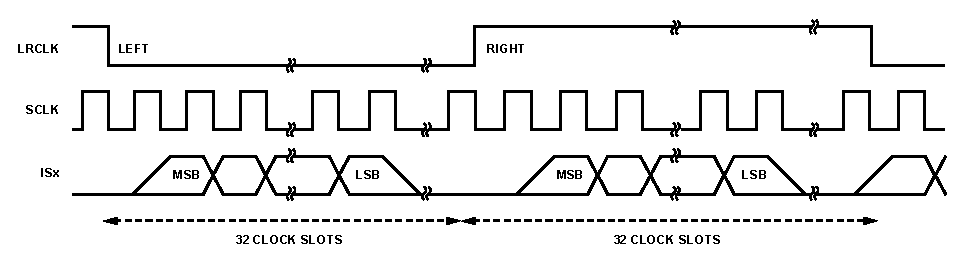
\includegraphics[width=1.0\textwidth]{audio_i2s}
		\caption{Ilustração dos sinais de som transmitidos no formato $I^{2}$S, retirada de \cite{R016}}
		\label{fig:i2s_audio}
	\end{center}
\end{figure}

Na placa recetora HDMI, que envia os dados para a FPGA Virtex-7, é também enviado o sinal \textit{Master Clock} que corresponde a um sinal de relógio de referência do sinais de áudio da entrada e ainda dados de áudio em AP0. É mencionado em \cite{R016} que estes dois sinais são referentes ao som no formato SPDIF e como tal não serão abordados neste projeto uma vez que as placas apenas suportam o formato $I^{2}$S.

Para além de dados de som e imagem são transmitidos dois bits com informação relativa ao estado do vídeo transmitido. Estes dados indicam o tipo e formato de vídeo que está a ser transmitidos e devem de seguida ser recebidos na placa transmissora. A combinação dos dois bits definem o estado do vídeo e são detalhadas em \cite{R014}.

Esta configuração acaba por ser bastante útil e será utilizada em diversas arquiteturas desenvolvidas uma vez que possui duas grandes vantagens: é capaz de suportar som e ao mesmo tempo não limita o formato da imagem transmitida a RGB. Em contrapartida, apenas suporta um canal (ao contrário da anterior), mas tal não é um problema pois apenas se pretende obter a transmissão num único canal entre dispositivo de fonte e dispositivo final HDMI. 


\subsubsection{Suporte de dois canais de imagem melhorado} \label{subsubsec:HDMIconfigMelhorado}


Esta configuração é capaz de suportar a transmissão de imagens em dois canais, tal como a configuração apresentada em \ref{subsubsec:HDMIconfigdefault} no entanto com alguns melhoramentos. A principal diferença consiste na capacidade de transmitir não só imagens em formato RGB mas também em YCbCr num dos canais. A tabela \ref{table:HDMI1canal_melhorado} do anexo \ref{ap1:HDMI} foi adaptada de \cite{R013} e apresenta detalhadamente todos os sinais transmitidos entre as placas HDMI e ainda os nomes dos conectores FMC.

Esta configuração na placa recetora transmite no canal 0 (RX0)  imagens tanto no formato RGB como YCbCr de 10 bits por cor e os sinais de controlo respectivos. Relativamente ao canal 1 dessa mesma placa (RX1) apenas é possível transmitir imagens em formato RGB de 10 bits por cor e os seus respetivos controlos. Para além disso, para cada canal são transmitidos dois bits que identificam o estado do vídeo que é transmitido, tal como já acontecia na configuração descrita em \ref{subsubsec:HDMIconfig+audio}.

Quando à placa transmissora quando configurada desta forma é capaz de receber nos dois canais (TX0 e TX1) imagens no formato RGB ou YCbCr com 10 bits por cor. Apesar de na tabela \ref{table:HDMI1canal_melhorado} o canal 1 definir os seus bits apenas para o caso de RGB, este canal também suporta na placa transmissora o formato YCbCr (e por isso a atribuição dos bits para TX1 assemelham-se ao canal TX0). Tal não é suportado no canal 1 da placa HDMI recetora (RX1) e por esse motivo a tabela está assim apresentada. À semelhança da placa recetora, a placa transmissora recebe 2 bits relativos à informação do vídeo que está a ser transferido, tal como a tabela \ref{table:HDMI1canal_melhorado} sugere.

\subsection{Configuração dos interruptores}

Neste capitulo serão descritas as configurações dos interruptores presentes nas placas HDMI para cada configuração existente. Tal é necessário definir para que os recetores e transmissores presentes nas placas possam enviar e receber imagens nos formatos que o utilizador pretende. Existem 8 interruptores que podem ser definidos pelo utilizador. Os interruptores entre S1-1 e S1-4 têm como função selecionar o tipo de formato que sai do recetor ADV7612 ou ADV7511 embebido na placa. Relativamente aos outros interruptores, raramente são utilizados e quando são a sua função não é relevante para o projeto e por isso não será especificada.

\subsubsection{Configuração por \textit{default}} \label{subsubsec:HDMIconfigdefault_switches}

Quando as placas estão configuras de fábrica, relembra-se que as imagens transmitidas correspondem ao formato RGB de 30 bits (10 bits por cor). Como tal, a indicação que vem em \cite{R009} sobre as funções dos interruptores da placa HDMI recetora é muito pouca. Apenas é indicado que quando esta configuração está ativa os interruptores se devem encontrar tal como especifica a tabela \ref{table:HDMI_default_switches_RX} na página \pageref{table:HDMI_default_switches_RX}.

\begin{table}[h!]
	\centering
	\begin{tabular}{|c|c|}
		\hline
		\textbf{Interruptor} & \textbf{Estado} \\ \hline
		\textbf{S1-1}        & ON              \\ \hline
		\textbf{S1-2}        & ON              \\ \hline
		\textbf{S1-3}        & ON              \\ \hline
		\textbf{S1-4}        & ON              \\ \hline
		\textbf{S1-5}        & Não usado       \\ \hline
		\textbf{S1-6}        & Não usado       \\ \hline
		\textbf{S1-7}        & Não usado       \\ \hline
		\textbf{S1-8}        & ON              \\ \hline
	\end{tabular}
	\caption{Configuração dos interruptores da placa HDMI RX configurada de fábrica, adaptada de \cite{R009}}
	\label{table:HDMI_default_switches_RX}
\end{table}

Relativamente à placa HDMI transmissora, é sabido que lhe chegam imagens no formato RGB de 10 bits, no entanto é possivel configurar o ADV7511 de tal forma que na sua saída o número de bits não seja limitado a 10. Para tal é necessário configurar os interruptores da forma que a tabela \ref{table:HDMI_default_switches_TX} indica.

 \begin{table}[h!]
	\centering
	\begin{tabular}{|c|c|c|c|}
		\hline
		\textbf{Interruptor} & \multicolumn{3}{c|}{\textbf{Estado}} \\ \hline
		\textbf{S1-1}        & OFF        & ON         & ON         \\ \hline
		\textbf{S1-2}        & ON         & ON         & OFF        \\ \hline
		\textbf{S1-3}        & ON         & OFF        & ON        \\ \hline
		\textbf{S1-4}        & ON         & ON         & ON         \\ \hline
		\textbf{OUTPUT}      & 8 bits     & 10 bits    & 12 bits    \\ \hline
		\textbf{S1-5}        & \multicolumn{3}{c|}{OFF}             \\ \hline
		\textbf{S1-6}        & \multicolumn{3}{c|}{Não usado}       \\ \hline
		\textbf{S1-7}        & \multicolumn{3}{c|}{Não usado}       \\ \hline
		\textbf{S1-8}        & \multicolumn{3}{c|}{Não usado}       \\ \hline
	\end{tabular}
	\caption{Configuração dos interruptores da placa HDMI RX configurada de fábrica, adaptada de \cite{R009}}
	\label{table:HDMI_default_switches_TX}
\end{table}
\subsubsection{Suporte de um canal de imagem e áudio} \label {subsubsec:HDMIconfig+audio_switches}

Quando se configuram as placas HDMI de forma a obter-se o suporte de áudio, então o formato da imagem transmitida também não é limitado a RGB. Desta maneira, o tabela \ref{table:HDMI_1ch+audio_switches_RX} indica como se devem configurar os interruptores de forma a obter-se na saída do ADV7612 as diversas possibilidades relativamente ao formato da imagem.
\begin{table}[h!]
	\centering
	\begin{tabular}{|c|c|c|c|c|c|c|}
		\hline
		\textbf{Interruptor}             & \multicolumn{6}{c|}{\textbf{Estado}}                                                                                                                                                                           \\ \hline
		\textbf{S1-1}                    & ON                                                        & OFF                                                       & ON                                                        & ON     & OFF     & ON      \\ \hline
		\textbf{S1-2}                    & ON                                                        & ON                                                        & OFF                                                       & ON     & ON      & OFF     \\ \hline
		\textbf{S1-3}                    & ON                                                        & ON                                                        & ON                                                        & OFF    & OFF     & OFF     \\ \hline
		\textbf{S1-4}                    & ON                                                        & ON                                                        & ON                                                        & ON     & ON      & ON      \\ \hline
		\multirow{2}{*}{\textbf{OUTPUT}} & \begin{tabular}[c]{@{}c@{}}YCbCr\\   444/422\end{tabular} & \begin{tabular}[c]{@{}c@{}}YCbCr\\   444/422\end{tabular} & \begin{tabular}[c]{@{}c@{}}YCbCr\\   444/422\end{tabular} & RGB    & RGB     & RGB     \\ \cline{2-7} 
		& 8 bits                                                    & 10 bits                                                   & 12 bits                                                   & 8 bits & 10 bits & 12 bits \\ \hline
		\textbf{S1-5}                    & \multicolumn{6}{c|}{ON}                                                                                                                                                                                        \\ \hline
		\textbf{S1-6}                    & \multicolumn{6}{c|}{ON}                                                                                                                                                                                        \\ \hline
		\textbf{S1-7}                    & \multicolumn{6}{c|}{ON}                                                                                                                                                                                        \\ \hline
		\textbf{S1-8}                    & \multicolumn{6}{c|}{ON}                                                                                                                                                                                        \\ \hline
	\end{tabular}
	\caption{Configuração dos interruptores da placa HDMI RX configurada para um canal e suporte de áudio, adaptada de \cite{R014}}
	\label{table:HDMI_1ch+audio_switches_RX}
\end{table}

À semelhança da placa recetora para esta configuração, também é possivel configurar o ADV7511 para se obter na sua saída diversos formatos de imagem. A tabela \ref{table:HDMI_1ch+audio_switches_TX} apresentada na página \pageref{table:HDMI_1ch+audio_switches_TX} indica essas mesmas combinações. 
\begin{table}[h!]
	\centering
	\begin{tabular}{|c|c|c|c|c|c|c|c|c|c|}
		\hline
		\textbf{Interruptor}             & \multicolumn{9}{c|}{\textbf{Estado}}                                                                                                                                                                                                                                                                                                                                       \\ \hline
		\textbf{S1-1}                    & ON                                                    & OFF                                                   & ON                                                    & ON                                                    & OFF                                                   & ON                                                    & ON     & OFF     & ON      \\ \hline
		\textbf{S1-2}                    & ON                                                    & ON                                                    & OFF                                                   & ON                                                    & ON                                                    & OFF                                                   & ON     & ON      & OFF     \\ \hline
		\textbf{S1-3}                    & ON                                                    & ON                                                    & ON                                                    & OFF                                                   & OFF                                                   & OFF                                                   & ON     & ON      & ON      \\ \hline
		\textbf{S1-4}                    & ON                                                    & ON                                                    & ON                                                    & ON                                                    & ON                                                    & ON                                                    & OFF    & OFF     & OFF     \\ \hline
		\multirow{2}{*}{\textbf{OUTPUT}} & \begin{tabular}[c]{@{}c@{}}YCbCr\\   444\end{tabular} & \begin{tabular}[c]{@{}c@{}}YCbCr\\   444\end{tabular} & \begin{tabular}[c]{@{}c@{}}YCbCr\\   444\end{tabular} & \begin{tabular}[c]{@{}c@{}}YCbCr\\   422\end{tabular} & \begin{tabular}[c]{@{}c@{}}YCbCr\\   422\end{tabular} & \begin{tabular}[c]{@{}c@{}}YCbCr\\   422\end{tabular} & RGB    & RGB     & RGB     \\ \cline{2-10} 
		& 8 bits                                                & 10 bits                                               & 12 bits                                               & 8 bits                                                & 10 bits                                               & 12 bits                                               & 8 bits & 10 bits & 12 bits \\ \hline
		\textbf{S1-5}                    & \multicolumn{9}{c|}{OFF}                                                                                                                                                                                                                                                                                                                                                   \\ \hline
		\textbf{S1-6}                    & \multicolumn{9}{c|}{Não usado}                                                                                                                                                                                                                                                                                                                                             \\ \hline
		\textbf{S1-7}                    & \multicolumn{9}{c|}{Não usado}                                                                                                                                                                                                                                                                                                                                             \\ \hline
		\textbf{S1-8}                    & \multicolumn{9}{c|}{ON}                                                                                                                                                                                                                                                                                                                                                    \\ \hline
	\end{tabular}
	\caption{Configuração dos interruptores da placa HDMI TX configurada para um canal e suporte de áudio, adaptada de \cite{R014}}
	\label{table:HDMI_1ch+audio_switches_TX}
\end{table}

\subsubsection{Suporte de dois canais de imagem melhorado} \label{subsubsec:HDMIconfigMelhorado_switches}

Quando se reconfigura as placas para suportarem a versão de transmissão de dois canais melhorada, é necessário ter em conta que existe um canal (canal 0) que tem a possibilidade de transmitir imagens tanto no formato YCbCr como RGB, porém o canal 1 apenas o faz no formato RGB. Na tabela \ref{table:HDMI_2ch_melhoradp_RX} da página \pageref{table:HDMI_2ch_melhoradp_RX} são apresentadas as configurações dos interruptores que configuram o ADV7612 de forma a enviar diferentes formatos.

\begin{table}[h!]
	\centering

	\begin{tabular}{|c|c|c|c|c|}
		\hline
		\textbf{Interruptor}             & \multicolumn{4}{c|}{\textbf{Estado}}             \\ \hline
		\textbf{S1-1}                    & ON            & OFF           & ON     & OFF     \\ \hline
		\textbf{S1-2}                    & ON            & ON            & ON     & ON      \\ \hline
		\textbf{S1-3}                    & ON            & ON            & OFF    & OFF     \\ \hline
		\textbf{S1-4}                    & ON            & ON            & ON     & ON      \\ \hline
		\multirow{2}{*}{\textbf{OUTPUT}} & YCbCr 444/422 & YCbCr 444/422 & RGB    & RGB     \\ \cline{2-5} 
		& 8 bits        & 10 bits       & 8 bits & 10 bits \\ \hline
		\textbf{S1-5}                    & \multicolumn{4}{c|}{ON}                          \\ \hline
		\textbf{S1-6}                    & \multicolumn{4}{c|}{ON}                          \\ \hline
		\textbf{S1-7}                    & \multicolumn{4}{c|}{ON}                          \\ \hline
		\textbf{S1-8}                    & \multicolumn{4}{c|}{ON}                          \\ \hline
	\end{tabular}
	\caption{Configuração dos interruptores da placa HDMI RX configurada para dois canais melhorados, adaptada de \cite{R013}}
	\label{table:HDMI_2ch_melhoradp_RX}
\end{table}

Relativamente à placa HDMI transmissora, ambos os canais são capazes de suportar imagens em formato RGB ou YCbCr. A tabela \ref{table:HDMI_2ch_melhoradp_TX} da página \pageref{table:HDMI_2ch_melhoradp_TX} apresenta as combinações dos interruptores para se poder obter os diversos formatos na saída do ADV7511.
\begin{table}[h!]
	\centering
	\begin{tabular}{|c|c|c|c|c|c|c|}
		\hline
		\textbf{Interruptor}             & \multicolumn{6}{c|}{\textbf{Estado}}                             \\ \hline
		\textbf{S1-1}                    & ON        & OFF       & ON        & OFF       & ON     & OFF     \\ \hline
		\textbf{S1-2}                    & ON        & ON        & ON        & ON        & ON     & ON      \\ \hline
		\textbf{S1-3}                    & ON        & ON        & OFF       & OFF       & ON     & ON      \\ \hline
		\textbf{S1-4}                    & ON        & ON        & ON        & ON        & OFF    & OFF     \\ \hline
		\multirow{2}{*}{\textbf{OUTPUT}} & YCbCr 444 & YCbCr 444 & YCbCr 422 & YCbCr 422 & RGB    & RGB     \\ \cline{2-7} 
		& 8 bits    & 10 bits   & 8 bits    & 10 bits   & 8 bits & 10 bits \\ \hline
		\textbf{S1-5}                    & \multicolumn{6}{c|}{OFF}                                         \\ \hline
		\textbf{S1-6}                    & \multicolumn{6}{c|}{Não usado}                                   \\ \hline
		\textbf{S1-7}                    & \multicolumn{6}{c|}{Não usado}                                   \\ \hline
		\textbf{S1-8}                    & \multicolumn{6}{c|}{ON}                                          \\ \hline
	\end{tabular}
	\caption{Configuração dos interruptores da placa HDMI RX configurada para dois canais melhorados, adaptada de \cite{R013}}
	\label{table:HDMI_2ch_melhoradp_TX} 
\end{table}
\section{Arquiteturas Desenvolvidas} \label{sec:HDMIarquiteturas}

Nesta secção passam a ser descritas as arquiteturas desenvolvidas e implementadas na FPGA referentes à comunicação entre as placas HDMI.  Por outras palavras, é feita uma aplicação daquilo que foi explicado sobre as placas HDMI a serem utilizadas até agora em arquiteturas implementadas e testadas em FPGA.

\subsection{Transmissão de uma imagem gerada na FPGA} \label{subsub:planA}

Numa fase inicil do projeto, optou-se por simplificar a transmissão e para tal utilizou-se apenas a placa transmissora HDMI configurada por defeito. Contrui-se em Verilog um bloco capaz de gerar uma imagem para ser transmitida, mais especificamente uma barra de cores, e utlizou-se essa imagem para ser transmitida pelos conectores FMC.

O bloco gerador de uma barra de cores foi adaptado de um bloco disponibilizado pela \textit{Inrenvium} aquando a compra das placas. Apesar de ter sido ligeiramente adaptado para este caso em especifico, este baseia-se essencialmente numa maquina de estados que vai contando as linhas e as colunas para que possa enviar não só os valores das cores de cada pixel, mas também os sinais de controlo como a sincronização vertical, a sincronização horizontal e ainda os valor de pixeis ativos.

Para que se entenda mais facilmente como e quando se transmitem os sinais de controlo da imagem e também os valor dos pixeis é demonstrado na imagem \ref{fig:colorBar_exemple} na página \pageref{fig:colorBar_exemple} uma exemplo de transmissão de uma imagem gerada na FPGA. Antes de passar para descrição da geração da imagem passam a ser descritos os acrónimos apresentados na figura:

\begin{enumerate}
	\item \textbf{HRES:} \textit{Horizontal Resolution} é o parâmetro que define a resolução horizontal da imagem que vai ser gerada pelo bloco, ou seja o número de pixeis em cada linha de transmissão.
	\item \textbf{HSW:} \textit{Horizontal Sync Width} é o parâmetro que define o número de ciclos de relógio que o sinal de sincronização horizontal tem.
	\item \textbf{HBP:} \textit{Horizontal Back Porch} é o parâmetro que define o número de pixeis que não contêm informação útil (relativamente à cor dos mesmos) antes de começar a ser transmitida a linha de imagem.
	\item \textbf{HFP:} \textit{Horizontal Front Porch} é o parâmetro que define o número de pixeis que não contem informação útil depois de ser transmitida uma linha da imagem.
	\item \textbf{VRES:} \textit{Vertical Resolution} é o parâmetro que define a resolução vertical da imagem que vai ser gerada pelo bloco, por outras palavras é o número de linhas de pixeis a ser geradas.
	\item \textbf{VSW:} \textit{Vertical Sync Width} é o parâmetro que define o número de linhas horizontais que o sinal de sincronização vertical está ativo.
	\item \textbf{VBP:} \textit{Vertical Back Porch} é o parâmetro que define o número de linhas horizontais que não contém informação útil relativamente ao pixeis antes de começarem a ser transmitidas as linhas de pixeis.
	\item \textbf{VFP:} \textit{Vertical Front Porch} é o parâmetro que define o número de linhas horizontais que não contém informação útil relativamente ao pixeis depois de terem sido transmitidas todas as linhas horizontais da imagem.
\end{enumerate}
	
\begin{figure}[h!]
	\begin{center}
		\leavevmode
		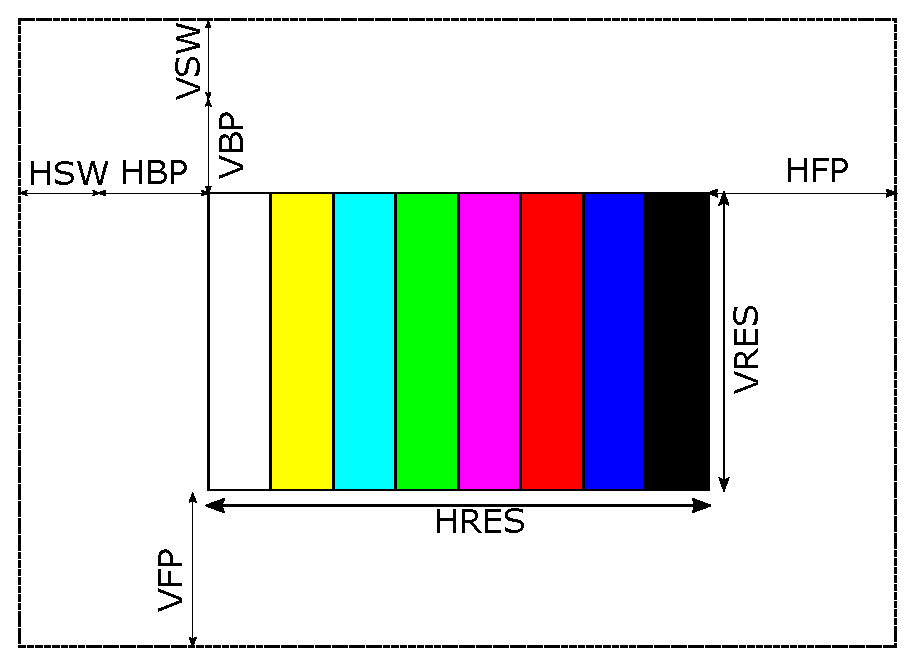
\includegraphics[width=1.0\textwidth]{exemplo_colorBar}
		\caption{Exemplo de imagem gerada pelo modulo desenvolvido}
		\label{fig:colorBar_exemple}
	\end{center}
\end{figure}

Para gerar uma imagem em \textit{FULL HD} cuja resolução é 1920x1080 pixeis e o sinal de relógio deve ter uma frequência de 148.5 MHz, foram o utilizados os seguintes valores para os parâmetro previamente descritos: HRES = 1920, HSW = 44, HBP = 44, HFP = 148,  VRES = 1080, VSW = 5, VBP = 36 e VFP = 4.

A figura \ref{fig:colorBar_fsm} na página \pageref{fig:colorBar_fsm} ilustra a maquina de estados desenvolvida para implementar a geração de uma barra a cores na FPGA. 

\begin{figure}[h!]
	\begin{center}
		\leavevmode
		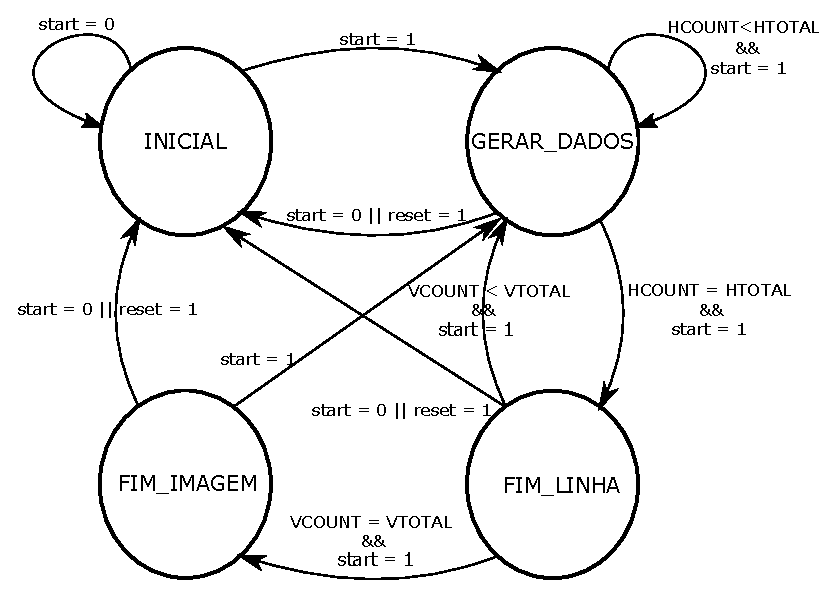
\includegraphics[width=1.0\textwidth]{colorBar_FSM}
		\caption{Máquina de estados para gerar uma barra de cores}
		\label{fig:colorBar_fsm}
	\end{center}
\end{figure}

Os registos VCOUNT E HCOUNT de decisão que se visualiza na figura correspondem a contadores que vão contanto pixel a pixel até ao fim de uma linha (no caso do HCOUNT) ou então de uma imagem inteira (no caso do VCOUNT). Os valores de HTOTAL e VTOTAL não são mais do que a soma de todo o tamanho dos dados na horizontal e na vertical respectivamente. Assim sendo, para este caso em especifico obtem-se os seguintes valores:
\begin{itemize}
	\item HTOTAL = HSW + HBP + HRES + HFP = 44 + 44 + 1920 + 148 = 2156
	\item VTOTAL = VSW + VBP + VRES + VFP = 5 + 36 + 1080 + 4 = 1125
\end{itemize}

Para além destes sinais de decisão para mudança de estado existem mais dois sinais no diagrama da máquina de estados presente na figura \ref{fig:colorBar_fsm} que ainda não foram mencionados que são o \textit{reset} e o \textit{start}. Estes dois sinais são botões do utilizador que lhe permitem definir quando se pretende que a transmissão esteja ativa ou desativa (através do botão \textit{start}) ou então quando se pretende restabelecer os dados originais da máquina de estados (através do botão \textit{reset}). 


Existem 4 estados nesta máquina eu consistem essencialmente em detecção do final de uma linha, e detecção do final de uma imagem e geração de dados. Os estados passam a ser descritos de seguida:

\begin{enumerate}
	\item \textbf{Estado inicial:} Neste estado são configurados os parâmetros para o inicio de uma transmissão, ou seja, os valores de HCOUNT e VCOUNT são igualados ao valor total do tamanho na horizontal e na vertical respectivamente. Por outras palavras, os valores de HCOUNT e VCOUNT são igualados a HTOTAL e VTOTAL respectivamente. Isto acontece porque é possivel retornar a este estado estando em qualquer um dos outros desde que seja pressionado o botão  de \textit{reset} ou então que a transmissão seja desligada pelo utilizador (\textit{start} = 0).
	\item \textbf{Estado para gerar dados:} Neste estado, ao flanco positivo do sinal de relógio do sistema, é incrementado o valor de HCOUNT e ao mesmo tempo são gerados os dados a serem transmitidos em cada ciclo de sinal de relógio, consoante o valor de HCOUNT e VCOUT. Quando o valor de HCOUNT se igualar ao valor de HTOTAL, então significa que foi transmitida uma linha inteira da imagem, e por isso a máquina transita de estado e o valor de VCOUNT volta a ser igualado a 1. O processo de geração de dados será explicado em XXXX
	\item \textbf{Estado de fim de linha:} Quando este estado está ativo, então uma linha da imagem foi transmitida, o que implica que é necessário incrementar o valor de linhas totais transmitidas (incrementando 1 valor em VCOUNT) e ainda verificar se a transmissão de uma imagem completa está realizada. Caso o valor de VCOUNT se iguale ao valor de VTOTAL, então transita-se para o estado de fim de imagem, e coloca-se o valor de VCOUNT a 1. Caso contrário, então a máquina transita para o estado que estava anteriormente.
	\item \textbf{Estado de fim de imagem} Quando este estado está ativo então significa que ambos os valores de HCOUNT e VCOUNT estão igualados a 1 e que por isso já foi transmitida uma imagem completa e como tal passa-se a transmitir uma próxima imagem, transitando novamente para o estado para gerar dados.
\end{enumerate}

Quando a máquina de estados se encontra no estado para gerar dados, então os dados de controlo são gerados nas seguintes condições :
\begin{itemize}
	\item \textbf{Sinal de sincronização vertical:} O sinal de sincronização vertical é um sinal que como já foi referido anteriormente indica o incio de transmissão de uma nova imagem, e por isso é ativado pela máquina de estados desenvolvida quando o valor em VCOUNT se igual ao valor de VTOTAL e quando o valor de HCOUNT se igual ao valor de HTOTAL, ou seja é ativado no final de uma imagem. Este sinal é ainda desligado quando o valor de VCOUNT se igual a VSW e o valor de HCOUNT se igual ao valor de HTOTAl, isto porque quando estas duas condições se verificam seignifica que o número de linhas em que o sinal de sincronização vertical deve estar ativo já terminou (é mesmo isso que o valor do parâmetro VSW define : \textit{Vertical Sync Width}).
	
	\item \textbf{Sinal de sincronização horizontal:} O sinal de sincronização horizontal indica o inicio de uma nova linha e como tal deve ser ativo sempre que o valor de HCOUNT se igual e ao valor de HTOTAL (porque indica o fim da emissão de uma linha). Da mesma maneira, este sinal deve ser desativo sempre que o valor de HCOUNT se igual ao valor de HSW, isto porque este valor indica que o período de tempo que este sinal deve estar ativo terminou.
	
	\item \textbf{Sinal de dados ativos:} Este sinal deve estar ativo sempre que se estiver a transmitir pixeis válidos, e por isso sempre que as condições que serão de seguida apresentadas se verificarem:
	\begin{enumerate}
		\item O valor de VCCOUNT é maior do que a soma entre VSW e VBP.
		\item O valor de VCOUNT é menor do que a soma entre VSW, VBP, VRES e 1.
		\item O valor de HCOUNT é maior do que a soma entre HSW, HBP subtraída de 1 valor.
		\item O valor de HCOUNT é menor do que a soma HSW, HBP e HRES.
	\end{enumerate}
	As duas primeira condições garantem que VCOUNT está na zona vertical que corresponde à transmissão de imagem na figura \ref{fig:colorBar_exemple}, e as duas ultimas condições garantem o mesmo mas na zona horizontal.
	\item \textbf{Valor dos pixeis:} Estes sinais correspondem a um barramento de 30 bits de uma imagem RGB com 10 bits por componente de cor. Como tal, estes valores devem corresponder a cores sempre o sinal de dados ativos estiver ligado e 0 sempre que estiver desligado. 
\end{itemize}

\begin{figure}[h!]
	\begin{center}
		\leavevmode
		\includegraphics[width=1.0\textwidth]{planA}
		\caption{Diagrama de blocos de arquitetura implementada utilizando um bloco gerador de barra de cores}
		\label{fig:planA}
	\end{center}
\end{figure}

Na figura \ref{fig:planA} é apresentado um diagrama de blocos da arquitetura implementada recorrendo a um bloco gerador de uma barra de cores. Este bloco foi implementado recorrendo-se à maquina de estados apresentada anteriormente.

Nas entradas do bloco estão ligados 4 sinais sendo que dois deles correspondem a um sinal de relógio diferencial de 200 MHz (\textit{clock\_p} corresponde ao sinal positivo e \textit{clock\_n} ao sinal negativo), e os outros dois sinais, \textit{start} e \textit{reset}, são sinais relevantes para a máquina de estados do bloco de geração de barras de cores definidos pelo utilizador e, por isso, são atribuídos a botões da FPGA. O sinal de relógio diferencial ligado às entradas deste bloco é proveniente do oscilador presente na FPGA e irá alimentar uma modulo que coloca na sua saída um sinal de relógio de 148.5 MHz. Esse módulo foi criado através do IP disponibilizado no VIVADO \textit{Clocking Wizard} que vem facilitar a geração de um sinal de relógio com a frequência pretendida tendo como uma base um sinal diferencial de 200 MHz. O sinal gerado, de 148.5 MHz, é o sinal de relógio principal do sistema uma vez que é a frequência necessária para gerar uma imagem em \textit{FULL HD}, e como tal é a essa cadência que os sinais serão enviados para a placa HDMI transmissora e é esse ainda o sinal de relógio da mesma.

Relativamente às saída do módulo é possivel visualizar na imagem \ref{fig:planA} que estas se encontram diretamente ligadas à placa transmissora HDMI através dos conectores FMC. Estes sinais são um barramento de 30 bits que corresponde ao pixel (\textit{pixel}), o sinal de sincronização horizontal (\textit{hsync}), o sinal de sincronização de vertical (\textit{vsync}) e ainda o sinal de dados ativos (\textit{enable}).

Para além do desenvolvimento do código em Verilog é necessário que as portas do modulo de topo, no caso desta arquitetura do modulo "planoA\_top.v", estejam atribuidas a portas físicas da FPGA. Para tal é necessário definir onde estão as localizações das portas na FPGA (LOC) e criar um ficheiro de defina essas mesmas restrições fisicas. A tabela \ref{table:LOCplanA_simples} na página \pageref{table:LOCplanA_simples} indica quais as localizações fisicas de cada porta existente no modulo de topo. No caso das portas que se conectam com a placa HDMI transmissora, estão representadas de forma abreviada, no entanto na tabela \ref{table:locPlanAdetail} do anexo \ref{ap3:LOCs} é possivel encontrar todas as portas com mais detalhes e ainda com informação sobre a ligação à placa HDMI transmissora.

\begin{longtable}[h!]
	{|c|c|c|c|}
	\hline
	\centering
%	\begin{tabular}
		\textbf{I/O} & \textbf{Sinal}        & \textbf{LOC na FPGA} & \textbf{Banco na FPGA} \\ \hline  \endhead
		I            & clk\_p                & E19                  & 38                     \\ \hline
		I            & clk\_n                & E18                  & 38                     \\ \hline
		I            & reset                 & N41                  & 19                     \\ \hline
		I            & start                 & E42                  & 19                     \\ \hline
		O            & cll\_px               & E34                  & 35                     \\ \hline
		O            & enable                & K35                  & 34                     \\ \hline
		O            & vsync                 & L31                  & 34                     \\ \hline
		O            & hsync                 & M32                  & 34                     \\ \hline
		O            & pixel{[}0{]}a{[}29{]} & (Ver anexo)          & 34 e 35                \\ \hline
%	\end{tabular}
	\caption{Localização das portas de entrada e saída da arquitetura}
	\label{table:LOCplanA_simples}
\end{longtable}

O ficheiro com estas restrições fisicas gerado após a atribuição das mesmas é apresentado no sub-capitulo \ref{ap2:planA_physical_cnstrs} do anexo \ref{ap2:codigo}. Para cada porta são atribuídas duas restrições: uma que indica a localização fisica na FPGA da porta e outra que indica a norma da mesma (\textit{IOSTANDARD}). A primeira permite atribuir a um determinado lugar físico da FPGA a porta que se pretende e a segunda define a norma dessa mesma porta para que todas as considerações que se tenham de ser tomadas relativamente a essa porta tenham em conta essa mesma norma.

Para além destas restrições fisicas geradas, são também geradas duas restrições temporais quanto aos sinais de relógio à entrada apresentadas no sub-capitulo \ref{ap2:planA_timing_cnstrs} do anexo \ref{ap2:codigo}. As retrições temporais existentes definem que nas portas de entrada do sinal de relógio diferencial existe um sinal com uma frequência de 200 MHz (periodo de 5ns). Isto porque este sinal de relógio é um sinal primário e como tal é importante que a ferramenta de implementação saiba o seu valor para poder garantir que toda a arquitetura cumpre os requisitos temporais.

Após a definição de todas as restrições e escrita do cófigo em verilg, a arquitetura desenvolvida foi devidamente implementada na FPGA e testada obtendo-se o previsto.

\subsection{Transmissão de imagem entre dispositivos HDMI} \label{subsub:planB}

Na arquitetura desenvolvida que é apresentada neste sub-capitulo são utilizadas as placas HDMI recetora e transmissora ambas configuradas por defeito e procede-se à transmissão de uma imagem entre dispositivos HDMI. O objetivo do desenvolvimento desta arquitetura consiste em obter uma ligação entre dois dispositivos ligados às placas HDMI de uma imagem RGB de 10 bits.

Foi desenvolvida uma arquitetura que recebe à cadência do sinal de relógio HDMI proveniente da placa (neste caso em especifico como é uma imagem \textit{FULL HD} é uma frequência de 148,5 MHz) os o resto dos sinais provenientes da mesma, mais especificamente o valor de \textit{pixel}, \textit{vsync}, \textit{hsync} e \textit{enable}. A imagem \ref{fig:planb1} da página \pageref{fig:planb1} ilustra o diagrama de blocos da arquitetura desenvolvida.

\begin{figure}[h!]
	\begin{center}
		\leavevmode
		\includegraphics[width=1.0\textwidth]{planB1}
		\caption{Diagram de blocos da arquitetura desenvolvida para transmitir imagem entre dispositivos HDMI}
		\label{fig:planb1}
	\end{center}
\end{figure}
%--> ENTRADA E SAIDA

É possivel visualizar que nesta arquitetura, tal como já acontecia na anterior, existem na sua saída os os sinais que são enviados para a placa HDMI transmisora e para além disso existem também os sinais provenientes da placa HDMI recetora. Também à semelhança da arquitetura descrita em \ref{subsub:planA} existem mais 4 sinais provenientes do exterior: o sinal de relógio diferencia de 200 MHz constituido pelo par positivo \textit{clock\_p} e pelo par negativo \textit{clock\_n}, e ainda o sinal \textit{start} que define o incio da transmissão da barra de cores em vez dos sinais provebientes da fonte HDMI e, por fim, o sinal de \textit{reset} que permite restabelecer os dados originais do sistema caso se pretenda.

%--> FUNCIONAMENTO DA MESMA
Os sinais que são recebidos à entrada são lidos para registos sincronos com o sinal de relógio proveniente da entrada (da placa HDMI recetora). Quando o sinal definido pelo utilizador \textit{start} está ativo os sinais seleccionados pelo multiplexador visivel na figura \ref{fig:planb1} são os sinais provenientes do modulo desenvolvido anteriormente que gera uma barra de cores. Esse mesmo sinal de start está ligado à entrada do bloco gerador da barra de cores para que quando ativo gere a imagem. Quando o sinal \textit{start} está desativo então obtém-se uma ligação entre as placas HDMI recetora e transmissora pois os sinais seleccionados pelo multiplexador são o sinais provenientes da entrada do modulo. Sempre que o sinal de \textit{reset} é ativo então todos os dados são repostos aos originais, como por exemplo os registos voltam ao estado original e também o bloco que produz a barra de cores.

A tabela \ref{table:LOCplanB_simples} na página \pageref{table:LOCplanB_simples} especifica as localizações fisicas da FPGA que foram atribuidas a cada porta do modulo desenvolvido e ainda o banco ao qual pertencem. As portas que fazem conexão com as placas HDMI transmissora e recetora são apresentadas nesta tabela de forma abreviada, no entanto na tabela \ref{table:LOCplanB_detail} do anexo \ref{ap3:LOCs} é possivel encontrar mais detalhamente as localizações dessas portas na FPGA bem como informação relativamente a esses sinais nas placas HDMI transmissora e recetora.

\begin{longtable}[h!]
	{|c|c|c|c|}
	\hline
	\centering
		\textbf{I/O} & \textbf{Sinal}              & \textbf{LOC na FPGA} & \textbf{Banco na FPGA} \\ \hline \endhead
		I            & clk\_p                      & E19                  & 38                     \\ \hline
		I            & clk\_n                      & E18                  & 38                     \\ \hline
		I            & reset                       & N41                  & 19                     \\ \hline
		I            & start                       & E42                  & 19                     \\ \hline
		I            & clk\_px\_in                 & AJ32                 & 14                     \\ \hline
		I            & enable\_in                  & AN38                 & 15                     \\ \hline
		I            & vsync\_in                   & AU38                 & 15                     \\ \hline
		I            & hsync\_in                   & AU39                 & 15                     \\ \hline
		I            & pixel\_in{[}0{]} a {[}29{]} & (Ver anexo)          & 14 e 15                \\ \hline
		O            & clock\_px                   & E34                  & 35                     \\ \hline
		O            & enable                      & K35                  & 34                     \\ \hline
		O            & vsync                       & L31                  & 34                     \\ \hline
		O            & hsync                       & M32                  & 34                     \\ \hline
		O            & pixel{[}0{]}a{[}29{]}       & (Ver anexo)            & 34 e 35                \\ \hline
		\caption{Localização das entradas e saídas das portas da arquitetura}
	\label{table:LOCplanB_simples}
\end{longtable}

%--> CONSTRAINTS %

A atribuição destas mesmas localizações das portas gerou um ficheiro de restrições físicas que é apresentado na secção \ref{ap2:planB_physical_cnstrs} do anexo \ref{ap2:codigo}. Relativamente a estas retrições físicas, existem para cada porta do modulo duas restrições: uma que define a localização fisica e outra a norma da fisica, tal como já foi mencionado anteriormente. 

Quanto às restrições temporais aplicadas ao sistema são idênticas às mesmas aplicadas na arquitetura desenvolvida anteriormente e estáo presentes em \ref{ap2:planB_timing_cnstrs} no anexo \ref{ap2:codigo}.
%--> RESULTADOS

Após sintese e implementação do código desenvolvido em verilog juntamente com as restrições aplicadas, a FPGA foi programada com esta arquitetura e foram obtidos os resultados esperados: obteve-se uma transmissão de imagem entre dois dispositivos HDMI. Foi utilizado um computador com saída HDMI como fonte de imagem conectado a placa HDMI RX, e desta maneira obteve-se no dispositivo HDMI de destino, que neste caso foi um monitor com entrada HDMI, conectado à placa HDMI transmissora a imagem transmitida.


\subsection{Transmissão de imagem e som entre dispositivos HDMI}

Após se obter uma ligação entre dois dispositivos HDMI de uma imagem, procedeu-se ao desenvolvimento de uma arquitetura capaz de trasmitir imagem e som. Para tal foi necessário reconfigurar as placas HDMI, tal como mencionado anteriormente, para a configuração que suporta apenas um canal mas que permite a transmissão de áudio em formato $I^{2}$S. As características desta configuração são apresentadas na secção \ref{subsubsec:HDMIconfig+audio} na página \pageref{subsubsec:HDMIconfig+audio} deste documento, mas é de notar que as imagens poderão ser transmitidas e recebidas em dois tipos de formatos (RGB ou YCbCr) e ainda com 8, 10 ou 12 bits por cor (dependendo da configuração dos interruptores das placas HDMI que estão especificados no sub-capitulo \ref{subsubsec:HDMIconfig+audio_switches}). Neste caso em especifico serão utilizados 12 bits por cor o que preferá um total de 36 bits por pixel.

Na imagem \ref{fig:planC} na página \pageref{fig:planC} é ilustrado um diagrama de blocos da arquitetura desenvolvida para se realizar a transmissão de imagem e som entre dois dispositivos HDMI. 

\begin{figure}[h!]
	\begin{center}
		\leavevmode
		\includegraphics[width=1.0\textwidth]{planC}
		\caption{Diagrama de blocos da arquitetura desenvolvida para transmitir imagem e som entre dispositivos HDMI}
		\label{fig:planC}
	\end{center}
\end{figure}

%--> ENTRADA E SAIDA
Através de uma breve observação do diagrama de blocos ilustrado é possivel concluir que existem mais portas tanto de entrada como de saída nesta arquitetura comparativamente às arquiteturas descritas previamente. Isto deve-se ao facto de agora haver a transmissão do som o que implica a transmissão de mais sinais. Assim sendo, na entrada encontram-se os sinais relativos às imagens à semelhança das arquiteturas anteriores: 36 bits de pixel, sinais de sincronização horizontal\textit{hsync} e vertical (\textit{vsync}) e ainda sinal que indica sinais de pixel ativos(\textit{enable}). Para além destes sinais provenientes da placa HDMI recetora, são recebidos os sinais referentes ao som: o sinal de relógio dos dados em série (\textit{sclk}), o sinal referente à seleccção do canal de audio esquerdo ou direto (\textit{lrclk}) e ainda os sinais que transportam os dados de som (de AP1 a AP4). Para além de dados de imagem e som há também um barramento de 2 bits que contém informação relativamente ao tipo de video que é transmitido (tal como já referido na secção \ref{subsubsec:HDMIconfig+audio}). Todos estes sinais que se encontram na entrada do modulo encontram-se também na saída pois é necessário enviar todos para a placa HDMI transmissora, no entanto o processo de transmissão dos mesmos passa a ser descrito.

Para além destes sinais provenientes e que são enviados para as palcas HDMI existem ainda mais portas do bloco. Existe o tipico sinal de relógio diferencia de 200 MHz definido na porta com \textit{clock\_p} pelo sinal positivo e como \textit{clock\_n} pelo sinal negativo. Este sinal de relógio proveniente do oscilador da FPGA serve como fonte para poder ser reproduzido o sinal de 148.5 MHz (frequência de uma imagem \textit{FULL HD}) que irá produzir a barra de cores no modulo "\textit{coloBar\_generator}". As outras três portas ainda não mencionadas são três sinais definidos pelo utilizador através de interruptores e botões. O sinal de \textit{reset} serve para repor todos os dados originais do sistema caso o utilizador pretenda. O sinal \textit{POWER} é o sinal que define a transmissão dos dados provenientes da placa HDMI recetora ou então da barra de cores, e o sinal \textit{MUTE} define a transmissão ou não dos sinais de som.

%% FUNCIONAMENTO DA MESMA

Os sinais de entrada relativos à imagem, tal como nas arquiteturas anteriores, são lidos para registos síncronos com o sinal de relógio de imagem (que no caso desta demonstração será 148.5 MHz pois são transmitidas imagens em \textit{FULL HD}). Estes mesmo sinais são enviados para a placa HDMI transmissora caso o sinal \textit{POWER} esteja ativo. Este sinal é um sinal que quando está desativo em vez de enviar para as saídas do modulo os sinais recebidos da placa HDMI recetora, envia os dados provenientes do bloco que reproduz uma barra de cores.

Relativamente aos dados referentes ao som, estes são também lidos para registos síncronos com o sinal de relógio referente à imagem proveniente da fonte HDMI pois numa fase mais avançada do projeto tal simplificação virá facilitar a transmissão dos dados em série a alta velocidade. Porém é necessário ter em consideração que estes dados variam a uma taxa que não é síncrona com o sinal de relógio da imagem, pois este possui uma frequência de 148,5 MHz para uma imagem no formato \textit{FULL HD}, e os dados de som variam a uma frequência de 3,072 MHz (tal como mencionado no sub-capitulo \ref{subsubsec:HDMIconfig+audio}). Assim sendo é necessário tomar as devidas precauções quando se faz o cruzamento entre estes dois domínios de relógio para que não sejam captados dados dos registos quando estes se encontram num estado de meta-estabilidade. Assim sendo, tal como sugerido em \cite{R024}, são utilizados dois registos síncronos com o sinal de relógio referente à imagem para que não haja propagações de erros.

O sinal de áudio enviado para as placas HDMI transmissora está dependente do valor do sinal de \textit{POWER} e \textit{MUTE}. Caso \textit{MUTE} esteja ativo o sinal de som não é transmitido e as entradas da placa HDMI são definidas com zero. O mesmo acontece quando o sinal de \textit{POWER} esteja desativo uma vez que indica que a transmissão da parte da placa HDMI recetora está desligada.

Mais uma vez é necessário definir as localizações fisicas de cada porta de entrada e saída do modulo principal, e como tal é possivel encontrar descritas essas mesmas atribuições na tabela \ref{table:LOCplanC_simples} na página \pageref{table:LOCplanC_simples}. Nessa mesma tabela os sinais que se conectam as placas HDMI são brevemente descritas, no entanto na tabela \ref{table:LOCplanC_detail} do anexo \ref{ap3:LOCs} essas mesmas conexões são descritas com mais detalhe.

\begin{longtable}[h!]
	{|c|c|c|c|}

		\hline
		\centering
\textbf{I/O} & \textbf{Sinal}               & \textbf{LOC na FPGA} & \textbf{Banco na FPGA} \\ \hline \endhead
I            & clk\_p                       & E19                  & 38                     \\ \hline
I            & clk\_n                       & E18                  & 38                     \\ \hline
I            & reset                        & N41                  & 19                     \\ \hline
I            & POWER                        & E42                  & 19                     \\ \hline
I            & MUTE                         & G41                  & 19                     \\ \hline
I            & clock\_p\_in                 & AJ32                 & 14                     \\ \hline
I            & vsync\_in                    & AU38                 & 15                     \\ \hline
I            & hsync\_in                    & AU39                 & 15                     \\ \hline
I            & enable\_in                   & AN38                 & 15                     \\ \hline
I            & pixel\_in{[}0{]} a {[}35{]}  & (Ver anexo)          & 14 e 15                \\ \hline
I            & sclk\_in                     & AJ37                 & 14                     \\ \hline
I            & lrclk\_in                    & AL35                 & 14                     \\ \hline
I            & AP1\_in                      & AL37                 & 14                     \\ \hline
I            & AP2\_in                      & AP35                 & 14                     \\ \hline
I            & AP3\_in                      & AM37                 & 14                     \\ \hline
I            & AP4\_in                      & AH33                 & 14                     \\ \hline
I            & info\_in{[}0{]}              & AV38                 & 15                     \\ \hline
I            & info\_in{[}1{]}              & AV39                 & 15                     \\ \hline
O            & clock\_p\_out                & E34                  & 35                     \\ \hline
O            & vsync\_out                   & L31                  & 34                     \\ \hline
O            & hsync\_out                   & M32                  & 34                     \\ \hline
O            & enable\_out                  & K35                  & 34                     \\ \hline
O            & pixel\_out{[}0{]} a {[}35{]} & (Ver anexo)          & 34 e 35                \\ \hline
O            & sclk\_out                    & A34                  & 35                     \\ \hline
O            & lrclk\_out                   & B33                  & 35                     \\ \hline
O            & AP1\_out                     & A36                  & 35                     \\ \hline
O            & AP2\_out                     & C39                  & 35                     \\ \hline
O            & AP3\_out                     & B38                  & 35                     \\ \hline
O            & AP4\_out                     & D32                  & 35                     \\ \hline
O            & info\_out{[}0{]}             & K32                  & 34                     \\ \hline
O            & info\_out{[}1{]}             & L32                  & 34                     \\ \hline   
	\caption{Localização das entradas e saídas das portas da arquitetura}
	\label{table:LOCplanC_simples}	
\end{longtable}

%--> CONSTRAINTS %

Para que a ferramenta de implementação reconheça as localizações fisicas da FPGA às quais são atribuídas as portas do bloco é gerado um ficheiro de restrições físicas semelhantes aos ficheiros gerados para as outras arquiteturas apresentadas até agora neste documento. O ficheiro que contém as restrições fisicas pode ser encontrado em \ref{ap2:planC_phisical_cnstrs} no anexo \ref{ap2:codigo}. Também à semelhança das arquiteturas anteriormente descritas foram geradas duas restrições temporais relativamente ao sinal de relógio diferencial à entrada que definem que na entrada existe um sinal com uma frequência de 200 MHz. Estas são apresentadas em \ref{ap2:planC_timing_cnstrs} no anexo \ref{ap2:codigo}.

%--> RESULTADOS

Esta arquitetura foi devidamente implementada na FPGA e testada, obtendo-se os resultados esperados. Apesar de os sinais de audio provenientes da placa HDMI recetora serem sincronos com sinal de relógio que não é o dos pixeis, o cruzamento estes dois dominios de relógio diferentes não apresentou qualquer tipo de problemas uma vez que ao ouvido humano os pequenos atrasados que possam eventualemente acontecer não são percetiveis. 
\chapter{Transmissão dos dados em série}\label{chap:Serie}


\chapter{Conclusões e Trabalho Futuro} \label{chap:concl}

Adicionar as siglas:

PROM - Programmable read-only memory


SPDIF

imp -> https://www.xilinx.com/support/answers/64340.html 
\chapter{Conclusões e Trabalho Futuro} \label{chap:concl}

\section{Qualidade dos resultados obtidos}

\section{Principais dificuldades encontradas}

-> Tempos de simulação comportamental, pos sintese, pos implementação elevados.

-> Tempos de sintese e implementação elevados

-> Informação pouco clara sobre o GTX

\section{Conclusões do projeto desenvolvido}

\section{Trabalho futuro}

-> Tornar a parte de serialização mais robusta 




%%----------------------------------------
%% Final materials
%%----------------------------------------

%% Bibliography
%% Comment the next command if BibTeX file not used, 
%% Assumes that bibliography is in ``myrefs.bib''
%%\PrintBib{myrefs}
\bibliographystyle{ieeetr}
\bibliography{myrefs}


%% Comment next 2 commands if numbered appendices are not used
\appendix
\chapter{Descrição das portas das placas HDMI} \label{ap1:HDMI}

Este anexo aborda detalhadamente as conexões que as placas HDMI têm disponíveis para conexão com a FPGA consoante a configuração das mesmas. São apresentados todos os pinos que transmitem dados, qual o nome da ligação desses pinos nas placas HDMI e ainda a descrição dos sinais.
\section{Configuração por omissão} \label{ap1:default}

Esta secção apresenta todas as portas das placas HDMI configuradas por omissão (tanto recetora como transmissora) que transmitem dados que são utilizados no projeto na tabela \ref{table:HDMIdataDefaultdetail}. De mencionar que esta configuração suporta dois canais (0 e 1), no entanto apenas são apresentadas as portas relativas ao canal 0 pois é o único utilizado no projeto.



\section{Suporte de um canal de imagem e áudio} \label {ap1:HDMIconfig+audio}

Nesta secção são apresentadas todas as portas das placas HDMI configuradas para terem suporte de imagem e áudio num canal que enviam dados para a FPGA utilizados no projeto. São apresentados os nomes das portas nas placas, os nomes dos sinais tanto do lado do recetor como do transmissor e a sua descrição. Tal informação é apresentada na tabela \ref{table:HDMI1canal+audioDETAIL}.

%\begin{longtable}[h!]
%	{@{}llll@{}}
%	\caption{Localização dos pinos de dados utilizados nas placas HDMI com a configuração de um canal e suporte de audio, adaptada de \cite{R014}}
%	\label{table:HDMI1canal+audioDETAIL}
%	\hline
%	\centering
%		\multicolumn{1}{c}{\textbf{PORTA}} & \multicolumn{1}{c}{\textbf{FPGA -\textgreater FMC (RX)}} & \multicolumn{1}{c}{\textbf{FMC -\textgreater FPGA (TX)}} & \multicolumn{1}{c}{\textbf{Descrição}} \\ \hline \endhead		
%		CLK0\_M2C\_P & RX\#0\_LLC                         & TX\#0\_DCLK                          & Sinal de relógio dos pixeis          \\ 
%		LA00\_P\_CC  & RX\#0\_VSYNC                       & TX\#0\_VSYNC                         & Sincronização vertical               \\ 
%		LA01\_P\_CC  & RX\#0\_HSYNC                       & TX\#0\_HSYNC                         & Sincronização horizontal             \\ 
%		LA02\_P      & RX\#0\_DE                          & TX\#0\_DE                            & Sinal de dados ativos                \\ 
%		LA03\_P      & RX\#0\_P0                          & TX\#0\_D0                            & Pixel de Imagem Cb{[}0{]}/B{[}0{]}   \\ 
%		LA04\_P      & RX\#0\_P1                          & TX\#0\_D1                            & Pixel de Imagem Cb{[}1{]}/B{[}1{]}   \\ 
%		LA05\_P      & RX\#0\_P2                          & TX\#0\_D2                            & Pixel de Imagem Cb{[}2{]}/B{[}2{]}   \\ 
%		LA06\_P      & RX\#0\_P3                          & TX\#0\_D3                            & Pixel de Imagem Cb{[}3{]}/B{[}3{]}   \\ 
%		LA07\_P      & RX\#0\_P4                          & TX\#0\_D4                            & Pixel de Imagem Cb{[}4{]}/B{[}4{]}   \\ 
%		LA08\_P      & RX\#0\_P5                          & TX\#0\_D5                            & Pixel de Imagem Cb{[}5{]}/B{[}5{]}   \\ 
%		LA09\_P      & RX\#0\_P6                          & TX\#0\_D6                            & Pixel de Imagem Cb{[}6{]}/B{[}6{]}   \\ 
%		LA10\_P      & RX\#0\_P7                          & TX\#0\_D7                            & Pixel de Imagem Cb{[}7{]}/B{[}7{]}   \\ 
%		LA11\_P      & RX\#0\_P8                          & TX\#0\_D8                            & Pixel de Imagem Cb{[}8{]}/B{[}8{]}   \\ 
%		LA12\_P      & RX\#0\_P9                          & TX\#0\_D9                            & Pixel de Imagem Cb{[}9{]}/B{[}9{]}   \\ 
%		LA13\_P      & RX\#0\_P10                         & TX\#0\_D10                           & Pixel de Imagem Cb{[}10{]}/B{[}10{]} \\ 
%		LA14\_P      & RX\#0\_P11                         & TX\#0\_D11                           & Pixel de Imagem Cb{[}11{]}/B{[}11{]} \\ 
%		LA15\_P      & RX\#0\_P12                         & TX\#0\_D12                           & Pixel de Imagem Y{[}0{]}/G{[}0{]}    \\ 
%		LA16\_P      & RX\#0\_P13                         & TX\#0\_D13                           & Pixel de Imagem Y{[}1{]}/G{[}1{]}    \\ 
%		LA17\_P\_CC  & RX\#0\_P14                         & TX\#0\_D14                           & Pixel de Imagem Y{[}2{]}/G{[}2{]}    \\ 
%		LA18\_P\_CC  & RX\#0\_P15                         & TX\#0\_D15                           & Pixel de Imagem Y{[}3{]}/G{[}3{]}    \\ 
%		LA19\_P      & RX\#0\_P16                         & TX\#0\_D16                           & Pixel de Imagem Y{[}4{]}/G{[}4{]}    \\ 
%		LA20\_P      & RX\#0\_P17                         & TX\#0\_D17                           & Pixel de Imagem Y{[}5{]}/G{[}5{]}    \\ 
%		LA21\_P      & RX\#0\_P18                         & TX\#0\_D18                           & Pixel de Imagem Y{[}6{]}/G{[}6{]}    \\ 
%		LA22\_P      & RX\#0\_P19                         & TX\#0\_D19                           & Pixel de Imagem Y{[}7{]}/G{[}7{]}    \\ 
%		LA23\_P      & RX\#0\_P20                         & TX\#0\_D20                           & Pixel de Imagem Y{[}8{]}/G{[}8{]}    \\ 
%		LA24\_P      & RX\#0\_P21                         & TX\#0\_D21                           & Pixel de Imagem Y{[}9{]}/G{[}9{]}    \\ 
%		LA25\_P      & RX\#0\_P22                         & TX\#0\_D22                           & Pixel de Imagem Y{[}10{]}/G{[}10{]}  \\ 
%		LA26\_P      & RX\#0\_P23                         & TX\#0\_D23                           & Pixel de Imagem Y{[}11{]}/G{[}11{]}  \\ 
%		LA27\_P      & RX\#0\_P24                         & TX\#0\_D24                           & Pixel de Imagem Cr{[}0{]}/R{[}0{]}   \\ 
%		LA28\_P      & RX\#0\_P25                         & TX\#0\_D25                           & Pixel de Imagem Cr{[}1{]}/R{[}1{]}   \\ 
%		LA29\_P      & RX\#0\_P26                         & TX\#0\_D26                           & Pixel de Imagem Cr{[}2{]}/R{[}2{]}   \\ 
%		LA30\_P      & RX\#0\_P27                         & TX\#0\_D27                           & Pixel de Imagem Cr{[}3{]}/R{[}3{]}   \\ 
%		LA31\_P      & RX\#0\_P28                         & TX\#0\_D28                           & Pixel de Imagem Cr{[}4{]}/R{[}4{]}   \\ 
%		LA32\_P      & RX\#0\_P29                         & TX\#0\_D29                           & Pixel de Imagem Cr{[}5{]}/R{[}5{]}   \\ 
%		LA00\_N\_CC & \begin{tabular}[l]{@{}l@{}}RX\#0\_Input \\ video status{[}0{]}\end{tabular}   & \begin{tabular}[l]{@{}l@{}}TX\#0\_Input \\ video status{[}0{]}\end{tabular} & Formato do video (2D/3D) 			   \\ 
%	
%		LA01\_N\_CC & \begin{tabular}[l]{@{}l@{}}RX\#0\_Input \\ video status{[}1{]}\end{tabular}    & \begin{tabular}[l]{@{}l@{}}TX\#0\_Input \\ video status{[}1{]}\end{tabular}       & Formato do video (2D/3D)   \\ 
%		LA19\_N      & RX\#0\_MCLK                        & TX\#0\_MCLK                          & \textit{Master Clock} de som     \\ 
%		LA20\_N      & RX\#0\_SCLK                        & TX\#0\_SCLK                          & \textit{Serial Clock} de som     \\ 
%		LA21\_N      & RX\#0\_AP0                         & TX\#0\_AP0                           & Dados de Som SPDIF                   \\ 
%		LA22\_N      & RX\#0\_AP1                         & TX\#0\_AP1                           & Dados de Som I2S {[}0{]}             \\ 
%		LA23\_N      & RX\#0\_AP2                         & TX\#0\_AP2                           & Dados de Som I2S {[}1{]}             \\ 
%		LA24\_N      & RX\#0\_AP3                         & TX\#0\_AP3                           & Dados de Som I2S {[}2{]}             \\ 
%		LA25\_N      & RX\#0\_AP4                         & TX\#0\_AP4                           & Dados de Som I2S {[}3{]}             \\ 
%		LA26\_N      & RX\#0\_AP5                         & TX\#0\_AP5                           & Sinal de relógio LR (left/right)     \\ 
%		LA27\_N      & RX\#0\_P30                         & TX\#0\_D30                           & Pixel de Imagem Cr{[}6{]}/R{[}6{]}   \\ 
%		LA28\_N      & RX\#0\_P31                         & TX\#0\_D31                           & Pixel de Imagem Cr{[}7{]}/R{[}7{]}   \\ 
%		LA29\_N      & RX\#0\_P32                         & TX\#0\_D32                           & Pixel de Imagem Cr{[}8{]}/R{[}8{]}   \\ 
%		LA30\_N      & RX\#0\_P33                         & TX\#0\_D33                           & Pixel de Imagem Cr{[}9{]}/R{[}9{]}   \\ 
%		LA31\_N      & RX\#0\_P34                         & TX\#0\_D34                           & Pixel de Imagem Cr{[}10{]}/R{[}10{]} \\ 
%		LA32\_N      & RX\#0\_P35                         & TX\#0\_D35                           & Pixel de Imagem Cr{[}11{]}/R{[}11{]} \\ \hline
%\end{longtable}

\section{Suporte de dois canais de imagem melhorado} \label{ap1:HDMIconfigMelhorado}

Nesta secção são apresentados os dados enviados pelas placas HDMI configuradas para a versão de suporte de imagem em dois canais melhorada. Para cada porta são apresentados os nomes dos sinais tanto na placa transmissora como recetora e também é descrito o seu funcionamento. De notar que esta configuração suporta dois canais, mas na tabela \ref{table:HDMI1canal_melhorado} apenas é apresentado o canal 0, visto que o canal 1 não é utilizado.
\\

%
%\begin{longtable}[h!]
%	{@{}llll@{}}
%	\caption{Localização dos pinos de dados utilizados nas placas HDMI com a configuração de suporte de dois canais melhorado, adaptada de \cite{R013}}
%	\label{table:HDMI1canal_melhorado}
%	\hline
%	\centering
%	\multicolumn{1}{c}{\textbf{PORTA}} & \multicolumn{1}{c}{\textbf{FPGA -\textgreater FMC (RX)}} & \multicolumn{1}{c}{\textbf{FMC -\textgreater FPGA (TX)}} & \multicolumn{1}{c}{\textbf{Descrição}} \\ \hline \endhead
%	CLK0\_M2C\_P & RX\#0\_LLC          				& TX\#0\_DCLK                          & Sinal de relógio dos pixeis 			\\ 
%	%CLK1\_M2C\_N & RX\#1\_LLC           			 & TX\#1\_DCLK                          & Sinal de relógio dos pixeis 			\\ \hline
%	LA00\_P\_CC  & RX\#0\_VSYNC         			  & TX\#0\_VSYNC                         & Sincronização vertical         		\\ 
%	LA01\_P\_CC  & RX\#0\_HSYNC         		  & TX\#0\_HSYNC                         & Sincronização horizontal       		\\ 
%	LA02\_P      & RX\#0\_DE            				   & TX\#0\_DE                            & Sinal de dados ativos          		\\
%	LA03\_P      & RX\#0\_P0            				   & TX\#0\_D0                            & Pixel de Imagem Cb{[}0{]}/B{[}0{]}   \\
%	LA04\_P      & RX\#0\_P1            		      & TX\#0\_D1                            & Pixel de Imagem Cb{[}1{]}/B{[}1{]}   \\ 
%	LA05\_P      & RX\#0\_P2            			      & TX\#0\_D2                            & Pixel de Imagem Cb{[}2{]}/B{[}2{]}   \\ 
%	LA06\_P      & RX\#0\_P3            			      & TX\#0\_D3                            & Pixel de Imagem Cb{[}3{]}/B{[}3{]}   \\ 
%	LA07\_P      & RX\#0\_P4            			      & TX\#0\_D4                            & Pixel de Imagem Cb{[}4{]}/B{[}4{]}   \\ 
%	LA08\_P      & RX\#0\_P5            			      & TX\#0\_D5                            & Pixel de Imagem Cb{[}5{]}/B{[}5{]}   \\ 
%	LA09\_P      & RX\#0\_P6            		     & TX\#0\_D6                            & Pixel de Imagem Cb{[}6{]}/B{[}6{]}   \\ 
%	LA10\_P      & RX\#0\_P7            			     & TX\#0\_D7                            & Pixel de Imagem Cb{[}7{]}/B{[}7{]}   \\
%	LA11\_P      & RX\#0\_P8            			     & TX\#0\_D8                            & Pixel de Imagem Cb{[}8{]}/B{[}8{]}   \\ 
%	LA12\_P      & RX\#0\_P9            		      & TX\#0\_D9                            & Pixel de Imagem Cb{[}9{]}/B{[}9{]}   \\
%	LA13\_P      & RX\#0\_P10           		      & TX\#0\_D10                           &Pixel de Imagem Y{[}0{]}/G{[}0{]} 	\\ 
%	LA14\_P      & RX\#0\_P11           		     & TX\#0\_D11                           & Pixel de Imagem Y{[}1{]}/G{[}1{]}	\\ 
%	LA15\_P      & RX\#0\_P12          				     & TX\#0\_D12                           & Pixel de Imagem Y{[}2{]}/G{[}2{]}    \\
%	LA16\_P      & RX\#0\_P13           			      & TX\#0\_D13                           & Pixel de Imagem Y{[}3{]}/G{[}3{]}    \\ 
%	LA17\_P\_CC  & RX\#0\_P14           		  & TX\#0\_D14                           & Pixel de Imagem Y{[}4{]}/G{[}4{]}    \\ 
%	LA18\_P\_CC  & RX\#0\_P15           		  & TX\#0\_D15                           & Pixel de Imagem Y{[}5{]}/G{[}5{]}    \\ 
%	LA19\_P      & RX\#0\_P16           			      & TX\#0\_D16                           & Pixel de Imagem Y{[}6{]}/G{[}6{]}   	\\ 
%	LA20\_P      & RX\#0\_P17           			      & TX\#0\_D17                           & Pixel de Imagem Y{[}7{]}/G{[}7{]}    \\ 
%	LA21\_P      & RX\#0\_P18           		      & TX\#0\_D18                           & Pixel de Imagem Y{[}8{]}/G{[}8{]}    \\ 
%	LA22\_P      & RX\#0\_P19           			     & TX\#0\_D19                           & Pixel de Imagem Y{[}9{]}/G{[}9{]}    \\
%	LA23\_P      & RX\#0\_P20           		      & TX\#0\_D20                           & Pixel de Imagem Cr{[}0{]}/R{[}0{]}    \\ 
%	LA24\_P      & RX\#0\_P21           		     & TX\#0\_D21                           & Pixel de Imagem Cr{[}1{]}/R{[}1{]}   \\ 
%	LA25\_P      & RX\#0\_P22           		      & TX\#0\_D22                           & Pixel de Imagem Cr{[}2{]}/R{[}2{]}  \\ 
%	LA26\_P      & RX\#0\_P23          			     & TX\#0\_D23                           & Pixel de Imagem Cr{[}3{]}/R{[}3{]}  \\ 
%	LA27\_P      & RX\#0\_P24           			      & TX\#0\_D24                           & Pixel de Imagem Cr{[}4{]}/R{[}4{]}  \\ 
%	LA28\_P      & RX\#0\_P25           		      & TX\#0\_D25                           & Pixel de Imagem Cr{[}5{]}/R{[}5{]}   \\
%	LA29\_P      & RX\#0\_P26           		      & TX\#0\_D26                           & Pixel de Imagem Cr{[}6{]}/R{[}6{]}   \\ 
%	LA30\_P      & RX\#0\_P27           		      & TX\#0\_D27                           & Pixel de Imagem Cr{[}7{]}/R{[}7{]}   \\ 
%	LA31\_P      & RX\#0\_P28           			      & TX\#0\_D28                           & Pixel de Imagem Cr{[}8{]}/R{[}8{]}   \\
%	LA32\_P      & RX\#0\_P29           		      & TX\#0\_D29                           & Pixel de Imagem Cr{[}9{]}/R{[}9{]}   	\\ 
%	
%	CLK0\_M2C\_N & \begin{tabular}[l]{@{}l@{}}RX\#0\_Input \\ video status{[}0{]}\end{tabular}   & \begin{tabular}[l]{@{}l@{}}TX\#0\_Input \\ video status{[}0{]}\end{tabular} & Formato do video (2D/3D) 			   \\ 
%		
%	CLK1\_M2C\_N & \begin{tabular}[l]{@{}l@{}}RX\#0\_Input \\ video status{[}1{]}\end{tabular}    & \begin{tabular}[l]{@{}l@{}}TX\#0\_Input \\ video status{[}1{]}\end{tabular}       & Formato do video (2D/3D)   \\ 
%%	LA33\_P      & \begin{tabular}[c]{@{}c@{}}RX\#1\_Input \\ video status{[}0{]}\end{tabular}    	   & \begin{tabular}[c]{@{}c@{}}TX\#1\_Input \\ video status{[}0{]}\end{tabular}       & Formato do video (2D/3D) 			   \\ \hline
%%	LA33\_N      & \begin{tabular}[c]{@{}c@{}}RX\#1\_Input \\ video status{[}1{]}\end{tabular}   	   & \begin{tabular}[c]{@{}c@{}}TX\#1\_Input \\ video status{[}1{]}\end{tabular}       & Formato do video (2D/3D) 			   \\ \hline
%%	LA00\_N\_CC  & RX\#1\_VSYNC                      & TX\#1\_VSYNC                         & Sincronização vertical         		\\ \hline
%%	LA01\_N\_CC  & RX\#1\_HSYNC                     & TX\#1\_HSYNC                         & Sincronização horizontal       		\\ \hline
%%	LA02\_N      & RX\#1\_DE                        & TX\#1\_DE                            & Sinal de dados ativos          		\\ \hline
%%	LA03\_N      & RX\#1\_P0                         & TX\#1\_D0                            & Pixel de Imagem B{[}0{]}   \\ \hline
%%	LA04\_N      & RX\#1\_P1                        & TX\#1\_D1                            & Pixel de Imagem B{[}1{]}   \\ \hline
%%	LA05\_N      & RX\#1\_P2                         & TX\#1\_D2                            & Pixel de Imagem B{[}2{]}   \\ \hline
%%	LA06\_N      & RX\#1\_P3                         & TX\#1\_D3                            & Pixel de Imagem B{[}3{]}   \\ \hline
%%	LA07\_N      & RX\#1\_P4                        & TX\#1\_D4                            & Pixel de Imagem B{[}4{]}   \\ \hline
%%	LA08\_N      & RX\#1\_P5                       & TX\#1\_D5                            & Pixel de Imagem B{[}5{]}   \\ \hline
%%	LA09\_N      & RX\#1\_P6                         & TX\#1\_D6                            & Pixel de Imagem B{[}6{]}   \\ \hline
%%	LA10\_N      & RX\#1\_P7                        & TX\#1\_D7                            & Pixel de Imagem B{[}7{]}   \\ \hline
%%	LA11\_N      & RX\#1\_P8                        & TX\#1\_D8                            & Pixel de Imagem B{[}8{]}   \\ \hline
%%	LA12\_N      & RX\#1\_P9                        & TX\#1\_D9                            & Pixel de Imagem B{[}9{]}   \\ \hline
%%	LA13\_N      & RX\#1\_P10                        & TX\#1\_D10                           & Pixel de Imagem G{[}0{]} 	\\ \hline
%%	LA14\_N      & RX\#1\_P11                        & TX\#1\_D11                           & Pixel de Imagem G{[}1{]}	\\ \hline
%%	LA15\_N      & RX\#1\_P12                      & TX\#1\_D12                           & Pixel de Imagem G{[}2{]}    \\ \hline
%%	LA16\_N      & RX\#1\_P13                      & TX\#1\_D13                           & Pixel de Imagem G{[}3{]}    \\ \hline
%%	LA17\_N\_CC  & RX\#1\_P14                        & TX\#1\_D14                           & Pixel de Imagem G{[}4{]}    \\ \hline
%%	LA18\_N\_CC  & RX\#1\_P15                        & TX\#1\_D15                           & Pixel de Imagem G{[}5{]}    \\ \hline
%%	LA19\_N      & RX\#1\_P16                        & TX\#1\_D16                           & Pixel de Imagem G{[}6{]}   	\\ \hline
%%	LA20\_N      & RX\#1\_P17                        & TX\#1\_D17                           & Pixel de Imagem G{[}7{]}    \\ \hline
%%	LA21\_N      & RX\#1\_P18                       & TX\#1\_D18                           & Pixel de Imagem G{[}8{]}    \\ \hline
%%	LA22\_N      & RX\#1\_P19                       & TX\#1\_D19                           & Pixel de Imagem G{[}9{]}    \\ \hline
%%	LA23\_N      & RX\#1\_P20                       & TX\#1\_D20                           & Pixel de Imagem R{[}0{]}    \\ \hline
%%	LA24\_N      & RX\#1\_P21                       & TX\#1\_D21                           & Pixel de Imagem R{[}1{]}   \\ \hline
%%	LA25\_N      & RX\#1\_P22                       & TX\#1\_D22                           & Pixel de Imagem R{[}2{]}  \\ \hline
%%	LA26\_N      & RX\#1\_P23                      & TX\#1\_D23                           & Pixel de Imagem R{[}3{]}  \\ \hline
%%	LA27\_N      & RX\#1\_P24                        & TX\#1\_D24                           & Pixel de Imagem R{[}4{]}  \\ \hline
%%	LA28\_N      & RX\#1\_P25                      & TX\#1\_D25                           & Pixel de Imagem R{[}5{]}   \\ \hline
%%	LA29\_N      & RX\#1\_P26                      & TX\#1\_D26                           & Pixel de Imagem R{[}6{]}   \\ \hline
%%	LA30\_N      & RX\#1\_P27                       & TX\#1\_D27                           & Pixel de Imagem R{[}7{]}   \\ \hline
%%	LA31\_N      & RX\#1\_P28                       & TX\#1\_D28                           & Pixel de Imagem R{[}8{]}   \\ \hline
%%	LA32\_N      & RX\#1\_P29                       & TX\#1\_D29                           & Pixel de Imagem R{[}9{]}   	\\ \hline
%	\hline
%\end{longtable}
{\tiny \chapter{Configurações dos interruptores das placas HDMI} \label{ap4:switches}}

Este anexo contempla as diversas configurações possíveis dos interruptores presentes nas placas HDMI para as diferentes configurações das mesmas.

\section{Configuração por omissão} \label{sec:HDMIconfigdefault_switches}

Quando as placas estão configuradas de fábrica relembra-se que as imagens transmitidas correspondem ao formato RGB de 30 bits (10 bits por cor). Deste modo, a indicação que vem em \cite{R009} sobre as funções dos interruptores da placa HDMI recetora é muito pouca. Apenas é indicado que quando esta configuração está ativa os interruptores se devem encontrar tal como especifica a tabela \ref{table:HDMI_default_switches_RX} na página \pageref{table:HDMI_default_switches_RX}, adaptada de \cite{R009}.

%\begin{table}[h!]
%	\centering
%	\begin{tabular}{|c|c|}
%		\hline
%		\textbf{Interruptor} & \textbf{Estado} \\ \hline
%		\textbf{S1-1}        & ON              \\ \hline
%		\textbf{S1-2}        & ON              \\ \hline
%		\textbf{S1-3}        & ON              \\ \hline
%		\textbf{S1-4}        & ON              \\ \hline
%		\textbf{S1-5}        & Não usado       \\ \hline
%		\textbf{S1-6}        & Não usado       \\ \hline
%		\textbf{S1-7}        & Não usado       \\ \hline
%		\textbf{S1-8}        & ON              \\ \hline
%	\end{tabular}
%	\caption{Configuração dos interruptores da placa HDMI RX configurada de fábrica, adaptada de \cite{R009}}
%	\label{table:HDMI_default_switches_RX}
%\end{table}


\begin{table}[h!]
	\centering

		\begin{tabular}{@{}ll@{}}
			\toprule
			\multicolumn{1}{c}{\textbf{Interruptor}} & \multicolumn{1}{c}{\textbf{Estado}} \\ \midrule
			\textbf{S1-1}                            & ON                                  \\
			\textbf{S1-2}                            & ON                                  \\
			\textbf{S1-3}                            & ON                                  \\
			\textbf{S1-4}                            & ON                                  \\
			\textbf{S1-5}                            & Não usado                           \\
			\textbf{S1-6}                            & Não usado                           \\
			\textbf{S1-7}                            & Não usado                           \\
			\textbf{S1-8}                            & ON                                  \\ \bottomrule
		\end{tabular}%
	\captionsetup{width=0.3\linewidth}
	\caption{Configuração dos interruptores da placa HDMI RX configurada de fábrica}
	\label{table:HDMI_default_switches_RX}
\end{table}

Relativamente à placa HDMI transmissora é sabido que lhe chegam imagens no formato RGB de 10 bits. Todavia é possível configurar o integrado ADV7511 de tal forma que na sua saída o número de bits não seja limitado a 10. Para tal é necessário configurar os interruptores da forma que a tabela \ref{table:HDMI_default_switches_TX} indica, adaptada de \cite{R009}.

%\begin{table}[h!]
%	\centering
%	\begin{tabular}{|c|c|c|c|}
%		\hline
%		\textbf{Interruptor} & \multicolumn{3}{c|}{\textbf{Estado}} \\ \hline
%		\textbf{S1-1}        & OFF        & ON         & ON         \\ \hline
%		\textbf{S1-2}        & ON         & ON         & OFF        \\ \hline
%		\textbf{S1-3}        & ON         & OFF        & ON        \\ \hline
%		\textbf{S1-4}        & ON         & ON         & ON         \\ \hline
%		\textbf{OUTPUT}      & 8 bits     & 10 bits    & 12 bits    \\ \hline
%		\textbf{S1-5}        & \multicolumn{3}{c|}{OFF}             \\ \hline
%		\textbf{S1-6}        & \multicolumn{3}{c|}{Não usado}       \\ \hline
%		\textbf{S1-7}        & \multicolumn{3}{c|}{Não usado}       \\ \hline
%		\textbf{S1-8}        & \multicolumn{3}{c|}{Não usado}       \\ \hline
%	\end{tabular}
%	\caption{Configuração dos interruptores da placa HDMI RX configurada de fábrica, adaptada de \cite{R009}}
%	\label{table:HDMI_default_switches_TX}
%\end{table}

\begin{table}[h!]
	\centering
	\begin{tabular}{@{}llll@{}}
		\toprule
		\multicolumn{1}{c}{\textbf{Interruptor}} & \multicolumn{3}{c}{\textbf{Estado}} \\ \midrule
		\multicolumn{1}{l|}{\textbf{S1-1}} & OFF & ON & ON \\
		\multicolumn{1}{l|}{\textbf{S1-2}} & ON & ON & OFF \\
		\multicolumn{1}{l|}{\textbf{S1-3}} & ON & OFF & ON \\
		\multicolumn{1}{l|}{\textbf{S1-4}} & ON & ON & ON \\
		\multicolumn{1}{l|}{\textbf{\textit{Output}}} & 8 bits & 10 bits & 12 bits \\
		\multicolumn{1}{l|}{\textbf{S1-5}} & \multicolumn{3}{l}{Não usado} \\
		\multicolumn{1}{l|}{\textbf{S1-6}} & \multicolumn{3}{l}{Não usado} \\
		\multicolumn{1}{l|}{\textbf{S1-7}} & \multicolumn{3}{l}{Não usado} \\
		\multicolumn{1}{l|}{\textbf{S1-8}} & \multicolumn{3}{l}{Não usado} \\ \bottomrule
	\end{tabular}
	\captionsetup{width=0.45\linewidth}
	\caption{Configuração dos interruptores da placa HDMI TX configurada de fábrica}
	\label{table:HDMI_default_switches_TX}
\end{table}


\section{Suporte de um canal de imagem e áudio} \label {sec:HDMIconfig+audio_switches}

Quando se configuram as placas HDMI de forma a obter-se o suporte de imagem e som o formato da imagem transmitida também não é limitado ao RGB. Desta maneira, a tabela \ref{table:HDMI_1ch+audio_switches_RX} indica como se devem configurar os interruptores de forma a obter-se na saída do ADV7612 as diversas possibilidades relativamente ao formato da imagem e foi adaptada de \cite{R014}.

%\begin{table}[h!]
%	\centering
%	\begin{tabular}{|c|c|c|c|c|c|c|}
%		\hline
%		\textbf{Interruptor}             & \multicolumn{6}{c|}{\textbf{Estado}}                                                                                                                                                                           \\ \hline
%		\textbf{S1-1}                    & ON                                                        & OFF                                                       & ON                                                        & ON     & OFF     & ON      \\ \hline
%		\textbf{S1-2}                    & ON                                                        & ON                                                        & OFF                                                       & ON     & ON      & OFF     \\ \hline
%		\textbf{S1-3}                    & ON                                                        & ON                                                        & ON                                                        & OFF    & OFF     & OFF     \\ \hline
%		\textbf{S1-4}                    & ON                                                        & ON                                                        & ON                                                        & ON     & ON      & ON      \\ \hline
%		\multirow{2}{*}{\textbf{OUTPUT}} & \begin{tabular}[c]{@{}c@{}}YCbCr\\   444/422\end{tabular} & \begin{tabular}[c]{@{}c@{}}YCbCr\\   444/422\end{tabular} & \begin{tabular}[c]{@{}c@{}}YCbCr\\   444/422\end{tabular} & RGB    & RGB     & RGB     \\ \cline{2-7} 
%		& 8 bits                                                    & 10 bits                                                   & 12 bits                                                   & 8 bits & 10 bits & 12 bits \\ \hline
%		\textbf{S1-5}                    & \multicolumn{6}{c|}{ON}                                                                                                                                                                                        \\ \hline
%		\textbf{S1-6}                    & \multicolumn{6}{c|}{ON}                                                                                                                                                                                        \\ \hline
%		\textbf{S1-7}                    & \multicolumn{6}{c|}{ON}                                                                                                                                                                                        \\ \hline
%		\textbf{S1-8}                    & \multicolumn{6}{c|}{ON}                                                                                                                                                                                        \\ \hline
%	\end{tabular}
%	\caption{Configuração dos interruptores da placa HDMI RX configurada para um canal e suporte de áudio, adaptada de \cite{R014}}
%	\label{table:HDMI_1ch+audio_switches_RX}
%\end{table}

% Please add the following required packages to your document preamble:
% \usepackage{graphicx}
\begin{table}[h!]
	\centering
	\resizebox{\textwidth}{!}{%
		\begin{tabular}{lllllll}
			\hline
			\multicolumn{1}{c}{\textbf{Interruptor}}               & \multicolumn{6}{c}{\textbf{Estado}}                                         \\ \hline
			\multicolumn{1}{l|}{\textbf{S1-1}}                     & ON             & OFF           & ON            & ON     & OFF     & ON      \\
			\multicolumn{1}{l|}{\textbf{S1-2}}                     & ON             & ON            & OFF           & ON     & ON      & OFF     \\
			\multicolumn{1}{l|}{\textbf{S1-3}}                     & ON             & ON            & ON            & OFF    & OFF     & OFF     \\
			\multicolumn{1}{l|}{\textbf{S1-4}}                     & ON             & ON            & ON            & ON     & ON      & ON      \\
			\multicolumn{1}{l|}{\textbf{Formato \textit{output}}}           & YCbCr  444/422 & YCbCr 444/422 & YCbCr 444/422 & RGB    & RGB     & RGB     \\
			\multicolumn{1}{l|}{\textbf{Número de bits de \textit{output}}} & 8 bits         & 10 bits       & 12 bits       & 8 bits & 10 bits & 12 bits \\
			\multicolumn{1}{l|}{\textbf{S1-5}}                     & \multicolumn{6}{l}{ON}                                                      \\
			\multicolumn{1}{l|}{\textbf{S1-6}}                     & \multicolumn{6}{l}{ON}                                                      \\
			\multicolumn{1}{l|}{\textbf{S1-7}}                     & \multicolumn{6}{l}{ON}                                                      \\
			\multicolumn{1}{l|}{\textbf{S1-8}}                     & \multicolumn{6}{l}{ON}                                                      \\ \hline
		\end{tabular}	}
	\caption{Configuração dos interruptores da placa HDMI RX configurada para um canal e suporte de áudio}
	\label{table:HDMI_1ch+audio_switches_RX}
\end{table}


À semelhança da placa recetora para esta configuração também é possível configurar o ADV7511 para se obter na sua saída diversos formatos de imagem. A tabela \ref{table:HDMI_1ch+audio_switches_TX} apresentada na página \pageref{table:HDMI_1ch+audio_switches_TX} indica essas mesmas combinações e foi adaptada de \cite{R014}. 

%\begin{table}[h!]
%	\centering
%	\begin{tabular}{|c|c|c|c|c|c|c|c|c|c|}
%		\hline
%		\textbf{Interruptor}             & \multicolumn{9}{c|}{\textbf{Estado}}                                                                                                                                                                                                                                                                                                                                       \\ \hline
%		\textbf{S1-1}                    & ON                                                    & OFF                                                   & ON                                                    & ON                                                    & OFF                                                   & ON                                                    & ON     & OFF     & ON      \\ \hline
%		\textbf{S1-2}                    & ON                                                    & ON                                                    & OFF                                                   & ON                                                    & ON                                                    & OFF                                                   & ON     & ON      & OFF     \\ \hline
%		\textbf{S1-3}                    & ON                                                    & ON                                                    & ON                                                    & OFF                                                   & OFF                                                   & OFF                                                   & ON     & ON      & ON      \\ \hline
%		\textbf{S1-4}                    & ON                                                    & ON                                                    & ON                                                    & ON                                                    & ON                                                    & ON                                                    & OFF    & OFF     & OFF     \\ \hline
%		\multirow{2}{*}{\textbf{OUTPUT}} & \begin{tabular}[c]{@{}c@{}}YCbCr\\   444\end{tabular} & \begin{tabular}[c]{@{}c@{}}YCbCr\\   444\end{tabular} & \begin{tabular}[c]{@{}c@{}}YCbCr\\   444\end{tabular} & \begin{tabular}[c]{@{}c@{}}YCbCr\\   422\end{tabular} & \begin{tabular}[c]{@{}c@{}}YCbCr\\   422\end{tabular} & \begin{tabular}[c]{@{}c@{}}YCbCr\\   422\end{tabular} & RGB    & RGB     & RGB     \\ \cline{2-10} 
%		& 8 bits                                                & 10 bits                                               & 12 bits                                               & 8 bits                                                & 10 bits                                               & 12 bits                                               & 8 bits & 10 bits & 12 bits \\ \hline
%		\textbf{S1-5}                    & \multicolumn{9}{c|}{OFF}                                                                                                                                                                                                                                                                                                                                                   \\ \hline
%		\textbf{S1-6}                    & \multicolumn{9}{c|}{Não usado}                                                                                                                                                                                                                                                                                                                                             \\ \hline
%		\textbf{S1-7}                    & \multicolumn{9}{c|}{Não usado}                                                                                                                                                                                                                                                                                                                                             \\ \hline
%		\textbf{S1-8}                    & \multicolumn{9}{c|}{ON}                                                                                                                                                                                                                                                                                                                                                    \\ \hline
%	\end{tabular}
%	\caption{Configuração dos interruptores da placa HDMI TX configurada para um canal e suporte de áudio, adaptada de \cite{R014}}
%	\label{table:HDMI_1ch+audio_switches_TX}
%\end{table}


\begin{table}[h!]
	\centering
	\resizebox{\textwidth}{!}{%
		\begin{tabular}{@{}llllllllll@{}}
			\toprule
			\multicolumn{1}{c}{\textbf{Interruptor}} & \multicolumn{9}{c}{\textbf{Estado}} \\ \midrule
			\multicolumn{1}{l|}{\textbf{S1-1}} & ON & OFF & ON & ON & OFF & ON & ON & OFF & ON \\
			\multicolumn{1}{l|}{\textbf{S1-2}} & ON & ON & OFF & ON & ON & OFF & ON & ON & OFF \\
			\multicolumn{1}{l|}{\textbf{S1-3}} & ON & ON & ON & OFF & OFF & OFF & ON & ON & ON \\
			\multicolumn{1}{l|}{\textbf{S1-4}} & ON & ON & ON & ON & ON & ON & OFF & OFF & OFF \\
			\multicolumn{1}{l|}{\textbf{Formato de \textit{output}}} & \begin{tabular}[c]{@{}l@{}}YCbCr \\ 444\end{tabular} & \begin{tabular}[c]{@{}l@{}}YCbCr\\  444\end{tabular} & \begin{tabular}[c]{@{}l@{}}YCbCr \\ 444\end{tabular} & \begin{tabular}[c]{@{}l@{}}YCbCr \\ 422\end{tabular} & \begin{tabular}[c]{@{}l@{}}YCbCr \\ 422\end{tabular} & \begin{tabular}[c]{@{}l@{}}YCbCr \\ 422\end{tabular} & RGB & RGB & RGB \\
			\multicolumn{1}{l|}{\textbf{Número de bits de \textit{output}}} & 8 bits & 10 bits & 12 bits & 8 bits & 10 bits & 12 bits & 8 bits & 10 bits & 12 bits \\
			\multicolumn{1}{l|}{\textbf{S1-5}} & \multicolumn{9}{l}{OFF} \\
			\multicolumn{1}{l|}{\textbf{S1-6}} & \multicolumn{9}{l}{Não usado} \\
			\multicolumn{1}{l|}{\textbf{S1-7}} & \multicolumn{9}{l}{Não usado} \\
			\multicolumn{1}{l|}{\textbf{S1-8}} & \multicolumn{9}{l}{ON} \\ \bottomrule
		\end{tabular}%
	}
	
	\caption{Configuração dos interruptores da placa HDMI TX configurada para um canal e suporte de áudio}
	\label{table:HDMI_1ch+audio_switches_TX}
\end{table}

\section{Suporte de dois canais de imagem melhorado} \label{sec:HDMIconfigMelhorado_switches}

Quando se reconfigura as placas para suportarem a versão de transmissão de dois canais melhorada é necessário ter em conta que existe um canal (canal 0) que tem a possibilidade de transmitir imagens tanto no formato YCbCr como RGB, porém o canal 1 apenas o faz no formato RGB. Na tabela \ref{table:HDMI_2ch_melhoradp_RX} da página \pageref{table:HDMI_2ch_melhoradp_RX} são apresentadas as configurações dos interruptores que configuram o ADV7612 de forma a enviar diferentes formatos, esta tabela foi adaptada \cite{R013}.

%\begin{table}[h!]
%	\centering
%	\begin{tabular}{|c|c|c|c|c|}
%		\hline
%		\textbf{Interruptor}             & \multicolumn{4}{c|}{\textbf{Estado}}             \\ \hline
%		\textbf{S1-1}                    & ON            & OFF           & ON     & OFF     \\ \hline
%		\textbf{S1-2}                    & ON            & ON            & ON     & ON      \\ \hline
%		\textbf{S1-3}                    & ON            & ON            & OFF    & OFF     \\ \hline
%		\textbf{S1-4}                    & ON            & ON            & ON     & ON      \\ \hline
%		\multirow{2}{*}{\textbf{OUTPUT}} & YCbCr 444/422 & YCbCr 444/422 & RGB    & RGB     \\ \cline{2-5} 
%		& 8 bits        & 10 bits       & 8 bits & 10 bits \\ \hline
%		\textbf{S1-5}                    & \multicolumn{4}{c|}{ON}                          \\ \hline
%		\textbf{S1-6}                    & \multicolumn{4}{c|}{ON}                          \\ \hline
%		\textbf{S1-7}                    & \multicolumn{4}{c|}{ON}                          \\ \hline
%		\textbf{S1-8}                    & \multicolumn{4}{c|}{ON}                          \\ \hline
%	\end{tabular}
%	\caption{Configuração dos interruptores da placa HDMI RX configurada para dois canais melhorados, adaptada de \cite{R013}}
%	\label{table:HDMI_2ch_melhoradp_RX}
%\end{table}

% Please add the following required packages to your document preamble:
% \usepackage{graphicx}
% Please add the following required packages to your document preamble:
% \usepackage{graphicx}
\begin{table}[h!]
	\centering
%	\resizebox{\textwidth}{!}{%
		\begin{tabular}{lllll}
			\hline
			\multicolumn{1}{c}{\textbf{Interruptor}}               & \multicolumn{4}{c}{\textbf{Estado}}              \\ \hline
			\multicolumn{1}{l|}{\textbf{S1-1}}                     & ON            & OFF           & ON     & OFF     \\
			\multicolumn{1}{l|}{\textbf{S1-2}}                     & ON            & ON            & ON     & ON      \\
			\multicolumn{1}{l|}{\textbf{S1-3}}                     & ON            & ON            & OFF    & OFF     \\
			\multicolumn{1}{l|}{\textbf{S1-4}}                     & ON            & ON            & ON     & ON      \\
			\multicolumn{1}{l|}{\textbf{Formato \textit{output}}}           & YCbCr 444/422 & YCbCr 444/422 & RGB    & RGB     \\
			\multicolumn{1}{l|}{\textbf{Número de bits de \textit{output}}} & 8 bits        & 10 bits       & 8 bits & 10 bits \\
			\multicolumn{1}{l|}{\textbf{S1-5}}                     & \multicolumn{4}{l}{ON}                           \\
			\multicolumn{1}{l|}{\textbf{S1-6}}                     & \multicolumn{4}{l}{ON}                           \\
			\multicolumn{1}{l|}{\textbf{S1-7}}                     & \multicolumn{4}{l}{ON}                           \\
			\multicolumn{1}{l|}{\textbf{S1-8}}                     & \multicolumn{4}{l}{ON}                           \\ \hline
		\end{tabular}%
%	}
	\captionsetup{width=0.9\linewidth}
	\caption{Configuração dos interruptores da placa HDMI RX configurada para dois canais melhorados}
	\label{table:HDMI_2ch_melhoradp_RX}
\end{table}

Relativamente à placa HDMI transmissora, ambos os canais são capazes de suportar imagens em formato RGB ou YCbCr. A tabela \ref{table:HDMI_2ch_melhoradp_TX} da página \pageref{table:HDMI_2ch_melhoradp_TX} apresenta as combinações dos interruptores para se poder obter os diversos formatos na saída do ADV7511.
%\begin{table}[h!]
%	\centering
%	\begin{tabular}{|c|c|c|c|c|c|c|}
%		\hline
%		\textbf{Interruptor}             & \multicolumn{6}{c|}{\textbf{Estado}}                             \\ \hline
%		\textbf{S1-1}                    & ON        & OFF       & ON        & OFF       & ON     & OFF     \\ \hline
%		\textbf{S1-2}                    & ON        & ON        & ON        & ON        & ON     & ON      \\ \hline
%		\textbf{S1-3}                    & ON        & ON        & OFF       & OFF       & ON     & ON      \\ \hline
%		\textbf{S1-4}                    & ON        & ON        & ON        & ON        & OFF    & OFF     \\ \hline
%		\multirow{2}{*}{\textbf{OUTPUT}} & YCbCr 444 & YCbCr 444 & YCbCr 422 & YCbCr 422 & RGB    & RGB     \\ \cline{2-7} 
%		& 8 bits    & 10 bits   & 8 bits    & 10 bits   & 8 bits & 10 bits \\ \hline
%		\textbf{S1-5}                    & \multicolumn{6}{c|}{OFF}                                         \\ \hline
%		\textbf{S1-6}                    & \multicolumn{6}{c|}{Não usado}                                   \\ \hline
%		\textbf{S1-7}                    & \multicolumn{6}{c|}{Não usado}                                   \\ \hline
%		\textbf{S1-8}                    & \multicolumn{6}{c|}{ON}                                          \\ \hline
%	\end{tabular}
%	\caption{Configuração dos interruptores da placa HDMI RX configurada para dois canais melhorados, adaptada de \cite{R013}}
%	\label{table:HDMI_2ch_melhoradp_TX} 
%\end{table}

% Please add the following required packages to your document preamble:
% \usepackage{booktabs}
% \usepackage{graphicx}
\begin{table}[]
	\centering
	\resizebox{\textwidth}{!}{%
		\begin{tabular}{@{}lllllll@{}}
			\toprule
			\multicolumn{1}{c}{\textbf{Interruptor}}               & \multicolumn{6}{c}{\textbf{Estado}}                              \\ \midrule
			\multicolumn{1}{l|}{\textbf{S1-1}}                     & ON        & OFF       & ON        & OFF       & ON     & OFF     \\
			\multicolumn{1}{l|}{\textbf{S1-2}}                     & ON        & ON        & ON        & ON        & ON     & ON      \\
			\multicolumn{1}{l|}{\textbf{S1-3}}                     & ON        & ON        & OFF       & OFF       & ON     & ON      \\
			\multicolumn{1}{l|}{\textbf{S1-4}}                     & ON        & ON        & ON        & ON        & OFF    & OFF     \\
			\multicolumn{1}{l|}{\textbf{Formato \textit{output}}}           & YCbCr 444 & YCbCr 444 & YCbCr 422 & YCbCr 422 & RGB    & RGB     \\
			\multicolumn{1}{l|}{\textbf{Número de bits de \textit{output}}} & 8 bits    & 10 bits   & 8 bits    & 10 bits   & 8 bits & 10 bits \\
			\multicolumn{1}{l|}{\textbf{S1-5}}                     & \multicolumn{6}{l}{OFF}                                          \\
			\multicolumn{1}{l|}{\textbf{S1-6}}                     & \multicolumn{6}{l}{Não usado}                                    \\
			\multicolumn{1}{l|}{\textbf{S1-7}}                     & \multicolumn{6}{l}{Não usado}                                    \\
			\multicolumn{1}{l|}{\textbf{S1-8}}                     & \multicolumn{6}{l}{ON}                                           \\ \bottomrule
		\end{tabular}%
	}
	\caption{Configuração dos interruptores da placa HDMI TX configurada para dois canais melhorados}
	\label{table:HDMI_2ch_melhoradp_TX}
\end{table}
{\tiny \chapter{Localizações das portas conectadas às placas HDMI} \label{ap3:LOCs}}

Este anexo aborda todos os detalhes relativamente às arquiteturas que se conectam às placas HDMI. São detalhadas para as várias arquiteturas 
desenvolvidas e suas conexões, tendo em conta que para algumas arquiteturas estas variam bastante, mas para outras as conexões são semelhantes.
%
\section{Transmissão de uma imagem gerada na FPGA} \label{ap3:imagemFPGA_TX}
Esta secção contempla as ligações entre a arquitetura desenvolvida com a placa HDMI transmissora. Nesta arquitetura apenas se transmite uma imagem gerada pela FPGA e por isso todas as suas conexões com a placa transmissora são de saída, tal como ilustra a tabela \ref{table:locPlanAdetail}. 

Esta tabela detalha todas as localizações físicas na FPGA de todas as portas de saída bem como a que banco de entradas/saídas pertencem. Para além disso, é também indicado o nome que essas mesmas saídas têm na placa HDMI transmissora.

%\begin{longtable}{@{}rllll@{}}
%			\caption{Localização das portas de saída da arquitetura que se conectam à placa HDMI transmissora}
%			\label{table:locPlanAdetail}
%			\hline
%			\centering
%			\textbf{}                           & \multicolumn{1}{c}{\textbf{Sinal}} & \multicolumn{1}{c}{\textbf{LOC na FPGA}} & \multicolumn{1}{c}{\textbf{Banco na FPGA}} & \multicolumn{1}{c}{\textbf{Nome na placa HDMI}} \\  \hline \endhead
%			\multicolumn{1}{r|}{\textbf{Saída}} & clk\_px                            & E34                                      & 35                                         & TX\#0\_DCLK                                     \\
%			\multicolumn{1}{r|}{\textbf{Saída}} & enable                             & K35                                      & 34                                         & TX\#0\_DE                                       \\
%			\multicolumn{1}{r|}{\textbf{Saída}} & hsync                              & M32                                      & 34                                         & TX\#0\_HSYNC                                    \\
%			\multicolumn{1}{r|}{\textbf{Saída}} & vsync                              & L31                                      & 34                                         & TX\#0\_VSYNC                                    \\
%			\multicolumn{1}{r|}{\textbf{Saída}} & pixel {[}0{]}                      & J32                                      & 34                                         & TX\#0\_D0                                       \\
%			\multicolumn{1}{r|}{\textbf{Saída}} & pixel {[}1{]}                      & K33                                      & 34                                         & TX\#0\_D1                                       \\
%			\multicolumn{1}{r|}{\textbf{Saída}} & pixel {[}2{]}                      & L34                                      & 34                                         & TX\#0\_D2                                       \\
%			\multicolumn{1}{r|}{\textbf{Saída}} & pixel {[}3{]}                      & M33                                      & 34                                         & TX\#0\_D3                                       \\
%			\multicolumn{1}{r|}{\textbf{Saída}} & pixel {[}4{]}                      & H34                                      & 34                                         & TX\#0\_D4                                       \\
%			\multicolumn{1}{r|}{\textbf{Saída}} & pixel {[}5{]}                      & K29                                      & 34                                         & TX\#0\_D5                                       \\
%			\multicolumn{1}{r|}{\textbf{Saída}} & pixel {[}6{]}                      & J30                                      & 34                                         & TX\#0\_D6                                       \\
%			\multicolumn{1}{r|}{\textbf{Saída}} & pixel {[}7{]}                      & L29                                      & 34                                         & TX\#0\_D7                                       \\
%			\multicolumn{1}{r|}{\textbf{Saída}} & pixel {[}8{]}                      & J31                                      & 34                                         & TX\#0\_D8                                       \\
%			\multicolumn{1}{r|}{\textbf{Saída}} & pixel {[}9{]}                      & M28                                      & 34                                         & TX\#0\_D9                                       \\
%			\multicolumn{1}{r|}{\textbf{Saída}} & pixel {[}10{]}                     & R28                                      & 34                                         & TX\#0\_D10                                      \\
%			\multicolumn{1}{r|}{\textbf{Saída}} & pixel {[}11{]}                     & N28                                      & 34                                         & TX\#0\_D11                                      \\
%			\multicolumn{1}{r|}{\textbf{Saída}} & pixel {[}12{]}                     & R30                                      & 34                                         & TX\#0\_D12                                      \\
%			\multicolumn{1}{r|}{\textbf{Saída}} & pixel {[}13{]}                     & U31                                      & 34                                         & TX\#0\_D13                                      \\
%			\multicolumn{1}{r|}{\textbf{Saída}} & pixel {[}14{]}                     & C35                                      & 35                                         & TX\#0\_D14                                      \\
%			\multicolumn{1}{r|}{\textbf{Saída}} & pixel {[}15{]}                     & D35                                      & 35                                         & TX\#0\_D15                                      \\
%			\multicolumn{1}{r|}{\textbf{Saída}} & pixel {[}16{]}                     & B36                                      & 35                                         & TX\#0\_D16                                      \\
%			\multicolumn{1}{r|}{\textbf{Saída}} & pixel {[}17{]}                     & B34                                      & 35                                         & TX\#0\_D17                                      \\
%			\multicolumn{1}{r|}{\textbf{Saída}} & pixel {[}18{]}                     & B39                                      & 35                                         & TX\#0\_D18                                      \\
%			\multicolumn{1}{r|}{\textbf{Saída}} & pixel {[}19{]}                     & A35                                      & 35                                         & TX\#0\_D19                                      \\
%			\multicolumn{1}{r|}{\textbf{Saída}} & pixel {[}20{]}                     & C38                                      & 35                                         & TX\#0\_D20                                      \\
%			\multicolumn{1}{r|}{\textbf{Saída}} & pixel {[}21{]}                     & B37                                      & 35                                         & TX\#0\_D21                                      \\
%			\multicolumn{1}{r|}{\textbf{Saída}} & pixel {[}22{]}                     & E32                                      & 35                                         & TX\#0\_D22                                      \\
%			\multicolumn{1}{r|}{\textbf{Saída}} & pixel {[}23{]}                     & B32                                      & 35                                         & TX\#0\_D23                                      \\
%			\multicolumn{1}{r|}{\textbf{Saída}} & pixel {[}24{]}                     & E33                                      & 35                                         & TX\#0\_D24                                      \\
%			\multicolumn{1}{r|}{\textbf{Saída}} & pixel {[}25{]}                     & C33                                      & 35                                         & TX\#0\_D25                                      \\
%			\multicolumn{1}{r|}{\textbf{Saída}} & pixel {[}26{]}                     & G32                                      & 35                                         & TX\#0\_D26                                      \\
%			\multicolumn{1}{r|}{\textbf{Saída}} & pixel {[}27{]}                     & F36                                      & 35                                         & TX\#0\_D27                                      \\
%			\multicolumn{1}{r|}{\textbf{Saída}} & pixel {[}28{]}                     & F34                                      & 35                                         & TX\#0\_D28                                      \\
%			\multicolumn{1}{r|}{\textbf{Saída}} & pixel {[}29{]}                     & H33                                      & 35                                         & TX\#0\_D29                                      \\  
%			\hline 
%
%\end{longtable}

\section{Transmissão de uma imagem entre dispositivos HDMI} \label{ap3:imagem_RX_TX}
%
Nesta secção são detalhadas todas as portas de entrada e saída da arquitetura desenvolvida de transmissão de imagem entre dois dispositivos HDMI que se conectam às placas HDMI. 
%
A tabela \ref{table:LOCplanB_detail} apresenta todas as portas de entrada da arquitetura que estão conectadas à placa HDMI recetora. Indica as suas localizações físicas na FPGA, ao banco de entradas/saídas a que essas pertencem e ainda o nome que essas ligações correspondem na placa HDMI recetora. A tabela \ref{table:locPlanAdetail} apresentada neste mesmo anexo, representa as portas de saída desta arquitetura que se conectam à placa HDMI transmissora detalhando toda a informação relativa às mesmas.

%\begin{longtable}[h!]
%	{rllll}
%		\caption{Localização das portas de entrada da arquitetura provenientes da placa HDMI recetora}
%		\label{table:LOCplanB_detail}
%		\hline
%		\centering
%		\textbf{}                             & \multicolumn{1}{c}{\textbf{Sinal}} & \multicolumn{1}{c}{\textbf{LOC na FPGA}} & \multicolumn{1}{c}{\textbf{Banco na FPGA}} & \multicolumn{1}{c}{\textbf{\begin{tabular}[c]{@{}c@{}}Nome na \\ placa HDMI\end{tabular}}} \\ \hline \endhead
%		\multicolumn{1}{r|}{\textbf{Entrada}} & clk\_px\_in                        & AJ32                                     & 14                                         & RX\#0\_LLC                                                                                 \\
%		\multicolumn{1}{r|}{\textbf{Entrada}} & enable\_in                         & AN38                                     & 15                                         & RX\#0\_DE                                                                               \\
%		\multicolumn{1}{r|}{\textbf{Entrada}} & vsync\_in                          & AU38                                     & 15                                         & RX\#0\_VSYNC                                                                               \\
%		\multicolumn{1}{r|}{\textbf{Entrada}} & hsync\_in                          & AU39                                     & 15                                         & RX\#0\_HSYNC                                                                                  \\
%		\multicolumn{1}{r|}{\textbf{Entrada}} & pixel\_in {[}0{]}                  & AM41                                     & 15                                         & RX\#0\_P0                                                                                  \\
%		\multicolumn{1}{r|}{\textbf{Entrada}} & pixel\_in {[}1{]}                  & AR38                                     & 15                                         & RX\#0\_P1                                                                                  \\
%		\multicolumn{1}{r|}{\textbf{Entrada}} & pixel\_in {[}2{]}                  & AN40                                     & 15                                         & RX\#0\_P2                                                                                  \\
%		\multicolumn{1}{r|}{\textbf{Entrada}} & pixel\_in {[}3{]}                  & AR37                                     & 15                                         & RX\#0\_P3                                                                                  \\
%		\multicolumn{1}{r|}{\textbf{Entrada}} & pixel\_in {[}4{]}                  & AM39                                     & 15                                         & RX\#0\_P4                                                                                  \\
%		\multicolumn{1}{r|}{\textbf{Entrada}} & pixel\_in {[}5{]}                  & AP40                                     & 15                                         & RX\#0\_P5                                                                                  \\
%		\multicolumn{1}{r|}{\textbf{Entrada}} & pixel\_in {[}6{]}                  & AP41                                     & 15                                         & RX\#0\_P6                                                                                  \\
%		\multicolumn{1}{r|}{\textbf{Entrada}} & pixel\_in {[}7{]}                  & AT39                                     & 15                                         & RX\#0\_P7                                                                                  \\
%		\multicolumn{1}{r|}{\textbf{Entrada}} & pixel\_in {[}8{]}                  & AR42                                     & 15                                         & RX\#0\_P8                                                                                  \\
%		\multicolumn{1}{r|}{\textbf{Entrada}} & pixel\_in {[}9{]}                  & AW37                                     & 15                                         & RX\#0\_P9                                                                                  \\
%		\multicolumn{1}{r|}{\textbf{Entrada}} & pixel\_in {[}10{]}                 & BA37                                     & 15                                         & RX\#0\_P10                                                                                 \\
%		\multicolumn{1}{r|}{\textbf{Entrada}} & pixel\_in {[}11{]}                 & AW38                                     & 15                                         & RX\#0\_P11                                                                                 \\
%		\multicolumn{1}{r|}{\textbf{Entrada}} & pixel\_in {[}12{]}                 & BB38                                     & 15                                         & RX\#0\_P12                                                                                 \\
%		\multicolumn{1}{r|}{\textbf{Entrada}} & pixel\_in {[}13{]}                 & BA39                                     & 15                                         & RX\#0\_P13                                                                                 \\
%		\multicolumn{1}{r|}{\textbf{Entrada}} & pixel\_in {[}14{]}                 & AK34                                     & 14                                         & RX\#0\_P14                                                                                 \\
%		\multicolumn{1}{r|}{\textbf{Entrada}} & pixel\_in {[}15{]}                 & AJ33                                     & 14                                         & RX\#0\_P15                                                                                 \\
%		\multicolumn{1}{r|}{\textbf{Entrada}} & pixel\_in {[}16{]}                 & AM36                                     & 14                                         & RX\#0\_P16                                                                                 \\
%		\multicolumn{1}{r|}{\textbf{Entrada}} & pixel\_in {[}17{]}                 & AJ36                                     & 14                                         & RX\#0\_P17                                                                                 \\
%		\multicolumn{1}{r|}{\textbf{Entrada}} & pixel\_in {[}18{]}                 & AP36                                     & 14                                         & RX\#0\_P18                                                                                 \\
%		\multicolumn{1}{r|}{\textbf{Entrada}} & pixel\_in {[}19{]}                 & AK37                                     & 14                                         & RX\#0\_P19                                                                                 \\
%		\multicolumn{1}{r|}{\textbf{Entrada}} & pixel\_in {[}20{]}                 & AN35                                     & 14                                         & RX\#0\_P20                                                                                 \\
%		\multicolumn{1}{r|}{\textbf{Entrada}} & pixel\_in {[}21{]}                 & AL36                                     & 14                                         & RX\#0\_P21                                                                                 \\
%		\multicolumn{1}{r|}{\textbf{Entrada}} & pixel\_in {[}22{]}                 & AG33                                     & 14                                         & RX\#0\_P22                                                                                 \\
%		\multicolumn{1}{r|}{\textbf{Entrada}} & pixel\_in {[}23{]}                 & AK35                                     & 14                                         & RX\#0\_P23                                                                                 \\
%		\multicolumn{1}{r|}{\textbf{Entrada}} & pixel\_in {[}24{]}                 & AH31                                     & 14                                         & RX\#0\_P24                                                                                 \\
%		\multicolumn{1}{r|}{\textbf{Entrada}} & pixel\_in {[}25{]}                 & AH34                                     & 14                                         & RX\#0\_P25                                                                                 \\
%		\multicolumn{1}{r|}{\textbf{Entrada}} & pixel\_in {[}26{]}                 & AM34                                     & 14                                         & RX\#0\_P26                                                                                 \\
%		\multicolumn{1}{r|}{\textbf{Entrada}} & pixel\_in {[}27{]}                 & AM31                                     & 14                                         & RX\#0\_P27                                                                                 \\
%		\multicolumn{1}{r|}{\textbf{Entrada}} & pixel\_in {[}28{]}                 & AM33                                     & 14                                         & RX\#0\_P28                                                                                 \\
%		\multicolumn{1}{r|}{\textbf{Entrada}} & pixel\_in {[}29{]}                 & AL29                                     & 14                                         & RX\#0\_P29                                                                                 \\
%%		\multicolumn{1}{r|}{\textbf{Saída}}   & clk\_px                            & E34                                      & 35                                         & TX\#0\_DCLK                                                                                \\
%%		\multicolumn{1}{r|}{\textbf{Saída}}   & enable                             & K35                                      & 34                                         & TX\#0\_DE                                                                                  \\
%%		\multicolumn{1}{r|}{\textbf{Saída}}   & hsync                              & M32                                      & 34                                         & TX\#0\_HSYNC                                                                               \\
%%		\multicolumn{1}{r|}{\textbf{Saída}}   & vsync                              & L31                                      & 34                                         & TX\#0\_VSYNC                                                                               \\
%%		\multicolumn{1}{r|}{\textbf{Saída}}   & pixel {[}0{]}                      & J32                                      & 34                                         & TX\#0\_D0                                                                                  \\
%%		\multicolumn{1}{r|}{\textbf{Saída}}   & pixel {[}1{]}                      & K33                                      & 34                                         & TX\#0\_D1                                                                                  \\
%%		\multicolumn{1}{r|}{\textbf{Saída}}   & pixel {[}2{]}                      & L34                                      & 34                                         & TX\#0\_D2                                                                                  \\
%%		\multicolumn{1}{r|}{\textbf{Saída}}   & pixel {[}3{]}                      & M33                                      & 34                                         & TX\#0\_D3                                                                                  \\
%%		\multicolumn{1}{r|}{\textbf{Saída}}   & pixel {[}4{]}                      & H34                                      & 34                                         & TX\#0\_D4                                                                                  \\
%%		\multicolumn{1}{r|}{\textbf{Saída}}   & pixel {[}5{]}                      & K29                                      & 34                                         & TX\#0\_D5                                                                                  \\
%%		\multicolumn{1}{r|}{\textbf{Saída}}   & pixel {[}6{]}                      & J30                                      & 34                                         & TX\#0\_D6                                                                                  \\
%%		\multicolumn{1}{r|}{\textbf{Saída}}   & pixel {[}7{]}                      & L29                                      & 34                                         & TX\#0\_D7                                                                                  \\
%%		\multicolumn{1}{r|}{\textbf{Saída}}   & pixel {[}8{]}                      & J31                                      & 34                                         & TX\#0\_D8                                                                                  \\
%%		\multicolumn{1}{r|}{\textbf{Saída}}   & pixel {[}9{]}                      & M28                                      & 34                                         & TX\#0\_D9                                                                                  \\
%%		\multicolumn{1}{r|}{\textbf{Saída}}   & pixel {[}10{]}                     & R28                                      & 34                                         & TX\#0\_D10                                                                                 \\
%%		\multicolumn{1}{r|}{\textbf{Saída}}   & pixel {[}11{]}                     & N28                                      & 34                                         & TX\#0\_D11                                                                                 \\
%%		\multicolumn{1}{r|}{\textbf{Saída}}   & pixel {[}12{]}                     & R30                                      & 34                                         & TX\#0\_D12                                                                                 \\
%%		\multicolumn{1}{r|}{\textbf{Saída}}   & pixel {[}13{]}                     & U31                                      & 34                                         & TX\#0\_D13                                                                                 \\
%%		\multicolumn{1}{r|}{\textbf{Saída}}   & pixel {[}14{]}                     & C35                                      & 35                                         & TX\#0\_D14                                                                                 \\
%%		\multicolumn{1}{r|}{\textbf{Saída}}   & pixel {[}15{]}                     & D35                                      & 35                                         & TX\#0\_D15                                                                                 \\
%%		\multicolumn{1}{r|}{\textbf{Saída}}   & pixel {[}16{]}                     & B36                                      & 35                                         & TX\#0\_D16                                                                                 \\
%%		\multicolumn{1}{r|}{\textbf{Saída}}   & pixel {[}17{]}                     & B34                                      & 35                                         & TX\#0\_D17                                                                                 \\
%%		\multicolumn{1}{r|}{\textbf{Saída}}   & pixel {[}18{]}                     & B39                                      & 35                                         & TX\#0\_D18                                                                                 \\
%%		\multicolumn{1}{r|}{\textbf{Saída}}   & pixel {[}19{]}                     & A35                                      & 35                                         & TX\#0\_D19                                                                                 \\
%%		\multicolumn{1}{r|}{\textbf{Saída}}   & pixel {[}20{]}                     & C38                                      & 35                                         & TX\#0\_D20                                                                                 \\
%%		\multicolumn{1}{r|}{\textbf{Saída}}   & pixel {[}21{]}                     & B37                                      & 35                                         & TX\#0\_D21                                                                                 \\
%%		\multicolumn{1}{r|}{\textbf{Saída}}   & pixel {[}22{]}                     & E32                                      & 35                                         & TX\#0\_D22                                                                                 \\
%%		\multicolumn{1}{r|}{\textbf{Saída}}   & pixel {[}23{]}                     & B32                                      & 35                                         & TX\#0\_D23                                                                                 \\
%%		\multicolumn{1}{r|}{\textbf{Saída}}   & pixel {[}24{]}                     & E33                                      & 35                                         & TX\#0\_D24                                                                                 \\
%%		\multicolumn{1}{r|}{\textbf{Saída}}   & pixel {[}25{]}                     & C33                                      & 35                                         & TX\#0\_D25                                                                                 \\
%%		\multicolumn{1}{r|}{\textbf{Saída}}   & pixel {[}26{]}                     & G32                                      & 35                                         & TX\#0\_D26                                                                                 \\
%%		\multicolumn{1}{r|}{\textbf{Saída}}   & pixel {[}27{]}                     & F36                                      & 35                                         & TX\#0\_D27                                                                                 \\
%%		\multicolumn{1}{r|}{\textbf{Saída}}   & pixel {[}28{]}                     & F34                                      & 35                                         & TX\#0\_D28                                                                                 \\
%%		\multicolumn{1}{r|}{\textbf{Saída}}   & pixel {[}29{]}                     & H33                                      & 35                                         & TX\#0\_D29                                                                                 \\ 
%	\hline
%\end{longtable}

\section{Transmissão de imagem e som entre dispositivos HDMI} \label{ap3:imagem_som_RX_TX}

Nesta secção são apresentadas todas as portas de entrada e saída da arquitetura que permite a transmissão de imagem e som entre dispositivos HDMI. Na tabela \ref{table:LOCplanB_detail} são apresentadas algumas portas de entrada desta arquitetura que correspondem aos bits do sinal de píxel entre e 0 e 29, o seu sinal de relógio e ainda os sinais de controlo referentes à imagem. As restantes portas de entrada desta arquitetura são apresentadas na tabela \ref{table:LOCplanC_detail} que correspondem essencialmente aos bits do sinal de pixel entre 30 e 35, os sinais relativos ao som (\textit{sclk}, \textit{lrclk} e dados de som) e ainda os dois bits relativos à informação do vídeo que é transmitido.

Algumas das saídas desta mesma arquitetura são apresentadas nas tabelas \ref{table:locPlanAdetail} que correspondem aos bits do sinal de píxel entre 0 e 29, o seu sinal de relógio e ainda os sinais de controlo da imagem (\textit{vsync}, \textit{hsync} e \textit{enable}). Os restantes sinais de saída da arquitetura que se conectam à placa HDMI transmissora são apresentados na tabela \ref{table:LOCplanC_detail} e correspondem aos bits do sinal de píxel entre 30 e 35, os sinais referentes ao som e ainda os dois bits relativos à informação do vídeo transmitido.

Todas as tabelas aqui mencionadas apresentam as localizações físicas na FPGA de cada porta, o banco de entradas/saídas a que pertencem e ainda os nomes correspondentes de cada sinal nas placas HDMI (tanto transmissora como recetora).


%\begin{longtable}[h!]
%	{rllll}
%		\caption{Localização de algumas portas de entrada e saída da arquitetura de transmissão de imagem e som entre as placas HDMI transmissora e recetora}
%		\label{table:LOCplanC_detail}
%		\hline
%		\centering
%		\textbf{}                             & \multicolumn{1}{c}{\textbf{Sinal}} & \multicolumn{1}{c}{\textbf{LOC na FPGA}} & \multicolumn{1}{c}{\textbf{Banco na FPGA}} & \multicolumn{1}{c}{\textbf{\begin{tabular}[c]{@{}c@{}}Nome na \\ placa HDMI\end{tabular}}} \\ \hline \endhead
%		\multicolumn{1}{r|}{\textbf{Entrada}} & pixel\_in {[}30{]}                 & AJ31                                     & 14                                         & RX\#0\_P30                                                                                 \\
%		\multicolumn{1}{r|}{\textbf{Entrada}} & pixel\_in {[}31{]}                 & AJ35                                     & 14                                         & RX\#0\_P31                                                                                 \\
%		\multicolumn{1}{r|}{\textbf{Entrada}} & pixel\_in {[}32{]}                 & AN34                                     & 14                                         & RX\#0\_P32                                                                                 \\
%		\multicolumn{1}{r|}{\textbf{Entrada}} & pixel\_in {[}33{]}                 & AM32                                     & 14                                         & RX\#0\_P33                                                                                 \\
%		\multicolumn{1}{r|}{\textbf{Entrada}} & pixel\_in {[}34{]}                 & AN33                                     & 14                                         & RX\#0\_P34                                                                                 \\
%		\multicolumn{1}{r|}{\textbf{Entrada}} & pixel\_in {[}35{]}                 & AL30                                     & 14                                         & RX\#0\_P35                                                                                 \\
%		\multicolumn{1}{r|}{\textbf{Entrada}} & sclk\_in                           & AJ37                                     & 14                                         & RX\#0\_SCLK                                                                                \\
%		\multicolumn{1}{r|}{\textbf{Entrada}} & lrclk\_in                          & AL35                                     & 14                                         & RX\#0\_AP5                                                                                 \\
%		\multicolumn{1}{r|}{\textbf{Entrada}} & AP1\_in                            & AL37                                     & 14                                         & RX\#0\_AP1                                                                                 \\
%		\multicolumn{1}{r|}{\textbf{Entrada}} & AP2\_in                            & AP35                                     & 14                                         & RX\#0\_AP2                                                                                 \\
%		\multicolumn{1}{r|}{\textbf{Entrada}} & AP3\_in                            & AM37                                     & 14                                         & RX\#0\_AP3                                                                                 \\
%		\multicolumn{1}{r|}{\textbf{Entrada}} & AP4\_in                            & AH33                                     & 14                                         & RX\#0\_AP4                                                                                 \\
%		\multicolumn{1}{r|}{\textbf{Entrada}} & info\_in {[}0{]}                   & AV38                                     & 15                                         & \begin{tabular}[c]{@{}l@{}}RX\#0\_Input\\   video status{[}0{]}\end{tabular}               \\
%		\multicolumn{1}{r|}{\textbf{Entrada}} & info\_in {[}1{]}                   & AV39                                     & 15                                         & \begin{tabular}[c]{@{}l@{}}RX\#0\_Input\\  video status{[}1{]}\end{tabular}                \\
%		\multicolumn{1}{r|}{\textbf{Saída}}   & pixel {[}30{]}                     & D33                                      & 35                                         & TX\#0\_D30                                                                                 \\
%		\multicolumn{1}{r|}{\textbf{Saída}}   & pixel {[}31{]}                     & C34                                      & 35                                         & TX\#0\_D31                                                                                 \\
%		\multicolumn{1}{r|}{\textbf{Saída}}   & pixel {[}32{]}                     & F32                                      & 35                                         & TX\#0\_D32                                                                                 \\
%		\multicolumn{1}{r|}{\textbf{Saída}}   & pixel {[}33{]}                     & F37                                      & 35                                         & TX\#0\_D33                                                                                 \\
%		\multicolumn{1}{r|}{\textbf{Saída}}   & pixel {[}34{]}                     & F35                                      & 35                                         & TX\#0\_D34                                                                                 \\
%		\multicolumn{1}{r|}{\textbf{Saída}}   & pixel {[}35{]}                     & G33                                      & 35                                         & TX\#0\_D35                                                                                 \\
%		\multicolumn{1}{r|}{\textbf{Saída}}   & sclk\_out                          & A34                                      & 35                                         & TX\#0\_SCLK                                                                                \\
%		\multicolumn{1}{r|}{\textbf{Saída}}   & lrclk\_out                         & B33                                      & 35                                         & TX\#0\_AP5                                                                                 \\
%		\multicolumn{1}{r|}{\textbf{Saída}}   & AP1\_out                           & A36                                      & 35                                         & TX\#0\_AP1                                                                                \\
%		\multicolumn{1}{r|}{\textbf{Saída}}   & AP2\_out                           & C39                                      & 35                                         & TX\#0\_AP2                                                                                \\
%		\multicolumn{1}{r|}{\textbf{Saída}}   & AP3\_out                           & 	B38                                      & 35                                         & TX\#0\_AP3                                                                                \\
%		\multicolumn{1}{r|}{\textbf{Saída}}   & AP4\_out                           & D32                                      & 35                                         & TX\#0\_AP4                                                                                \\
%		\multicolumn{1}{r|}{\textbf{Saída}}   & info\_out {[}0{]}                  & K32                                      & 34                                         & \begin{tabular}[c]{@{}l@{}}TX\#0\_output\\   video status{[}0{]}\end{tabular}              \\
%		\multicolumn{1}{r|}{\textbf{Saída}}   & info\_out {[}1{]}                  & L32                                      & 34                                         & \begin{tabular}[c]{@{}l@{}}TX\#0\_output\\   video status{[}1{]}\end{tabular}              \\ \hline
%\end{longtable}


{\tiny \chapter{Ficheiros de restrições} \label{ap2:codigo}}

\section{Restrições Físicas relativas às portas de saída das arquiteturas que se conectam à placa HDMI transmissora} \label{ap:fisicas_paraHDMI}
\small{
set\_property PACKAGE\_PIN E34 [get\_ports clk\_px]

set\_property PACKAGE\_PIN K35 [get\_ports enable]

set\_property PACKAGE\_PIN M32 [get\_ports hsync]

set\_property PACKAGE\_PIN L31 [get\_ports vsync]

set\_property PACKAGE\_PIN J32 [get\_ports {pixel[0]}]

set\_property PACKAGE\_PIN K33 [get\_ports {pixel[1]}]

set\_property PACKAGE\_PIN L34 [get\_ports {pixel[2]}]

set\_property PACKAGE\_PIN M33 [get\_ports {pixel[3]}]

set\_property PACKAGE\_PIN H34 [get\_ports {pixel[4]}]

set\_property PACKAGE\_PIN K29 [get\_ports {pixel[5]}]

set\_property PACKAGE\_PIN J30 [get\_ports {pixel[6]}]

set\_property PACKAGE\_PIN L29 [get\_ports {pixel[7]}]

set\_property PACKAGE\_PIN J31 [get\_ports {pixel[8]}]

set\_property PACKAGE\_PIN M28 [get\_ports {pixel[9]}]

set\_property PACKAGE\_PIN R28 [get\_ports {pixel[10]}]

set\_property PACKAGE\_PIN N28 [get\_ports {pixel[11]}]

set\_property PACKAGE\_PIN R30 [get\_ports {pixel[12]}]

set\_property PACKAGE\_PIN U31 [get\_ports {pixel[13]}]

set\_property PACKAGE\_PIN C35 [get\_ports {pixel[14]}]

set\_property PACKAGE\_PIN D35 [get\_ports {pixel[15]}]

set\_property PACKAGE\_PIN B36 [get\_ports {pixel[16]}]

set\_property PACKAGE\_PIN B34 [get\_ports {pixel[17]}]

set\_property PACKAGE\_PIN B39 [get\_ports {pixel[18]}]

set\_property PACKAGE\_PIN A35 [get\_ports {pixel[19]}]

set\_property PACKAGE\_PIN C38 [get\_ports {pixel[20]}]

set\_property PACKAGE\_PIN B37 [get\_ports {pixel[21]}]

set\_property PACKAGE\_PIN E32 [get\_ports {pixel[22]}]

set\_property PACKAGE\_PIN B32 [get\_ports {pixel[23]}]

set\_property PACKAGE\_PIN E33 [get\_ports {pixel[24]}]

set\_property PACKAGE\_PIN C33 [get\_ports {pixel[25]}]

set\_property PACKAGE\_PIN G32 [get\_ports {pixel[26]}]

set\_property PACKAGE\_PIN F36 [get\_ports {pixel[27]}]

set\_property PACKAGE\_PIN F34 [get\_ports {pixel[28]}]

set\_property PACKAGE\_PIN H33 [get\_ports {pixel[29]}]

set\_property IOSTANDARD LVCMOS18 [get\_ports clk\_out]

set\_property IOSTANDARD LVCMOS18 [get\_ports enable]

set\_property IOSTANDARD LVCMOS18 [get\_ports vsync]

set\_property IOSTANDARD LVCMOS18 [get\_ports hsync]

set\_property IOSTANDARD LVCMOS18 [get\_ports {pixel[0]}]

...

%set\_property IOSTANDARD LVCMOS18 [get\_ports {pixel[28]}]
%
%set\_property IOSTANDARD LVCMOS18 [get\_ports {pixel[27]}]
%
%set\_property IOSTANDARD LVCMOS18 [get\_ports {pixel[26]}]
%
%set\_property IOSTANDARD LVCMOS18 [get\_ports {pixel[25]}]
%
%set\_property IOSTANDARD LVCMOS18 [get\_ports {pixel[24]}]
%
%set\_property IOSTANDARD LVCMOS18 [get\_ports {pixel[23]}]
%
%set\_property IOSTANDARD LVCMOS18 [get\_ports {pixel[22]}]
%
%set\_property IOSTANDARD LVCMOS18 [get\_ports {pixel[21]}]
%
%set\_property IOSTANDARD LVCMOS18 [get\_ports {pixel[20]}]
%
%set\_property IOSTANDARD LVCMOS18 [get\_ports {pixel[19]}]
%
%set\_property IOSTANDARD LVCMOS18 [get\_ports {pixel[18]}]
%
%set\_property IOSTANDARD LVCMOS18 [get\_ports {pixel[17]}]
%
%set\_property IOSTANDARD LVCMOS18 [get\_ports {pixel[16]}]
%
%set\_property IOSTANDARD LVCMOS18 [get\_ports {pixel[15]}]
%
%set\_property IOSTANDARD LVCMOS18 [get\_ports {pixel[14]}]
%
%set\_property IOSTANDARD LVCMOS18 [get\_ports {pixel[13]}]
%
%set\_property IOSTANDARD LVCMOS18 [get\_ports {pixel[12]}]
%
%set\_property IOSTANDARD LVCMOS18 [get\_ports {pixel[11]}]
%
%set\_property IOSTANDARD LVCMOS18 [get\_ports {pixel[10]}]
%
%set\_property IOSTANDARD LVCMOS18 [get\_ports {pixel[9]}]
%
%set\_property IOSTANDARD LVCMOS18 [get\_ports {pixel[8]}]
%
%set\_property IOSTANDARD LVCMOS18 [get\_ports {pixel[7]}]
%
%set\_property IOSTANDARD LVCMOS18 [get\_ports {pixel[6]}]
%
%set\_property IOSTANDARD LVCMOS18 [get\_ports {pixel[5]}]
%
%set\_property IOSTANDARD LVCMOS18 [get\_ports {pixel[4]}]
%
%set\_property IOSTANDARD LVCMOS18 [get\_ports {pixel[3]}]
%
%set\_property IOSTANDARD LVCMOS18 [get\_ports {pixel[2]}]
%
%set\_property IOSTANDARD LVCMOS18 [get\_ports {pixel[1]}]
%
set\_property IOSTANDARD LVCMOS18 [get\_ports {pixel[29]}]}

\section{Restrições Físicas relativas às portas de entrada das arquiteturas que se conectam à placa HDMI recetora} \label {ap:fisicas_deHDMI}

\small{
set\_property PACKAGE\_PIN AJ32 [get\_ports clk\_px\_in]

set\_property PACKAGE\_PIN AN38 [get\_ports enable\_in]

set\_property PACKAGE\_PIN AU38 [get\_ports vsync\_in]

set\_property PACKAGE\_PIN AU39 [get\_ports hsync\_in]

set\_property PACKAGE\_PIN AM41 [get\_ports {pixel\_in[0]}]

set\_property PACKAGE\_PIN AR38 [get\_ports {pixel\_in[1]}]

set\_property PACKAGE\_PIN AN40 [get\_ports {pixel\_in[2]}]

set\_property PACKAGE\_PIN AR37 [get\_ports {pixel\_in[3]}]

set\_property PACKAGE\_PIN AM39 [get\_ports {pixel\_in[4]}]

set\_property PACKAGE\_PIN AP40 [get\_ports {pixel\_in[5]}]

set\_property PACKAGE\_PIN AP41 [get\_ports {pixel\_in[6]}]

set\_property PACKAGE\_PIN AT39 [get\_ports {pixel\_in[7]}]

set\_property PACKAGE\_PIN AR42 [get\_ports {pixel\_in[8]}]

set\_property PACKAGE\_PIN AW37 [get\_ports {pixel\_in[9]}]

set\_property PACKAGE\_PIN BA37 [get\_ports {pixel\_in[10]}]

set\_property PACKAGE\_PIN AW38 [get\_ports {pixel\_in[11]}]

set\_property PACKAGE\_PIN BB38 [get\_ports {pixel\_in[12]}]

set\_property PACKAGE\_PIN BA39 [get\_ports {pixel\_in[13]}]

set\_property PACKAGE\_PIN AK34 [get\_ports {pixel\_in[14]}]

set\_property PACKAGE\_PIN AJ33 [get\_ports {pixel\_in[15]}]

set\_property PACKAGE\_PIN AM36 [get\_ports {pixel\_in[16]}]

set\_property PACKAGE\_PIN AJ36 [get\_ports {pixel\_in[17]}]

set\_property PACKAGE\_PIN AP36 [get\_ports {pixel\_in[18]}]

set\_property PACKAGE\_PIN AK37 [get\_ports {pixel\_in[19]}]

set\_property PACKAGE\_PIN AN35 [get\_ports {pixel\_in[20]}]

set\_property PACKAGE\_PIN AL36 [get\_ports {pixel\_in[21]}]

set\_property PACKAGE\_PIN AG33 [get\_ports {pixel\_in[22]}]

set\_property PACKAGE\_PIN AK35 [get\_ports {pixel\_in[23]}]

set\_property PACKAGE\_PIN AH31 [get\_ports {pixel\_in[24]}]

set\_property PACKAGE\_PIN AH34 [get\_ports {pixel\_in[25]}]

set\_property PACKAGE\_PIN AM34 [get\_ports {pixel\_in[26]}]

set\_property PACKAGE\_PIN AM31 [get\_ports {pixel\_in[27]}]

set\_property PACKAGE\_PIN AM33 [get\_ports {pixel\_in[28]}]

set\_property PACKAGE\_PIN AL29 [get\_ports {pixel\_in[29]}]


set\_property IOSTANDARD LVCMOS18 [get\_ports clk\_px\_in]

set\_property IOSTANDARD LVCMOS18 [get\_ports enable\_in]

set\_property IOSTANDARD LVCMOS18 [get\_ports vsync\_in]

set\_property IOSTANDARD LVCMOS18 [get\_ports hsync\_in]

set\_property IOSTANDARD LVCMOS18 [get\_ports {pixel\_in[0]}]

...

%set\_property IOSTANDARD LVCMOS18 [get\_ports {pixel\_in[28]}]
%set\_property IOSTANDARD LVCMOS18 [get\_ports {pixel\_in[27]}]
%set\_property IOSTANDARD LVCMOS18 [get\_ports {pixel\_in[26]}]
%set\_property IOSTANDARD LVCMOS18 [get\_ports {pixel\_in[25]}]
%set\_property IOSTANDARD LVCMOS18 [get\_ports {pixel\_in[24]}]
%set\_property IOSTANDARD LVCMOS18 [get\_ports {pixel\_in[23]}]
%set\_property IOSTANDARD LVCMOS18 [get\_ports {pixel\_in[22]}]
%set\_property IOSTANDARD LVCMOS18 [get\_ports {pixel\_in[21]}]
%set\_property IOSTANDARD LVCMOS18 [get\_ports {pixel\_in[20]}]
%set\_property IOSTANDARD LVCMOS18 [get\_ports {pixel\_in[19]}]
%set\_property IOSTANDARD LVCMOS18 [get\_ports {pixel\_in[18]}]
%set\_property IOSTANDARD LVCMOS18 [get\_ports {pixel\_in[17]}]
%set\_property IOSTANDARD LVCMOS18 [get\_ports {pixel\_in[16]}]
%set\_property IOSTANDARD LVCMOS18 [get\_ports {pixel\_in[15]}]
%set\_property IOSTANDARD LVCMOS18 [get\_ports {pixel\_in[14]}]
%set\_property IOSTANDARD LVCMOS18 [get\_ports {pixel\_in[13]}]
%set\_property IOSTANDARD LVCMOS18 [get\_ports {pixel\_in[12]}]
%set\_property IOSTANDARD LVCMOS18 [get\_ports {pixel\_in[11]}]
%set\_property IOSTANDARD LVCMOS18 [get\_ports {pixel\_in[10]}]
%set\_property IOSTANDARD LVCMOS18 [get\_ports {pixel\_in[9]}]
%set\_property IOSTANDARD LVCMOS18 [get\_ports {pixel\_in[8]}]
%set\_property IOSTANDARD LVCMOS18 [get\_ports {pixel\_in[7]}]
%set\_property IOSTANDARD LVCMOS18 [get\_ports {pixel\_in[6]}]
%set\_property IOSTANDARD LVCMOS18 [get\_ports {pixel\_in[5]}]
%set\_property IOSTANDARD LVCMOS18 [get\_ports {pixel\_in[4]}]
%set\_property IOSTANDARD LVCMOS18 [get\_ports {pixel\_in[3]}]
%set\_property IOSTANDARD LVCMOS18 [get\_ports {pixel\_in[2]}]
%set\_property IOSTANDARD LVCMOS18 [get\_ports {pixel\_in[1]}]
set\_property IOSTANDARD LVCMOS18 [get\_ports {pixel\_in[29]}]

}
\section{Restrições Físicas relativas às portas de entrada e saída exclusivas da arquitetura que transmite uma imagem gerada na FPGA} \label{ap:fisicas_planA_especificas}
\small{
set\_property PACKAGE\_PIN E18 [get\_ports clk\_n]

set\_property PACKAGE\_PIN N41 [get\_ports reset]

set\_property PACKAGE\_PIN E42 [get\_ports start]

set\_property IOSTANDARD DIFF\_HSTL\_II\_18 [get\_ports clk\_n]

set\_property IOSTANDARD LVCMOS18 [get\_ports reset]

set\_property IOSTANDARD LVCMOS18 [get\_ports start]

}

\section{Restrições Temporais relativas à arquitetura que transmite uma imagem gerada na FPGA} \label{ap:temporais_planA}

\small{
	
	create\_clock -period 5.000 [get\_ports clk\_n]
	
	create\_clock -period 5.000 [get\_ports clk\_p]}

\section{Restrições Físicas relativas às portas de entrada e saída exclusivas da arquitetura que transmite imagem entre dispositivos HDMI} \label{ap:fisicas_planB_especificas}

\small{
set\_property PACKAGE\_PIN N41 [get\_ports reset]

set\_property PACKAGE\_PIN E42 [get\_ports start]

set\_property PACKAGE\_PIN E18 [get\_ports clk\_n]

set\_property IOSTANDARD LVCMOS18 [get\_ports reset]

set\_property IOSTANDARD LVCMOS18 [get\_ports start]

set\_property IOSTANDARD DIFF\_HSTL\_II\_18 [get\_ports clk\_n]

}
\section{Restrições Temporais relativas à arquitetura que transmite imagem entre dispositivos HDMI} \label{ap:temporais_planB}

\small{
	
	create\_clock -period 5.000 [get\_ports clk\_n]
	
	create\_clock -period 5.000 [get\_ports clk\_p]}

\section{Restrições Físicas relativas às portas de entrada e saída exclusivas da arquitetura que transmite imagem e som entre dispositivos HDMI}\label{ap:fisicas_planC_especificas}

\section{Restrições Temporais relativas à arquitetura que transmite imagem e som entre dispositivos HDMI} \label{ap:temporais_planC}
	





%\section{Transmissão de uma imagem gerada na FPGA} \label{ap2:planA}
%%
%%
%\subsection{Restrições Físicas} \label{ap2:planA_physical_cnstrs}
%%Localizações
%\small{
%set\_property PACKAGE\_PIN E18 [get\_ports clk\_n]
%
%set\_property PACKAGE\_PIN E34 [get\_ports clk\_out]
%
%set\_property PACKAGE\_PIN K35 [get\_ports enable]
%
%set\_property PACKAGE\_PIN M32 [get\_ports hsync]
%
%set\_property PACKAGE\_PIN L31 [get\_ports vsync]
%
%set\_property PACKAGE\_PIN N41 [get\_ports reset]
%
%set\_property PACKAGE\_PIN E42 [get\_ports start]
%
%set\_property PACKAGE\_PIN J32 [get\_ports {pixel[0]}]
%
%set\_property PACKAGE\_PIN K33 [get\_ports {pixel[1]}]
%
%set\_property PACKAGE\_PIN L34 [get\_ports {pixel[2]}]
%
%set\_property PACKAGE\_PIN M33 [get\_ports {pixel[3]}]
%
%set\_property PACKAGE\_PIN H34 [get\_ports {pixel[4]}]
%
%set\_property PACKAGE\_PIN K29 [get\_ports {pixel[5]}]
%
%set\_property PACKAGE\_PIN J30 [get\_ports {pixel[6]}]
%
%set\_property PACKAGE\_PIN L29 [get\_ports {pixel[7]}]
%
%set\_property PACKAGE\_PIN J31 [get\_ports {pixel[8]}]
%
%set\_property PACKAGE\_PIN M28 [get\_ports {pixel[9]}]
%
%set\_property PACKAGE\_PIN R28 [get\_ports {pixel[10]}]
%
%set\_property PACKAGE\_PIN N28 [get\_ports {pixel[11]}]
%
%set\_property PACKAGE\_PIN R30 [get\_ports {pixel[12]}]
%
%set\_property PACKAGE\_PIN U31 [get\_ports {pixel[13]}]
%
%set\_property PACKAGE\_PIN C35 [get\_ports {pixel[14]}]
%
%set\_property PACKAGE\_PIN D35 [get\_ports {pixel[15]}]
%
%set\_property PACKAGE\_PIN B36 [get\_ports {pixel[16]}]
%
%set\_property PACKAGE\_PIN B34 [get\_ports {pixel[17]}]
%
%set\_property PACKAGE\_PIN B39 [get\_ports {pixel[18]}]
%
%set\_property PACKAGE\_PIN A35 [get\_ports {pixel[19]}]
%
%set\_property PACKAGE\_PIN C38 [get\_ports {pixel[20]}]
%
%set\_property PACKAGE\_PIN B37 [get\_ports {pixel[21]}]
%
%set\_property PACKAGE\_PIN E32 [get\_ports {pixel[22]}]
%
%set\_property PACKAGE\_PIN B32 [get\_ports {pixel[23]}]
%
%set\_property PACKAGE\_PIN E33 [get\_ports {pixel[24]}]
%
%set\_property PACKAGE\_PIN C33 [get\_ports {pixel[25]}]
%
%set\_property PACKAGE\_PIN G32 [get\_ports {pixel[26]}]
%
%set\_property PACKAGE\_PIN F36 [get\_ports {pixel[27]}]
%
%set\_property PACKAGE\_PIN F34 [get\_ports {pixel[28]}]
%
%set\_property PACKAGE\_PIN H33 [get\_ports {pixel[29]}]
%
%% Standard
%set\_property IOSTANDARD DIFF\_HSTL\_II\_18 [get\_ports clk\_p]
%
%set\_property IOSTANDARD LVCMOS18 [get\_ports clk\_out]
%
%set\_property IOSTANDARD LVCMOS18 [get\_ports enable]
%
%set\_property IOSTANDARD LVCMOS18 [get\_ports vsync]
%
%set\_property IOSTANDARD LVCMOS18 [get\_ports hsync]
%
%set\_property IOSTANDARD LVCMOS18 [get\_ports reset]
%
%set\_property IOSTANDARD LVCMOS18 [get\_ports start]
%
%set\_property IOSTANDARD LVCMOS18 [get\_ports {pixel[0]}]
%
%...
%
%%set\_property IOSTANDARD LVCMOS18 [get\_ports {pixel[28]}]
%%
%%set\_property IOSTANDARD LVCMOS18 [get\_ports {pixel[27]}]
%%
%%set\_property IOSTANDARD LVCMOS18 [get\_ports {pixel[26]}]
%%
%%set\_property IOSTANDARD LVCMOS18 [get\_ports {pixel[25]}]
%%
%%set\_property IOSTANDARD LVCMOS18 [get\_ports {pixel[24]}]
%%
%%set\_property IOSTANDARD LVCMOS18 [get\_ports {pixel[23]}]
%%
%%set\_property IOSTANDARD LVCMOS18 [get\_ports {pixel[22]}]
%%
%%set\_property IOSTANDARD LVCMOS18 [get\_ports {pixel[21]}]
%%
%%set\_property IOSTANDARD LVCMOS18 [get\_ports {pixel[20]}]
%%
%%set\_property IOSTANDARD LVCMOS18 [get\_ports {pixel[19]}]
%%
%%set\_property IOSTANDARD LVCMOS18 [get\_ports {pixel[18]}]
%%
%%set\_property IOSTANDARD LVCMOS18 [get\_ports {pixel[17]}]
%%
%%set\_property IOSTANDARD LVCMOS18 [get\_ports {pixel[16]}]
%%
%%set\_property IOSTANDARD LVCMOS18 [get\_ports {pixel[15]}]
%%
%%set\_property IOSTANDARD LVCMOS18 [get\_ports {pixel[14]}]
%%
%%set\_property IOSTANDARD LVCMOS18 [get\_ports {pixel[13]}]
%%
%%set\_property IOSTANDARD LVCMOS18 [get\_ports {pixel[12]}]
%%
%%set\_property IOSTANDARD LVCMOS18 [get\_ports {pixel[11]}]
%%
%%set\_property IOSTANDARD LVCMOS18 [get\_ports {pixel[10]}]
%%
%%set\_property IOSTANDARD LVCMOS18 [get\_ports {pixel[9]}]
%%
%%set\_property IOSTANDARD LVCMOS18 [get\_ports {pixel[8]}]
%%
%%set\_property IOSTANDARD LVCMOS18 [get\_ports {pixel[7]}]
%%
%%set\_property IOSTANDARD LVCMOS18 [get\_ports {pixel[6]}]
%%
%%set\_property IOSTANDARD LVCMOS18 [get\_ports {pixel[5]}]
%%
%%set\_property IOSTANDARD LVCMOS18 [get\_ports {pixel[4]}]
%%
%%set\_property IOSTANDARD LVCMOS18 [get\_ports {pixel[3]}]
%%
%%set\_property IOSTANDARD LVCMOS18 [get\_ports {pixel[2]}]
%%
%%set\_property IOSTANDARD LVCMOS18 [get\_ports {pixel[1]}]
%%
%set\_property IOSTANDARD LVCMOS18 [get\_ports {pixel[29]}]}
%
%\subsection{Restrições Temporais} \label{ap2:planA_timing_cnstrs}
%
%\small{
%
%create\_clock -period 5.000 [get\_ports clk\_n]
%
%create\_clock -period 5.000 [get\_ports clk\_p]}
%
%\section{Transmissão de imagem entre dispositivos HDMI} \label{subsub:ap2planB}
%%
%\subsection{Restrições Físicas} \label{ap2:planB_physical_cnstrs}
%
%%%Portas normais
%set\_property PACKAGE\_PIN N41 [get\_ports reset]
%
%set\_property PACKAGE\_PIN E42 [get\_ports start]
%
%set\_property PACKAGE\_PIN E18 [get\_ports clk\_n]
%
%set\_property IOSTANDARD LVCMOS18 [get\_ports reset]
%
%set\_property IOSTANDARD LVCMOS18 [get\_ports start]
%
%set\_property IOSTANDARD DIFF\_HSTL\_II\_18 [get\_ports clk\_p]
%
%%%PORTAS DE SAÍDA que conectam ao HDMI
%set\_property PACKAGE\_PIN E34 [get\_ports p\_clock\_out]
%
%set\_property PACKAGE\_PIN K35 [get\_ports enable\_out]
%
%set\_property PACKAGE\_PIN L31 [get\_ports vsync\_out]
%
%set\_property PACKAGE\_PIN M32 [get\_ports hsync\_out]
%
%set\_property PACKAGE\_PIN J32 [get\_ports {pixel\_out[0]}]
%
%set\_property PACKAGE\_PIN K33 [get\_ports {pixel\_out[1]}]
%
%set\_property PACKAGE\_PIN L34 [get\_ports {pixel\_out[2]}]
%
%set\_property PACKAGE\_PIN M33 [get\_ports {pixel\_out[3]}]
%
%set\_property PACKAGE\_PIN H34 [get\_ports {pixel\_out[4]}]
%
%set\_property PACKAGE\_PIN K29 [get\_ports {pixel\_out[5]}]
%
%set\_property PACKAGE\_PIN J30 [get\_ports {pixel\_out[6]}]
%
%set\_property PACKAGE\_PIN L29 [get\_ports {pixel\_out[7]}]
%
%set\_property PACKAGE\_PIN J31 [get\_ports {pixel\_out[8]}]
%
%set\_property PACKAGE\_PIN M28 [get\_ports {pixel\_out[9]}]
%
%set\_property PACKAGE\_PIN R28 [get\_ports {pixel\_out[10]}]
%
%set\_property PACKAGE\_PIN N28 [get\_ports {pixel\_out[11]}]
%
%set\_property PACKAGE\_PIN R30 [get\_ports {pixel\_out[12]}]
%
%set\_property PACKAGE\_PIN U31 [get\_ports {pixel\_out[13]}]
%
%set\_property PACKAGE\_PIN C35 [get\_ports {pixel\_out[14]}]
%
%set\_property PACKAGE\_PIN D35 [get\_ports {pixel\_out[15]}]
%
%set\_property PACKAGE\_PIN B36 [get\_ports {pixel\_out[16]}]
%
%set\_property PACKAGE\_PIN B34 [get\_ports {pixel\_out[17]}]
%
%set\_property PACKAGE\_PIN B39 [get\_ports {pixel\_out[18]}]
%
%set\_property PACKAGE\_PIN A35 [get\_ports {pixel\_out[19]}]
%
%set\_property PACKAGE\_PIN C38 [get\_ports {pixel\_out[20]}]
%
%set\_property PACKAGE\_PIN B37 [get\_ports {pixel\_out[21]}]
%
%set\_property PACKAGE\_PIN E32 [get\_ports {pixel\_out[22]}]
%
%set\_property PACKAGE\_PIN B32 [get\_ports {pixel\_out[23]}]
%
%set\_property PACKAGE\_PIN E33 [get\_ports {pixel\_out[24]}]
%
%set\_property PACKAGE\_PIN C33 [get\_ports {pixel\_out[25]}]
%
%set\_property PACKAGE\_PIN G32 [get\_ports {pixel\_out[26]}]
%
%set\_property PACKAGE\_PIN F36 [get\_ports {pixel\_out[27]}]
%
%set\_property PACKAGE\_PIN F34 [get\_ports {pixel\_out[28]}]
%
%set\_property PACKAGE\_PIN H33 [get\_ports {pixel\_out[29]}]
%
%set\_property IOSTANDARD LVCMOS18 [get\_ports p\_clock\_out]
%
%set\_property IOSTANDARD LVCMOS18 [get\_ports enable\_out]
%
%set\_property IOSTANDARD LVCMOS18 [get\_ports vsync\_out]
%
%set\_property IOSTANDARD LVCMOS18 [get\_ports hsync\_out]
%
%set\_property IOSTANDARD LVCMOS18 [get\_ports {pixel\_out[0]}]
%
%...
%
%%set\_property IOSTANDARD LVCMOS18 [get\_ports {pixel\_out[1]}]
%%set\_property IOSTANDARD LVCMOS18 [get\_ports {pixel\_out[2]}]
%%set\_property IOSTANDARD LVCMOS18 [get\_ports {pixel\_out[3]}]
%%set\_property IOSTANDARD LVCMOS18 [get\_ports {pixel\_out[4]}]
%%set\_property IOSTANDARD LVCMOS18 [get\_ports {pixel\_out[5]}]
%%set\_property IOSTANDARD LVCMOS18 [get\_ports {pixel\_out[6]}]
%%set\_property IOSTANDARD LVCMOS18 [get\_ports {pixel\_out[7]}]
%%set\_property IOSTANDARD LVCMOS18 [get\_ports {pixel\_out[8]}]
%%set\_property IOSTANDARD LVCMOS18 [get\_ports {pixel\_out[9]}]
%%set\_property IOSTANDARD LVCMOS18 [get\_ports {pixel\_out[10]}]
%%set\_property IOSTANDARD LVCMOS18 [get\_ports {pixel\_out[11]}]
%%set\_property IOSTANDARD LVCMOS18 [get\_ports {pixel\_out[12]}]
%%set\_property IOSTANDARD LVCMOS18 [get\_ports {pixel\_out[13]}]
%%set\_property IOSTANDARD LVCMOS18 [get\_ports {pixel\_out[14]}]
%%set\_property IOSTANDARD LVCMOS18 [get\_ports {pixel\_out[15]}]
%%set\_property IOSTANDARD LVCMOS18 [get\_ports {pixel\_out[16]}]
%%set\_property IOSTANDARD LVCMOS18 [get\_ports {pixel\_out[17]}]
%%set\_property IOSTANDARD LVCMOS18 [get\_ports {pixel\_out[18]}]
%%set\_property IOSTANDARD LVCMOS18 [get\_ports {pixel\_out[19]}]
%%set\_property IOSTANDARD LVCMOS18 [get\_ports {pixel\_out[20]}]
%%set\_property IOSTANDARD LVCMOS18 [get\_ports {pixel\_out[21]}]
%%set\_property IOSTANDARD LVCMOS18 [get\_ports {pixel\_out[22]}]
%%set\_property IOSTANDARD LVCMOS18 [get\_ports {pixel\_out[23]}]
%%set\_property IOSTANDARD LVCMOS18 [get\_ports {pixel\_out[24]}]
%%set\_property IOSTANDARD LVCMOS18 [get\_ports {pixel\_out[25]}]
%%set\_property IOSTANDARD LVCMOS18 [get\_ports {pixel\_out[26]}]
%%set\_property IOSTANDARD LVCMOS18 [get\_ports {pixel\_out[27]}]
%%set\_property IOSTANDARD LVCMOS18 [get\_ports {pixel\_out[28]}]
%set\_property IOSTANDARD LVCMOS18 [get\_ports {pixel\_out[29]}]
%
%%%PORTAS DE ENTRADAS QUE SE CONECTAM AO HDMI
%set\_property PACKAGE\_PIN AJ32 [get\_ports p\_clock\_in]
%
%set\_property PACKAGE\_PIN AN38 [get\_ports enable\_in]
%
%set\_property PACKAGE\_PIN AU38 [get\_ports vsync\_in]
%
%set\_property PACKAGE\_PIN AU39 [get\_ports hsync\_in]
%
%set\_property PACKAGE\_PIN AM41 [get\_ports {pixel\_in[0]}]
%
%set\_property PACKAGE\_PIN AR38 [get\_ports {pixel\_in[1]}]
%
%set\_property PACKAGE\_PIN AN40 [get\_ports {pixel\_in[2]}]
%
%set\_property PACKAGE\_PIN AR37 [get\_ports {pixel\_in[3]}]
%
%set\_property PACKAGE\_PIN AM39 [get\_ports {pixel\_in[4]}]
%
%set\_property PACKAGE\_PIN AP40 [get\_ports {pixel\_in[5]}]
%
%set\_property PACKAGE\_PIN AP41 [get\_ports {pixel\_in[6]}]
%
%set\_property PACKAGE\_PIN AT39 [get\_ports {pixel\_in[7]}]
%
%set\_property PACKAGE\_PIN AR42 [get\_ports {pixel\_in[8]}]
%
%set\_property PACKAGE\_PIN AW37 [get\_ports {pixel\_in[9]}]
%
%set\_property PACKAGE\_PIN BA37 [get\_ports {pixel\_in[10]}]
%
%set\_property PACKAGE\_PIN AW38 [get\_ports {pixel\_in[11]}]
%
%set\_property PACKAGE\_PIN BB38 [get\_ports {pixel\_in[12]}]
%
%set\_property PACKAGE\_PIN BA39 [get\_ports {pixel\_in[13]}]
%
%set\_property PACKAGE\_PIN AK34 [get\_ports {pixel\_in[14]}]
%
%set\_property PACKAGE\_PIN AJ33 [get\_ports {pixel\_in[15]}]
%
%set\_property PACKAGE\_PIN AM36 [get\_ports {pixel\_in[16]}]
%
%set\_property PACKAGE\_PIN AJ36 [get\_ports {pixel\_in[17]}]
%
%set\_property PACKAGE\_PIN AP36 [get\_ports {pixel\_in[18]}]
%
%set\_property PACKAGE\_PIN AK37 [get\_ports {pixel\_in[19]}]
%
%set\_property PACKAGE\_PIN AN35 [get\_ports {pixel\_in[20]}]
%
%set\_property PACKAGE\_PIN AL36 [get\_ports {pixel\_in[21]}]
%
%set\_property PACKAGE\_PIN AG33 [get\_ports {pixel\_in[22]}]
%
%set\_property PACKAGE\_PIN AK35 [get\_ports {pixel\_in[23]}]
%
%set\_property PACKAGE\_PIN AH31 [get\_ports {pixel\_in[24]}]
%
%set\_property PACKAGE\_PIN AH34 [get\_ports {pixel\_in[25]}]
%
%set\_property PACKAGE\_PIN AM34 [get\_ports {pixel\_in[26]}]
%
%set\_property PACKAGE\_PIN AM31 [get\_ports {pixel\_in[27]}]
%
%set\_property PACKAGE\_PIN AM33 [get\_ports {pixel\_in[28]}]
%
%set\_property PACKAGE\_PIN AL29 [get\_ports {pixel\_in[29]}]
%
%
%set\_property IOSTANDARD LVCMOS18 [get\_ports p\_clock\_in]
%
%set\_property IOSTANDARD LVCMOS18 [get\_ports enable\_in]
%
%set\_property IOSTANDARD LVCMOS18 [get\_ports vsync\_in]
%
%set\_property IOSTANDARD LVCMOS18 [get\_ports hsync\_in]
%
%set\_property IOSTANDARD LVCMOS18 [get\_ports {pixel\_in[0]}]
%
%...
%
%%set\_property IOSTANDARD LVCMOS18 [get\_ports {pixel\_in[28]}]
%%set\_property IOSTANDARD LVCMOS18 [get\_ports {pixel\_in[27]}]
%%set\_property IOSTANDARD LVCMOS18 [get\_ports {pixel\_in[26]}]
%%set\_property IOSTANDARD LVCMOS18 [get\_ports {pixel\_in[25]}]
%%set\_property IOSTANDARD LVCMOS18 [get\_ports {pixel\_in[24]}]
%%set\_property IOSTANDARD LVCMOS18 [get\_ports {pixel\_in[23]}]
%%set\_property IOSTANDARD LVCMOS18 [get\_ports {pixel\_in[22]}]
%%set\_property IOSTANDARD LVCMOS18 [get\_ports {pixel\_in[21]}]
%%set\_property IOSTANDARD LVCMOS18 [get\_ports {pixel\_in[20]}]
%%set\_property IOSTANDARD LVCMOS18 [get\_ports {pixel\_in[19]}]
%%set\_property IOSTANDARD LVCMOS18 [get\_ports {pixel\_in[18]}]
%%set\_property IOSTANDARD LVCMOS18 [get\_ports {pixel\_in[17]}]
%%set\_property IOSTANDARD LVCMOS18 [get\_ports {pixel\_in[16]}]
%%set\_property IOSTANDARD LVCMOS18 [get\_ports {pixel\_in[15]}]
%%set\_property IOSTANDARD LVCMOS18 [get\_ports {pixel\_in[14]}]
%%set\_property IOSTANDARD LVCMOS18 [get\_ports {pixel\_in[13]}]
%%set\_property IOSTANDARD LVCMOS18 [get\_ports {pixel\_in[12]}]
%%set\_property IOSTANDARD LVCMOS18 [get\_ports {pixel\_in[11]}]
%%set\_property IOSTANDARD LVCMOS18 [get\_ports {pixel\_in[10]}]
%%set\_property IOSTANDARD LVCMOS18 [get\_ports {pixel\_in[9]}]
%%set\_property IOSTANDARD LVCMOS18 [get\_ports {pixel\_in[8]}]
%%set\_property IOSTANDARD LVCMOS18 [get\_ports {pixel\_in[7]}]
%%set\_property IOSTANDARD LVCMOS18 [get\_ports {pixel\_in[6]}]
%%set\_property IOSTANDARD LVCMOS18 [get\_ports {pixel\_in[5]}]
%%set\_property IOSTANDARD LVCMOS18 [get\_ports {pixel\_in[4]}]
%%set\_property IOSTANDARD LVCMOS18 [get\_ports {pixel\_in[3]}]
%%set\_property IOSTANDARD LVCMOS18 [get\_ports {pixel\_in[2]}]
%%set\_property IOSTANDARD LVCMOS18 [get\_ports {pixel\_in[1]}]
%set\_property IOSTANDARD LVCMOS18 [get\_ports {pixel\_in[29]}]
%
%\subsection{Restrições Temporais} \label{ap2:planB_timing_cnstrs}
%
%create\_clock -period 5.000 [get\_ports clk\_n]
%
%create\_clock -period 5.000 [get\_ports clk\_p]
%
%
%\section{Transmissão de imagem e som entre dispositivos HDMI} \label{ap2:imagem_som_RX_TX}
%%
%\subsection{Restrições Físicas}\label{ap2:planC_phisical_cnstrs}
%%
%%set\_property IOSTANDARD LVCMOS18 [get\_ports {pixel\_in[35]}]
%%
%%set\_property IOSTANDARD LVCMOS18 [get\_ports {pixel\_in[34]}]
%%
%%set\_property IOSTANDARD LVCMOS18 [get\_ports {pixel\_in[33]}]
%%
%%set\_property IOSTANDARD LVCMOS18 [get\_ports {pixel\_in[32]}]
%%
%%set\_property IOSTANDARD LVCMOS18 [get\_ports {pixel\_in[31]}]
%%
%%set\_property IOSTANDARD LVCMOS18 [get\_ports {pixel\_in[30]}]
%%
%%set\_property IOSTANDARD LVCMOS18 [get\_ports {pixel\_in[29]}]
%%
%%set\_property IOSTANDARD LVCMOS18 [get\_ports {pixel\_in[28]}]
%%
%%set\_property IOSTANDARD LVCMOS18 [get\_ports {pixel\_in[27]}]
%%
%%set\_property IOSTANDARD LVCMOS18 [get\_ports {pixel\_in[26]}]
%%
%%set\_property IOSTANDARD LVCMOS18 [get\_ports {pixel\_in[25]}]
%%
%%set\_property IOSTANDARD LVCMOS18 [get\_ports {pixel\_in[24]}]
%%
%%set\_property IOSTANDARD LVCMOS18 [get\_ports {pixel\_in[23]}]
%%
%%set\_property IOSTANDARD LVCMOS18 [get\_ports {pixel\_in[22]}]
%%
%%set\_property IOSTANDARD LVCMOS18 [get\_ports {pixel\_in[21]}]
%%
%%set\_property IOSTANDARD LVCMOS18 [get\_ports {pixel\_in[20]}]
%%
%%set\_property IOSTANDARD LVCMOS18 [get\_ports {pixel\_in[19]}]
%%
%%set\_property IOSTANDARD LVCMOS18 [get\_ports {pixel\_in[18]}]
%%
%%set\_property IOSTANDARD LVCMOS18 [get\_ports {pixel\_in[17]}]
%%
%%set\_property IOSTANDARD LVCMOS18 [get\_ports {pixel\_in[16]}]
%%
%%set\_property IOSTANDARD LVCMOS18 [get\_ports {pixel\_in[15]}]
%%
%%set\_property IOSTANDARD LVCMOS18 [get\_ports {pixel\_in[14]}]
%%
%%set\_property IOSTANDARD LVCMOS18 [get\_ports {pixel\_in[13]}]
%%
%%set\_property IOSTANDARD LVCMOS18 [get\_ports {pixel\_in[12]}]
%%
%%set\_property IOSTANDARD LVCMOS18 [get\_ports {pixel\_in[11]}]
%%
%%set\_property IOSTANDARD LVCMOS18 [get\_ports {pixel\_in[10]}]
%%
%%set\_property IOSTANDARD LVCMOS18 [get\_ports {pixel\_in[9]}]
%%
%%set\_property IOSTANDARD LVCMOS18 [get\_ports {pixel\_in[8]}]
%%
%%set\_property IOSTANDARD LVCMOS18 [get\_ports {pixel\_in[7]}]
%%
%%set\_property IOSTANDARD LVCMOS18 [get\_ports {pixel\_in[6]}]
%%
%%set\_property IOSTANDARD LVCMOS18 [get\_ports {pixel\_in[5]}]
%%
%%set\_property IOSTANDARD LVCMOS18 [get\_ports {pixel\_in[4]}]
%%
%%set\_property IOSTANDARD LVCMOS18 [get\_ports {pixel\_in[3]}]
%%
%%set\_property IOSTANDARD LVCMOS18 [get\_ports {pixel\_in[2]}]
%%
%%set\_property IOSTANDARD LVCMOS18 [get\_ports {pixel\_in[1]}]
%%
%%set\_property IOSTANDARD LVCMOS18 [get\_ports {pixel\_in[0]}]
%%
%%set\_property IOSTANDARD LVCMOS18 [get\_ports {info\_out[1]}]
%%
%%set\_property IOSTANDARD LVCMOS18 [get\_ports {info\_out[0]}]
%%
%%set\_property IOSTANDARD LVCMOS18 [get\_ports {info\_in[1]}]
%%
%%set\_property IOSTANDARD LVCMOS18 [get\_ports {info\_in[0]}]
%%
%%set\_property IOSTANDARD LVCMOS18 [get\_ports {pixel\_out[35]}]
%%
%%set\_property IOSTANDARD LVCMOS18 [get\_ports {pixel\_out[34]}]
%%
%%set\_property IOSTANDARD LVCMOS18 [get\_ports {pixel\_out[33]}]
%%
%%set\_property IOSTANDARD LVCMOS18 [get\_ports {pixel\_out[32]}]
%%
%%set\_property IOSTANDARD LVCMOS18 [get\_ports {pixel\_out[31]}]
%%
%%set\_property IOSTANDARD LVCMOS18 [get\_ports {pixel\_out[30]}]
%%
%%set\_property IOSTANDARD LVCMOS18 [get\_ports {pixel\_out[29]}]
%%
%%set\_property IOSTANDARD LVCMOS18 [get\_ports {pixel\_out[28]}]
%%
%%set\_property IOSTANDARD LVCMOS18 [get\_ports {pixel\_out[27]}]
%%
%%set\_property IOSTANDARD LVCMOS18 [get\_ports {pixel\_out[26]}]
%%
%%set\_property IOSTANDARD LVCMOS18 [get\_ports {pixel\_out[25]}]
%%
%%set\_property IOSTANDARD LVCMOS18 [get\_ports {pixel\_out[24]}]
%%
%%set\_property IOSTANDARD LVCMOS18 [get\_ports {pixel\_out[23]}]
%%
%%set\_property IOSTANDARD LVCMOS18 [get\_ports {pixel\_out[22]}]
%%
%%set\_property IOSTANDARD LVCMOS18 [get\_ports {pixel\_out[21]}]
%%
%%set\_property IOSTANDARD LVCMOS18 [get\_ports {pixel\_out[20]}]
%%
%%set\_property IOSTANDARD LVCMOS18 [get\_ports {pixel\_out[19]}]
%%
%%set\_property IOSTANDARD LVCMOS18 [get\_ports {pixel\_out[18]}]
%%
%%set\_property IOSTANDARD LVCMOS18 [get\_ports {pixel\_out[17]}]
%%
%%set\_property IOSTANDARD LVCMOS18 [get\_ports {pixel\_out[16]}]
%%
%%set\_property IOSTANDARD LVCMOS18 [get\_ports {pixel\_out[15]}]
%%
%%set\_property IOSTANDARD LVCMOS18 [get\_ports {pixel\_out[14]}]
%%
%%set\_property IOSTANDARD LVCMOS18 [get\_ports {pixel\_out[13]}]
%%
%%set\_property IOSTANDARD LVCMOS18 [get\_ports {pixel\_out[12]}]
%%
%%set\_property IOSTANDARD LVCMOS18 [get\_ports {pixel\_out[11]}]
%%
%%set\_property IOSTANDARD LVCMOS18 [get\_ports {pixel\_out[10]}]
%%
%%set\_property IOSTANDARD LVCMOS18 [get\_ports {pixel\_out[9]}]
%%
%%set\_property IOSTANDARD LVCMOS18 [get\_ports {pixel\_out[8]}]
%%
%%set\_property IOSTANDARD LVCMOS18 [get\_ports {pixel\_out[7]}]
%%
%%set\_property IOSTANDARD LVCMOS18 [get\_ports {pixel\_out[6]}]
%%
%%set\_property IOSTANDARD LVCMOS18 [get\_ports {pixel\_out[5]}]
%%
%%set\_property IOSTANDARD LVCMOS18 [get\_ports {pixel\_out[4]}]
%%
%%set\_property IOSTANDARD LVCMOS18 [get\_ports {pixel\_out[3]}]
%%
%%set\_property IOSTANDARD LVCMOS18 [get\_ports {pixel\_out[2]}]
%%
%%set\_property IOSTANDARD LVCMOS18 [get\_ports {pixel\_out[1]}]
%%
%%set\_property IOSTANDARD LVCMOS18 [get\_ports {pixel\_out[0]}]
%%
%%set\_property PACKAGE\_PIN AM41 [get\_ports {pixel\_in[0]}]
%%
%%set\_property PACKAGE\_PIN AR38 [get\_ports {pixel\_in[1]}]
%%
%%set\_property PACKAGE\_PIN AN40 [get\_ports {pixel\_in[2]}]
%%
%%set\_property PACKAGE\_PIN AR37 [get\_ports {pixel\_in[3]}]
%%
%%set\_property PACKAGE\_PIN AM39 [get\_ports {pixel\_in[4]}]
%%
%%set\_property PACKAGE\_PIN AP40 [get\_ports {pixel\_in[5]}]
%%
%%set\_property PACKAGE\_PIN AP41 [get\_ports {pixel\_in[6]}]
%%
%%set\_property PACKAGE\_PIN AT39 [get\_ports {pixel\_in[7]}]
%%
%%set\_property PACKAGE\_PIN AR42 [get\_ports {pixel\_in[8]}]
%%
%%set\_property PACKAGE\_PIN AW37 [get\_ports {pixel\_in[9]}]
%%
%%set\_property PACKAGE\_PIN BA37 [get\_ports {pixel\_in[10]}]
%%
%%set\_property PACKAGE\_PIN AW38 [get\_ports {pixel\_in[11]}]
%%
%%set\_property PACKAGE\_PIN BB38 [get\_ports {pixel\_in[12]}]
%%
%%set\_property PACKAGE\_PIN AK34 [get\_ports {pixel\_in[14]}]
%%
%%set\_property PACKAGE\_PIN AJ33 [get\_ports {pixel\_in[15]}]
%%
%%set\_property PACKAGE\_PIN AM36 [get\_ports {pixel\_in[16]}]
%%
%%set\_property PACKAGE\_PIN AJ36 [get\_ports {pixel\_in[17]}]
%%
%%set\_property PACKAGE\_PIN AP36 [get\_ports {pixel\_in[18]}]
%%
%%set\_property PACKAGE\_PIN AK37 [get\_ports {pixel\_in[19]}]
%%
%%set\_property PACKAGE\_PIN AN35 [get\_ports {pixel\_in[20]}]
%%
%%set\_property PACKAGE\_PIN AL36 [get\_ports {pixel\_in[21]}]
%%
%%set\_property PACKAGE\_PIN AG33 [get\_ports {pixel\_in[22]}]
%%
%%set\_property PACKAGE\_PIN AK35 [get\_ports {pixel\_in[23]}]
%%
%%set\_property PACKAGE\_PIN AH31 [get\_ports {pixel\_in[24]}]
%%
%%set\_property PACKAGE\_PIN AH34 [get\_ports {pixel\_in[25]}]
%%
%%set\_property PACKAGE\_PIN AM34 [get\_ports {pixel\_in[26]}]
%%
%%set\_property PACKAGE\_PIN AM31 [get\_ports {pixel\_in[27]}]
%%
%%set\_property PACKAGE\_PIN AM33 [get\_ports {pixel\_in[28]}]
%%
%%set\_property PACKAGE\_PIN AL29 [get\_ports {pixel\_in[29]}]
%%
%%set\_property PACKAGE\_PIN AJ31 [get\_ports {pixel\_in[30]}]
%%
%%set\_property PACKAGE\_PIN AJ35 [get\_ports {pixel\_in[31]}]
%%
%%set\_property PACKAGE\_PIN AN34 [get\_ports {pixel\_in[32]}]
%%
%%set\_property PACKAGE\_PIN AM32 [get\_ports {pixel\_in[33]}]
%%
%%set\_property PACKAGE\_PIN AN33 [get\_ports {pixel\_in[34]}]
%%
%%set\_property PACKAGE\_PIN AL30 [get\_ports {pixel\_in[35]}]
%%
%%set\_property PACKAGE\_PIN BA39 [get\_ports {pixel\_in[13]}]
%%
%%set\_property PACKAGE\_PIN AV38 [get\_ports {info\_in[0]}]
%%
%%set\_property PACKAGE\_PIN AV39 [get\_ports {info\_in[1]}]
%%
%%%set\_property PACKAGE\_PIN AP37 [get\_ports AP0\_in]
%%
%%%set\_property IOSTANDARD LVCMOS18 [get\_ports AP0\_in]
%%
%%set\_property PACKAGE\_PIN AL37 [get\_ports AP1\_in]
%%
%%set\_property IOSTANDARD LVCMOS18 [get\_ports AP1\_in]
%%
%%set\_property PACKAGE\_PIN AP35 [get\_ports AP2\_in]
%%
%%set\_property IOSTANDARD LVCMOS18 [get\_ports AP2\_in]
%%
%%set\_property PACKAGE\_PIN AM37 [get\_ports AP3\_in]
%%
%%set\_property IOSTANDARD LVCMOS18 [get\_ports AP3\_in]
%%
%%set\_property PACKAGE\_PIN AH33 [get\_ports AP4\_in]
%%
%%set\_property IOSTANDARD LVCMOS18 [get\_ports AP4\_in]
%%
%%set\_property PACKAGE\_PIN AL35 [get\_ports lrclk\_in]
%%
%%set\_property IOSTANDARD LVCMOS18 [get\_ports lrclk\_in]
%%
%%%set\_property PACKAGE\_PIN AN36 [get\_ports mclk\_in]
%%
%%%set\_property IOSTANDARD LVCMOS18 [get\_ports mclk\_in]
%%
%%set\_property PACKAGE\_PIN AJ37 [get\_ports sclk\_in]
%%
%%set\_property IOSTANDARD LVCMOS18 [get\_ports sclk\_in]
%%
%%set\_property PACKAGE\_PIN AJ32 [get\_ports clock\_p\_in]
%%
%%set\_property IOSTANDARD LVCMOS18 [get\_ports clock\_p\_in]
%%
%%set\_property PACKAGE\_PIN AU38 [get\_ports vsync\_in]
%%
%%set\_property IOSTANDARD LVCMOS18 [get\_ports vsync\_in]
%%
%%set\_property PACKAGE\_PIN AU39 [get\_ports hsync\_in]
%%
%%set\_property PACKAGE\_PIN AN38 [get\_ports enable\_in]
%%
%%set\_property PACKAGE\_PIN E19 [get\_ports clock\_p]
%%
%%set\_property IOSTANDARD DIFF\_HSTL\_II\_18 [get\_ports clock\_p]
%%
%%set\_property PACKAGE\_PIN N41 [get\_ports reset]
%%
%%set\_property IOSTANDARD LVCMOS18 [get\_ports reset]
%%
%%set\_property PACKAGE\_PIN E42 [get\_ports POWER]
%%
%%set\_property IOSTANDARD LVCMOS18 [get\_ports POWER]
%%
%%set\_property PACKAGE\_PIN G41 [get\_ports MUTE]
%%
%%set\_property IOSTANDARD LVCMOS18 [get\_ports MUTE]
%%
%%
%%set\_property PACKAGE\_PIN J32 [get\_ports {pixel\_out[0]}]
%%
%%set\_property PACKAGE\_PIN K33 [get\_ports {pixel\_out[1]}]
%%
%%set\_property PACKAGE\_PIN L34 [get\_ports {pixel\_out[2]}]
%%
%%set\_property PACKAGE\_PIN M33 [get\_ports {pixel\_out[3]}]
%%
%%set\_property PACKAGE\_PIN H34 [get\_ports {pixel\_out[4]}]
%%
%%set\_property PACKAGE\_PIN K29 [get\_ports {pixel\_out[5]}]
%%
%%set\_property PACKAGE\_PIN J30 [get\_ports {pixel\_out[6]}]
%%
%%
%%set\_property PACKAGE\_PIN L29 [get\_ports {pixel\_out[7]}]
%%
%%set\_property PACKAGE\_PIN J31 [get\_ports {pixel\_out[8]}]
%%
%%set\_property PACKAGE\_PIN M28 [get\_ports {pixel\_out[9]}]
%%
%%set\_property PACKAGE\_PIN R28 [get\_ports {pixel\_out[10]}]
%%
%%set\_property PACKAGE\_PIN N28 [get\_ports {pixel\_out[11]}]
%%
%%
%%set\_property PACKAGE\_PIN R30 [get\_ports {pixel\_out[12]}]
%%
%%set\_property PACKAGE\_PIN U31 [get\_ports {pixel\_out[13]}]
%%
%%set\_property PACKAGE\_PIN C35 [get\_ports {pixel\_out[14]}]
%%
%%set\_property PACKAGE\_PIN D35 [get\_ports {pixel\_out[15]}]
%%
%%set\_property PACKAGE\_PIN B36 [get\_ports {pixel\_out[16]}]
%%
%%set\_property PACKAGE\_PIN B34 [get\_ports {pixel\_out[17]}]
%%
%%set\_property PACKAGE\_PIN B39 [get\_ports {pixel\_out[18]}]
%%
%%set\_property PACKAGE\_PIN A35 [get\_ports {pixel\_out[19]}]
%%
%%set\_property PACKAGE\_PIN C38 [get\_ports {pixel\_out[20]}]
%%
%%set\_property PACKAGE\_PIN B37 [get\_ports {pixel\_out[21]}]
%%
%%set\_property PACKAGE\_PIN E32 [get\_ports {pixel\_out[22]}]
%%
%%set\_property PACKAGE\_PIN B32 [get\_ports {pixel\_out[23]}]
%%
%%set\_property PACKAGE\_PIN E33 [get\_ports {pixel\_out[24]}]
%%
%%set\_property PACKAGE\_PIN C33 [get\_ports {pixel\_out[25]}]
%%
%%set\_property PACKAGE\_PIN G32 [get\_ports {pixel\_out[26]}]
%%
%%set\_property PACKAGE\_PIN F36 [get\_ports {pixel\_out[27]}]
%%
%%set\_property PACKAGE\_PIN F34 [get\_ports {pixel\_out[28]}]
%%
%%set\_property PACKAGE\_PIN H33 [get\_ports {pixel\_out[29]}]
%%
%%set\_property PACKAGE\_PIN D33 [get\_ports {pixel\_out[30]}]
%%
%%set\_property PACKAGE\_PIN C34 [get\_ports {pixel\_out[31]}]
%%
%%set\_property PACKAGE\_PIN F32 [get\_ports {pixel\_out[32]}]
%%
%%set\_property PACKAGE\_PIN F37 [get\_ports {pixel\_out[33]}]
%%
%%set\_property PACKAGE\_PIN F35 [get\_ports {pixel\_out[34]}]
%%
%%set\_property PACKAGE\_PIN G33 [get\_ports {pixel\_out[35]}]
%%
%%set\_property PACKAGE\_PIN L32 [get\_ports {info\_out[1]}]
%%
%%set\_property PACKAGE\_PIN K32 [get\_ports {info\_out[0]}]
%%
%%%set\_property PACKAGE\_PIN A39 [get\_ports AP0\_out]
%%
%%%set\_property IOSTANDARD LVCMOS18 [get\_ports AP0\_out]
%%
%%set\_property PACKAGE\_PIN A36 [get\_ports AP1\_out]
%%
%%set\_property IOSTANDARD LVCMOS18 [get\_ports AP1\_out]
%%
%%set\_property PACKAGE\_PIN C39 [get\_ports AP2\_out]
%%
%%set\_property IOSTANDARD LVCMOS18 [get\_ports AP2\_out]
%%
%%set\_property PACKAGE\_PIN B38 [get\_ports AP3\_out]
%%
%%set\_property IOSTANDARD LVCMOS18 [get\_ports AP3\_out]
%%
%%set\_property PACKAGE\_PIN D32 [get\_ports AP4\_out]
%%
%%set\_property IOSTANDARD LVCMOS18 [get\_ports AP4\_out]
%%
%%set\_property PACKAGE\_PIN B33 [get\_ports lrclk\_out]
%%
%%set\_property IOSTANDARD LVCMOS18 [get\_ports lrclk\_out]
%%
%%%set\_property PACKAGE\_PIN A37 [get\_ports mclk\_out]
%%
%%set\_property PACKAGE\_PIN A34 [get\_ports sclk\_out]
%%
%%set\_property IOSTANDARD LVCMOS18 [get\_ports sclk\_out]
%%
%%%set\_property IOSTANDARD LVCMOS18 [get\_ports mclk\_out]
%%
%%set\_property PACKAGE\_PIN E34 [get\_ports clock\_p\_out]
%%
%%set\_property IOSTANDARD LVCMOS18 [get\_ports clock\_p\_out]
%%
%%set\_property PACKAGE\_PIN K35 [get\_ports enable\_out]
%%
%%set\_property IOSTANDARD LVCMOS18 [get\_ports enable\_in]
%%
%%set\_property PACKAGE\_PIN M32 [get\_ports hsync\_out]
%%
%%set\_property IOSTANDARD LVCMOS18 [get\_ports hsync\_out]
%%
%%set\_property PACKAGE\_PIN L31 [get\_ports vsync\_out]
%%
%%set\_property IOSTANDARD LVCMOS18 [get\_ports vsync\_out]
%%
%%set\_property IOSTANDARD LVCMOS18 [get\_ports enable\_out]
%%
%%set\_property IOSTANDARD LVCMOS18 [get\_ports hsync\_in]
%
%\subsection{Restrições Temporais}\label{ap2:planC_timing_cnstrs}
%%
%%create\_clock -period 5.000 [get\_ports clk\_n]
%%
%%create\_clock -period 5.000 [get\_ports clk\_p]


%% Index
%% Uncomment next command if index is required, 
%% don't forget to run ``makeindex tese'' command
%\PrintIndex

\end{document}
